\documentclass[twoside]{book}

% Packages required by doxygen
\usepackage{calc}
\usepackage{doxygen}
\usepackage{graphicx}
\usepackage[utf8]{inputenc}
\usepackage{makeidx}
\usepackage{multicol}
\usepackage{multirow}
\usepackage{textcomp}
\usepackage[table]{xcolor}

% Font selection
\usepackage[T1]{fontenc}
\usepackage{mathptmx}
\usepackage[scaled=.90]{helvet}
\usepackage{courier}
\usepackage{amssymb}
\usepackage{sectsty}
\renewcommand{\familydefault}{\sfdefault}
\allsectionsfont{%
  \fontseries{bc}\selectfont%
  \color{darkgray}%
}
\renewcommand{\DoxyLabelFont}{%
  \fontseries{bc}\selectfont%
  \color{darkgray}%
}

% Page & text layout
\usepackage{geometry}
\geometry{%
  a4paper,%
  top=2.5cm,%
  bottom=2.5cm,%
  left=2.5cm,%
  right=2.5cm%
}
\tolerance=750
\hfuzz=15pt
\hbadness=750
\setlength{\emergencystretch}{15pt}
\setlength{\parindent}{0cm}
\setlength{\parskip}{0.2cm}
\makeatletter
\renewcommand{\paragraph}{%
  \@startsection{paragraph}{4}{0ex}{-1.0ex}{1.0ex}{%
    \normalfont\normalsize\bfseries\SS@parafont%
  }%
}
\renewcommand{\subparagraph}{%
  \@startsection{subparagraph}{5}{0ex}{-1.0ex}{1.0ex}{%
    \normalfont\normalsize\bfseries\SS@subparafont%
  }%
}
\makeatother

% Headers & footers
\usepackage{fancyhdr}
\pagestyle{fancyplain}
\fancyhead[LE]{\fancyplain{}{\bfseries\thepage}}
\fancyhead[CE]{\fancyplain{}{}}
\fancyhead[RE]{\fancyplain{}{\bfseries\leftmark}}
\fancyhead[LO]{\fancyplain{}{\bfseries\rightmark}}
\fancyhead[CO]{\fancyplain{}{}}
\fancyhead[RO]{\fancyplain{}{\bfseries\thepage}}
\fancyfoot[LE]{\fancyplain{}{}}
\fancyfoot[CE]{\fancyplain{}{}}
\fancyfoot[RE]{\fancyplain{}{\bfseries\scriptsize Generated on Sat May 17 2014 02\-:47\-:28 for My Project by Doxygen }}
\fancyfoot[LO]{\fancyplain{}{\bfseries\scriptsize Generated on Sat May 17 2014 02\-:47\-:28 for My Project by Doxygen }}
\fancyfoot[CO]{\fancyplain{}{}}
\fancyfoot[RO]{\fancyplain{}{}}
\renewcommand{\footrulewidth}{0.4pt}
\renewcommand{\chaptermark}[1]{%
  \markboth{#1}{}%
}
\renewcommand{\sectionmark}[1]{%
  \markright{\thesection\ #1}%
}

% Indices & bibliography
\usepackage{natbib}
\usepackage[titles]{tocloft}
\setcounter{tocdepth}{3}
\setcounter{secnumdepth}{5}
\makeindex

% Hyperlinks (required, but should be loaded last)
\usepackage{ifpdf}
\ifpdf
  \usepackage[pdftex,pagebackref=true]{hyperref}
\else
  \usepackage[ps2pdf,pagebackref=true]{hyperref}
\fi
\hypersetup{%
  colorlinks=true,%
  linkcolor=blue,%
  citecolor=blue,%
  unicode%
}

% Custom commands
\newcommand{\clearemptydoublepage}{%
  \newpage{\pagestyle{empty}\cleardoublepage}%
}


%===== C O N T E N T S =====

\begin{document}

% Titlepage & ToC
\hypersetup{pageanchor=false}
\pagenumbering{roman}
\begin{titlepage}
\vspace*{7cm}
\begin{center}%
{\Large My Project }\\
\vspace*{1cm}
{\large Generated by Doxygen 1.8.6}\\
\vspace*{0.5cm}
{\small Sat May 17 2014 02:47:28}\\
\end{center}
\end{titlepage}
\clearemptydoublepage
\tableofcontents
\clearemptydoublepage
\pagenumbering{arabic}
\hypersetup{pageanchor=true}

%--- Begin generated contents ---
\chapter{zustaende}
\label{md_frontend_parse_zustaende}
\hypertarget{md_frontend_parse_zustaende}{}
\char`\"{}find function\char`\"{}\-:
\begin{DoxyItemize}
\item \$ muss als erstes Zeichen am Zeilenanfang stehen
\item davor dürfen beliebige Zeichen kommen (auch \$, wenn es nicht am Zeilenanfang steht)
\item wenn nicht \$ gelesen wird\-: wechsele in Zustand \char`\"{}ignore line while find function\char`\"{}
\item wenn \$ gelesen\-: wechsele nach \char`\"{}find first semicolon\char`\"{}
\end{DoxyItemize}

\char`\"{}ignore line while find function\char`\"{}\-:
\begin{DoxyItemize}
\item überspringe jedes Zeichen, außer Zeilenumbruch ('\par
')
\item bei Zeilenumbruch, wechsele in Zustand \char`\"{}find function\char`\"{}
\end{DoxyItemize}

\char`\"{}find first semicolon\char`\"{}\-:
\begin{DoxyItemize}
\item lies solange, bis ' geparsed wird, dann wechsele nach \char`\"{}parse function name\char`\"{}
\end{DoxyItemize}

\char`\"{}parse function name\char`\"{}\-:
\begin{DoxyItemize}
\item lies solange, bis ' geparsed wird, und speichere die gelesenen Zeichen
\item bei ' wechsele nach \char`\"{}ignore line after function found\char`\"{}
\end{DoxyItemize}

\char`\"{}ignore line after function found\char`\"{}\-:
\begin{DoxyItemize}
\item überspringe jedes Zeichen, außer Zeilenumbruch ('\par
')
\item bei Zeilenumbruch, wechsele in Zustand \char`\"{}parse rail\char`\"{}
\end{DoxyItemize}

\char`\"{}parse rail\char`\"{}\-:
\begin{DoxyItemize}
\item parse alle Zeichen und speichere sie
\item wenn \$ gelesen wird, wechsele zu \char`\"{}find first semicolon\char`\"{} (neue Funktion gefunden)
\item wenn -\/1 gelesen wird (end of file), brich ab 
\end{DoxyItemize}
\chapter{Hierarchical Index}
\section{Class Hierarchy}
This inheritance list is sorted roughly, but not completely, alphabetically\-:\begin{DoxyCompactList}
\item \contentsline{section}{allowed\-Chars}{\pageref{structallowedChars}}{}
\item \contentsline{section}{Backend}{\pageref{classBackend}}{}
\item \contentsline{section}{Board\-Container}{\pageref{structBoardContainer}}{}
\item \contentsline{section}{Bytecode\-Generator}{\pageref{classBytecodeGenerator}}{}
\item \contentsline{section}{Classfile\-Writer}{\pageref{classClassfileWriter}}{}
\item \contentsline{section}{Command}{\pageref{structCommand}}{}
\item \contentsline{section}{Constant\-Pool}{\pageref{classConstantPool}}{}
\item exception\begin{DoxyCompactList}
\item \contentsline{section}{Invalid\-\_\-\-Format\-\_\-\-Exception}{\pageref{classInvalid__Format__Exception}}{}
\item \contentsline{section}{I\-O\-\_\-\-Exception}{\pageref{classIO__Exception}}{}
\item \contentsline{section}{Parse\-\_\-\-Exception}{\pageref{classParse__Exception}}{}
\end{DoxyCompactList}
\item \contentsline{section}{Graph}{\pageref{classGraph}}{}
\begin{DoxyCompactList}
\item \contentsline{section}{Adjacency\-\_\-list}{\pageref{classAdjacency__list}}{}
\end{DoxyCompactList}
\item \contentsline{section}{Graphs}{\pageref{classGraphs}}{}
\item \contentsline{section}{Item}{\pageref{classItem}}{}
\item \contentsline{section}{Lexer}{\pageref{classLexer}}{}
\item \contentsline{section}{Node}{\pageref{structNode}}{}
\item \contentsline{section}{offsetvalues}{\pageref{structoffsetvalues}}{}
\item \contentsline{section}{Parser}{\pageref{classParser}}{}
\item \contentsline{section}{Rail\-Function}{\pageref{classRailFunction}}{}
\end{DoxyCompactList}

\chapter{Class Index}
\section{Class List}
Here are the classes, structs, unions and interfaces with brief descriptions\-:\begin{DoxyCompactList}
\item\contentsline{section}{\hyperlink{classAdjacency__list}{Adjacency\-\_\-list} }{\pageref{classAdjacency__list}}{}
\item\contentsline{section}{\hyperlink{structallowedChars}{allowed\-Chars} }{\pageref{structallowedChars}}{}
\item\contentsline{section}{\hyperlink{classBackend}{Backend} }{\pageref{classBackend}}{}
\item\contentsline{section}{\hyperlink{structBoardContainer}{Board\-Container} }{\pageref{structBoardContainer}}{}
\item\contentsline{section}{\hyperlink{classBytecodeGenerator}{Bytecode\-Generator} }{\pageref{classBytecodeGenerator}}{}
\item\contentsline{section}{\hyperlink{classClassfileWriter}{Classfile\-Writer} }{\pageref{classClassfileWriter}}{}
\item\contentsline{section}{\hyperlink{structCommand}{Command} }{\pageref{structCommand}}{}
\item\contentsline{section}{\hyperlink{classConstantPool}{Constant\-Pool} }{\pageref{classConstantPool}}{}
\item\contentsline{section}{\hyperlink{classGraph}{Graph} }{\pageref{classGraph}}{}
\item\contentsline{section}{\hyperlink{classGraphs}{Graphs} }{\pageref{classGraphs}}{}
\item\contentsline{section}{\hyperlink{classInvalid__Format__Exception}{Invalid\-\_\-\-Format\-\_\-\-Exception} }{\pageref{classInvalid__Format__Exception}}{}
\item\contentsline{section}{\hyperlink{classIO__Exception}{I\-O\-\_\-\-Exception} }{\pageref{classIO__Exception}}{}
\item\contentsline{section}{\hyperlink{classItem}{Item} }{\pageref{classItem}}{}
\item\contentsline{section}{\hyperlink{classLexer}{Lexer} }{\pageref{classLexer}}{}
\item\contentsline{section}{\hyperlink{structNode}{Node} }{\pageref{structNode}}{}
\item\contentsline{section}{\hyperlink{structoffsetvalues}{offsetvalues} }{\pageref{structoffsetvalues}}{}
\item\contentsline{section}{\hyperlink{classParse__Exception}{Parse\-\_\-\-Exception} }{\pageref{classParse__Exception}}{}
\item\contentsline{section}{\hyperlink{classParser}{Parser} }{\pageref{classParser}}{}
\item\contentsline{section}{\hyperlink{classRailFunction}{Rail\-Function} }{\pageref{classRailFunction}}{}
\end{DoxyCompactList}

\chapter{File Index}
\section{File List}
Here is a list of all files with brief descriptions\-:\begin{DoxyCompactList}
\item\contentsline{section}{backend/\hyperlink{backend_8cc}{backend.\-cc} }{\pageref{backend_8cc}}{}
\item\contentsline{section}{backend/\hyperlink{backend_8h}{backend.\-h} }{\pageref{backend_8h}}{}
\item\contentsline{section}{backend/\hyperlink{main_8cc}{main.\-cc} }{\pageref{main_8cc}}{}
\item\contentsline{section}{backend/classfile/\hyperlink{classfile__writer_8cc}{classfile\-\_\-writer.\-cc} }{\pageref{classfile__writer_8cc}}{}
\item\contentsline{section}{backend/classfile/\hyperlink{classfile__writer_8h}{classfile\-\_\-writer.\-h} }{\pageref{classfile__writer_8h}}{}
\item\contentsline{section}{backend/classfile/\hyperlink{constant__pool_8cc}{constant\-\_\-pool.\-cc} }{\pageref{constant__pool_8cc}}{}
\item\contentsline{section}{backend/classfile/\hyperlink{constant__pool_8h}{constant\-\_\-pool.\-h} }{\pageref{constant__pool_8h}}{}
\item\contentsline{section}{backend/codegen/\hyperlink{bytecode__generator_8cpp}{bytecode\-\_\-generator.\-cpp} }{\pageref{bytecode__generator_8cpp}}{}
\item\contentsline{section}{backend/codegen/\hyperlink{bytecode__generator_8h}{bytecode\-\_\-generator.\-h} }{\pageref{bytecode__generator_8h}}{}
\item\contentsline{section}{common/ast/\hyperlink{ast_8h}{ast.\-h} }{\pageref{ast_8h}}{}
\item\contentsline{section}{frontend/\hyperlink{adjacency__list_8cpp}{adjacency\-\_\-list.\-cpp} }{\pageref{adjacency__list_8cpp}}{}
\item\contentsline{section}{frontend/\hyperlink{adjacency__list_8h}{adjacency\-\_\-list.\-h} }{\pageref{adjacency__list_8h}}{}
\item\contentsline{section}{frontend/\hyperlink{frontend_8cpp}{frontend.\-cpp} }{\pageref{frontend_8cpp}}{}
\item\contentsline{section}{frontend/\hyperlink{frontend_8h}{frontend.\-h} }{\pageref{frontend_8h}}{}
\item\contentsline{section}{frontend/\hyperlink{Graphs_8cpp}{Graphs.\-cpp} }{\pageref{Graphs_8cpp}}{}
\item\contentsline{section}{frontend/\hyperlink{Graphs_8h}{Graphs.\-h} }{\pageref{Graphs_8h}}{}
\item\contentsline{section}{frontend/\hyperlink{Invalid__Format__Exception_8h}{Invalid\-\_\-\-Format\-\_\-\-Exception.\-h} }{\pageref{Invalid__Format__Exception_8h}}{}
\item\contentsline{section}{frontend/\hyperlink{IO__Exception_8h}{I\-O\-\_\-\-Exception.\-h} }{\pageref{IO__Exception_8h}}{}
\item\contentsline{section}{frontend/\hyperlink{Parse__Exception_8h}{Parse\-\_\-\-Exception.\-h} }{\pageref{Parse__Exception_8h}}{}
\item\contentsline{section}{frontend/\hyperlink{Parser_8cpp}{Parser.\-cpp} }{\pageref{Parser_8cpp}}{}
\item\contentsline{section}{frontend/\hyperlink{Parser_8h}{Parser.\-h} }{\pageref{Parser_8h}}{}
\item\contentsline{section}{frontend/parse/\hyperlink{lexer_8cpp}{lexer.\-cpp} }{\pageref{lexer_8cpp}}{}
\item\contentsline{section}{frontend/parse/\hyperlink{lexer_8h}{lexer.\-h} }{\pageref{lexer_8h}}{}
\end{DoxyCompactList}

\chapter{Class Documentation}
\hypertarget{classAdjacency__list}{\section{Adjacency\-\_\-list Class Reference}
\label{classAdjacency__list}\index{Adjacency\-\_\-list@{Adjacency\-\_\-list}}
}


{\ttfamily \#include $<$adjacency\-\_\-list.\-h$>$}



Inheritance diagram for Adjacency\-\_\-list\-:
\nopagebreak
\begin{figure}[H]
\begin{center}
\leavevmode
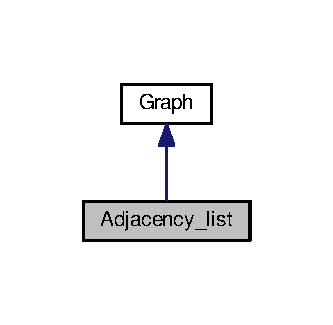
\includegraphics[width=160pt]{classAdjacency__list__inherit__graph}
\end{center}
\end{figure}


Collaboration diagram for Adjacency\-\_\-list\-:
\nopagebreak
\begin{figure}[H]
\begin{center}
\leavevmode
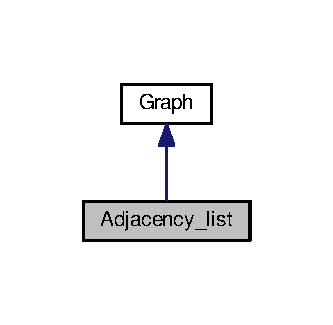
\includegraphics[width=160pt]{classAdjacency__list__coll__graph}
\end{center}
\end{figure}
\subsection*{Public Member Functions}
\begin{DoxyCompactItemize}
\item 
\hyperlink{classAdjacency__list_a7d5d3a9d4e555a56303fa9facc54f0ba}{Adjacency\-\_\-list} (str \hyperlink{classAdjacency__list_ab2eea0405522e8b9917d84ef44e70f66}{name})
\item 
\hyperlink{classAdjacency__list_a2a98e4275df4dc38fbfcdf84ec5ced7d}{Adjacency\-\_\-list} (str \hyperlink{classAdjacency__list_ab2eea0405522e8b9917d84ef44e70f66}{name}, std\-::shared\-\_\-ptr$<$ \hyperlink{structNode}{Node} $>$ \hyperlink{classAdjacency__list_a129aec8db0fc3b6109de60f765c41ac4}{start})
\item 
virtual \hyperlink{classAdjacency__list_a1eeb2fe43e777799b553b29135bcafd0}{$\sim$\-Adjacency\-\_\-list} ()
\item 
virtual void \hyperlink{classAdjacency__list_adbc9e5768336f17f7442638e5284f2a7}{add\-Node} (std\-::shared\-\_\-ptr$<$ \hyperlink{structNode}{Node} $>$ node)
\item 
virtual void \hyperlink{classAdjacency__list_a43a6325bc1e122a2675c39ea826f5f2a}{add\-Edge} (std\-::shared\-\_\-ptr$<$ \hyperlink{structNode}{Node} $>$ source, std\-::shared\-\_\-ptr$<$ \hyperlink{structNode}{Node} $>$ dist, bool path)
\item 
virtual N\-O\-D\-E\-S\-::iterator \hyperlink{classAdjacency__list_aca86880551fe5df685606de3a8ea0710}{begin} ()
\item 
virtual std\-::shared\-\_\-ptr$<$ \hyperlink{structNode}{Node} $>$ \hyperlink{classAdjacency__list_a129aec8db0fc3b6109de60f765c41ac4}{start} ()
\item 
virtual std\-::size\-\_\-t \hyperlink{classAdjacency__list_ac67e271d3a734fc596d678490101b509}{node\-Count} () const 
\item 
virtual std\-::shared\-\_\-ptr$<$ \hyperlink{structNode}{Node} $>$ \hyperlink{classAdjacency__list_aa15c2f8c06d2d3eee4e2f04002b728ab}{find} (int id) const 
\item 
virtual std\-::string \hyperlink{classAdjacency__list_ab2eea0405522e8b9917d84ef44e70f66}{name} () const 
\end{DoxyCompactItemize}


\subsection{Detailed Description}
Represents the implementation of the A\-S\-G interface as adjacency list. See documentation \hyperlink{classGraph}{Graph}.

\begin{DoxyAuthor}{Author}
Christopher Zell \href{mailto:Zelldon91@googlemail.com}{\tt Zelldon91@googlemail.\-com} 
\end{DoxyAuthor}


\subsection{Constructor \& Destructor Documentation}
\hypertarget{classAdjacency__list_a7d5d3a9d4e555a56303fa9facc54f0ba}{\index{Adjacency\-\_\-list@{Adjacency\-\_\-list}!Adjacency\-\_\-list@{Adjacency\-\_\-list}}
\index{Adjacency\-\_\-list@{Adjacency\-\_\-list}!Adjacency_list@{Adjacency\-\_\-list}}
\subsubsection[{Adjacency\-\_\-list}]{\setlength{\rightskip}{0pt plus 5cm}Adjacency\-\_\-list\-::\-Adjacency\-\_\-list (
\begin{DoxyParamCaption}
\item[{Adjacency\-\_\-list\-::str}]{name}
\end{DoxyParamCaption}
)}}\label{classAdjacency__list_a7d5d3a9d4e555a56303fa9facc54f0ba}
The ctor of the adjacency list, which gets the name of the Rail function. 
\begin{DoxyParams}{Parameters}
{\em name} & the name of the Rail function (A\-S\-G) \\
\hline
\end{DoxyParams}
\hypertarget{classAdjacency__list_a2a98e4275df4dc38fbfcdf84ec5ced7d}{\index{Adjacency\-\_\-list@{Adjacency\-\_\-list}!Adjacency\-\_\-list@{Adjacency\-\_\-list}}
\index{Adjacency\-\_\-list@{Adjacency\-\_\-list}!Adjacency_list@{Adjacency\-\_\-list}}
\subsubsection[{Adjacency\-\_\-list}]{\setlength{\rightskip}{0pt plus 5cm}Adjacency\-\_\-list\-::\-Adjacency\-\_\-list (
\begin{DoxyParamCaption}
\item[{Adjacency\-\_\-list\-::str}]{name, }
\item[{std\-::shared\-\_\-ptr$<$ {\bf Node} $>$}]{start}
\end{DoxyParamCaption}
)}}\label{classAdjacency__list_a2a98e4275df4dc38fbfcdf84ec5ced7d}
The ctor of the adjacency list, which gets the name of the Rail function and the first node. 
\begin{DoxyParams}{Parameters}
{\em name} & the name of the Rail function (A\-S\-G) \\
\hline
{\em start} & the start node of the Rail function \\
\hline
\end{DoxyParams}
\hypertarget{classAdjacency__list_a1eeb2fe43e777799b553b29135bcafd0}{\index{Adjacency\-\_\-list@{Adjacency\-\_\-list}!$\sim$\-Adjacency\-\_\-list@{$\sim$\-Adjacency\-\_\-list}}
\index{$\sim$\-Adjacency\-\_\-list@{$\sim$\-Adjacency\-\_\-list}!Adjacency_list@{Adjacency\-\_\-list}}
\subsubsection[{$\sim$\-Adjacency\-\_\-list}]{\setlength{\rightskip}{0pt plus 5cm}Adjacency\-\_\-list\-::$\sim$\-Adjacency\-\_\-list (
\begin{DoxyParamCaption}
{}
\end{DoxyParamCaption}
)\hspace{0.3cm}{\ttfamily [virtual]}}}\label{classAdjacency__list_a1eeb2fe43e777799b553b29135bcafd0}
The destructor of the adjacency list. Cleans up the nodes vector and resets the shared\-\_\-ptr's. 

\subsection{Member Function Documentation}
\hypertarget{classAdjacency__list_a43a6325bc1e122a2675c39ea826f5f2a}{\index{Adjacency\-\_\-list@{Adjacency\-\_\-list}!add\-Edge@{add\-Edge}}
\index{add\-Edge@{add\-Edge}!Adjacency_list@{Adjacency\-\_\-list}}
\subsubsection[{add\-Edge}]{\setlength{\rightskip}{0pt plus 5cm}void Adjacency\-\_\-list\-::add\-Edge (
\begin{DoxyParamCaption}
\item[{std\-::shared\-\_\-ptr$<$ {\bf Node} $>$}]{source, }
\item[{std\-::shared\-\_\-ptr$<$ {\bf Node} $>$}]{dist, }
\item[{bool}]{path}
\end{DoxyParamCaption}
)\hspace{0.3cm}{\ttfamily [virtual]}}}\label{classAdjacency__list_a43a6325bc1e122a2675c39ea826f5f2a}
Replaces the successor of a certain node. If the path is true the successor1 of the source will be replaced, successor2 if the path is false.


\begin{DoxyParams}{Parameters}
{\em source} & the node which gets a new succesor \\
\hline
{\em dist} & the new successor of the source \\
\hline
{\em path} & specifies whether the successor1 or 2 are been replaced \\
\hline
\end{DoxyParams}


Implements \hyperlink{classGraph_a9e45aafa60a807245e24565baea74a39}{Graph}.

\hypertarget{classAdjacency__list_adbc9e5768336f17f7442638e5284f2a7}{\index{Adjacency\-\_\-list@{Adjacency\-\_\-list}!add\-Node@{add\-Node}}
\index{add\-Node@{add\-Node}!Adjacency_list@{Adjacency\-\_\-list}}
\subsubsection[{add\-Node}]{\setlength{\rightskip}{0pt plus 5cm}void Adjacency\-\_\-list\-::add\-Node (
\begin{DoxyParamCaption}
\item[{std\-::shared\-\_\-ptr$<$ {\bf Node} $>$}]{node}
\end{DoxyParamCaption}
)\hspace{0.3cm}{\ttfamily [virtual]}}}\label{classAdjacency__list_adbc9e5768336f17f7442638e5284f2a7}




The implementation only adds the node if the node not already exists in the list. If the node exists, the node will be replaced by the new one. \par
 Inherited D\-O\-C\-: \par
 Adds a node (command) to the corresponding A\-S\-G.


\begin{DoxyParams}{Parameters}
{\em node} & the node which will be added \\
\hline
\end{DoxyParams}


Implements \hyperlink{classGraph_ae4ad7e42e8df191acd6563ca65ee779c}{Graph}.



Here is the call graph for this function\-:
\nopagebreak
\begin{figure}[H]
\begin{center}
\leavevmode
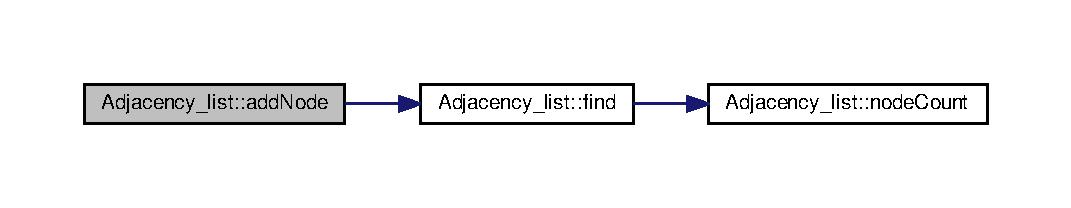
\includegraphics[width=350pt]{classAdjacency__list_adbc9e5768336f17f7442638e5284f2a7_cgraph}
\end{center}
\end{figure}


\hypertarget{classAdjacency__list_aca86880551fe5df685606de3a8ea0710}{\index{Adjacency\-\_\-list@{Adjacency\-\_\-list}!begin@{begin}}
\index{begin@{begin}!Adjacency_list@{Adjacency\-\_\-list}}
\subsubsection[{begin}]{\setlength{\rightskip}{0pt plus 5cm}Adjacency\-\_\-list\-::\-N\-O\-D\-E\-S\-::iterator Adjacency\-\_\-list\-::begin (
\begin{DoxyParamCaption}
{}
\end{DoxyParamCaption}
)\hspace{0.3cm}{\ttfamily [virtual]}}}\label{classAdjacency__list_aca86880551fe5df685606de3a8ea0710}
Returns the begin iterator of the nodes vector. \begin{DoxyReturn}{Returns}
the begin iterator of the nodes vector 
\end{DoxyReturn}
\hypertarget{classAdjacency__list_aa15c2f8c06d2d3eee4e2f04002b728ab}{\index{Adjacency\-\_\-list@{Adjacency\-\_\-list}!find@{find}}
\index{find@{find}!Adjacency_list@{Adjacency\-\_\-list}}
\subsubsection[{find}]{\setlength{\rightskip}{0pt plus 5cm}std\-::shared\-\_\-ptr$<$ {\bf Node} $>$ Adjacency\-\_\-list\-::find (
\begin{DoxyParamCaption}
\item[{int}]{id}
\end{DoxyParamCaption}
) const\hspace{0.3cm}{\ttfamily [virtual]}}}\label{classAdjacency__list_aa15c2f8c06d2d3eee4e2f04002b728ab}
Finds for the given id the node in the A\-S\-G. 
\begin{DoxyParams}{Parameters}
{\em id} & the id of the node, which should be founded \\
\hline
\end{DoxyParams}
\begin{DoxyReturn}{Returns}
the node with the searched id 
\end{DoxyReturn}


Implements \hyperlink{classGraph_aa37e2e2fd8d7ae9a94d4e174980644c6}{Graph}.



Here is the call graph for this function\-:
\nopagebreak
\begin{figure}[H]
\begin{center}
\leavevmode
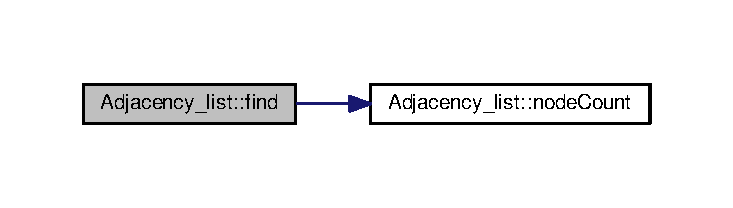
\includegraphics[width=350pt]{classAdjacency__list_aa15c2f8c06d2d3eee4e2f04002b728ab_cgraph}
\end{center}
\end{figure}


\hypertarget{classAdjacency__list_ab2eea0405522e8b9917d84ef44e70f66}{\index{Adjacency\-\_\-list@{Adjacency\-\_\-list}!name@{name}}
\index{name@{name}!Adjacency_list@{Adjacency\-\_\-list}}
\subsubsection[{name}]{\setlength{\rightskip}{0pt plus 5cm}std\-::string Adjacency\-\_\-list\-::name (
\begin{DoxyParamCaption}
{}
\end{DoxyParamCaption}
) const\hspace{0.3cm}{\ttfamily [virtual]}}}\label{classAdjacency__list_ab2eea0405522e8b9917d84ef44e70f66}
Returns the name of the A\-S\-G. The name of the graph is equal to the name of the Rail function. (Each function has his own graph) \begin{DoxyReturn}{Returns}
the name of the A\-S\-G 
\end{DoxyReturn}


Implements \hyperlink{classGraph_a0d1bc2d4425ddbef019b5d7589765c5a}{Graph}.

\hypertarget{classAdjacency__list_ac67e271d3a734fc596d678490101b509}{\index{Adjacency\-\_\-list@{Adjacency\-\_\-list}!node\-Count@{node\-Count}}
\index{node\-Count@{node\-Count}!Adjacency_list@{Adjacency\-\_\-list}}
\subsubsection[{node\-Count}]{\setlength{\rightskip}{0pt plus 5cm}std\-::size\-\_\-t Adjacency\-\_\-list\-::node\-Count (
\begin{DoxyParamCaption}
{}
\end{DoxyParamCaption}
) const\hspace{0.3cm}{\ttfamily [virtual]}}}\label{classAdjacency__list_ac67e271d3a734fc596d678490101b509}
Returns the current size of the graph (node count). \begin{DoxyReturn}{Returns}
the size of the A\-S\-G 
\end{DoxyReturn}


Implements \hyperlink{classGraph_afed2883e765871cc439b08d9aeba028b}{Graph}.

\hypertarget{classAdjacency__list_a129aec8db0fc3b6109de60f765c41ac4}{\index{Adjacency\-\_\-list@{Adjacency\-\_\-list}!start@{start}}
\index{start@{start}!Adjacency_list@{Adjacency\-\_\-list}}
\subsubsection[{start}]{\setlength{\rightskip}{0pt plus 5cm}std\-::shared\-\_\-ptr$<$ {\bf Node} $>$ Adjacency\-\_\-list\-::start (
\begin{DoxyParamCaption}
{}
\end{DoxyParamCaption}
)\hspace{0.3cm}{\ttfamily [virtual]}}}\label{classAdjacency__list_a129aec8db0fc3b6109de60f765c41ac4}
Returns the start node of the A\-S\-G, respectively of the Rail function. \begin{DoxyReturn}{Returns}
the start node 
\end{DoxyReturn}


Implements \hyperlink{classGraph_a7b0c57d46c652fb12e4ca65a816f7a36}{Graph}.



Here is the call graph for this function\-:
\nopagebreak
\begin{figure}[H]
\begin{center}
\leavevmode
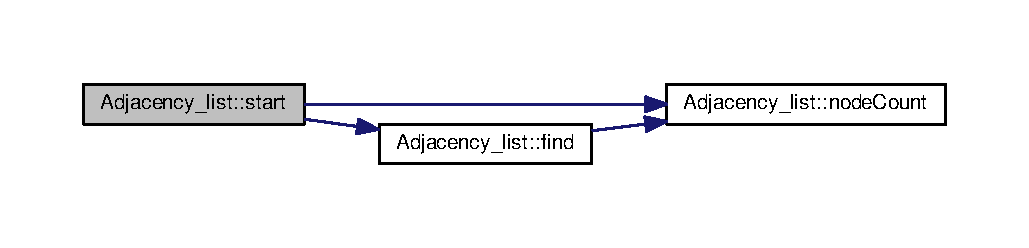
\includegraphics[width=350pt]{classAdjacency__list_a129aec8db0fc3b6109de60f765c41ac4_cgraph}
\end{center}
\end{figure}




The documentation for this class was generated from the following files\-:\begin{DoxyCompactItemize}
\item 
frontend/\hyperlink{adjacency__list_8h}{adjacency\-\_\-list.\-h}\item 
frontend/\hyperlink{adjacency__list_8cpp}{adjacency\-\_\-list.\-cpp}\end{DoxyCompactItemize}

\hypertarget{structallowedChars}{\section{allowed\-Chars Struct Reference}
\label{structallowedChars}\index{allowed\-Chars@{allowed\-Chars}}
}


{\ttfamily \#include $<$Parser.\-h$>$}

\subsection*{Public Attributes}
\begin{DoxyCompactItemize}
\item 
list$<$ char $>$ \hyperlink{structallowedChars_aa455ccda98e8c550c1b7cf7bc8dcabcd}{left}
\item 
list$<$ char $>$ \hyperlink{structallowedChars_a7d7caec9cd32a1a362e845a38ef1561c}{straight}
\item 
list$<$ char $>$ \hyperlink{structallowedChars_a2aa7cf42bc94729fc3f5d3004d60d662}{right}
\end{DoxyCompactItemize}


\subsection{Member Data Documentation}
\hypertarget{structallowedChars_aa455ccda98e8c550c1b7cf7bc8dcabcd}{\index{allowed\-Chars@{allowed\-Chars}!left@{left}}
\index{left@{left}!allowedChars@{allowed\-Chars}}
\subsubsection[{left}]{\setlength{\rightskip}{0pt plus 5cm}list$<$char$>$ allowed\-Chars\-::left}}\label{structallowedChars_aa455ccda98e8c550c1b7cf7bc8dcabcd}
\hypertarget{structallowedChars_a2aa7cf42bc94729fc3f5d3004d60d662}{\index{allowed\-Chars@{allowed\-Chars}!right@{right}}
\index{right@{right}!allowedChars@{allowed\-Chars}}
\subsubsection[{right}]{\setlength{\rightskip}{0pt plus 5cm}list$<$char$>$ allowed\-Chars\-::right}}\label{structallowedChars_a2aa7cf42bc94729fc3f5d3004d60d662}
\hypertarget{structallowedChars_a7d7caec9cd32a1a362e845a38ef1561c}{\index{allowed\-Chars@{allowed\-Chars}!straight@{straight}}
\index{straight@{straight}!allowedChars@{allowed\-Chars}}
\subsubsection[{straight}]{\setlength{\rightskip}{0pt plus 5cm}list$<$char$>$ allowed\-Chars\-::straight}}\label{structallowedChars_a7d7caec9cd32a1a362e845a38ef1561c}


The documentation for this struct was generated from the following file\-:\begin{DoxyCompactItemize}
\item 
frontend/\hyperlink{Parser_8h}{Parser.\-h}\end{DoxyCompactItemize}

\hypertarget{classBackend}{\section{Backend Class Reference}
\label{classBackend}\index{Backend@{Backend}}
}


{\ttfamily \#include $<$backend.\-h$>$}

\subsection*{Public Types}
\begin{DoxyCompactItemize}
\item 
enum \hyperlink{classBackend_a0e8eebed86bd15218f21b068f6c229f2}{Status} \{ \hyperlink{classBackend_a0e8eebed86bd15218f21b068f6c229f2a85c3bbdd79e0c08753992d41f8a7d25c}{S\-U\-C\-C\-E\-S\-S}
 \}
\end{DoxyCompactItemize}
\subsection*{Static Public Member Functions}
\begin{DoxyCompactItemize}
\item 
static \hyperlink{classBackend_a0e8eebed86bd15218f21b068f6c229f2}{Backend\-::\-Status} \hyperlink{classBackend_aa3ad5ea4b71dac952445fbe3762b4d88}{Generate} (const std\-::string \&filename, std\-::ostream \&code\-Out)
\item 
static \hyperlink{classBackend_a0e8eebed86bd15218f21b068f6c229f2}{Backend\-::\-Status} \hyperlink{classBackend_a33fce3d0ea3e4b7038ffb0dbf5503a27}{Generate} (\hyperlink{classGraphs}{Graphs} \&graphs, std\-::ostream \&code\-Out)
\item 
static std\-::string \hyperlink{classBackend_a72370277408a5586b5923bc56433b815}{Error\-Message} (\hyperlink{classBackend_a0e8eebed86bd15218f21b068f6c229f2}{Backend\-::\-Status} status)
\end{DoxyCompactItemize}


\subsection{Detailed Description}
Die Klasse stellt statische Methoden für das Übersetzen des Graphen in Target-\/\-Code zur Verfügung. 

\subsection{Member Enumeration Documentation}
\hypertarget{classBackend_a0e8eebed86bd15218f21b068f6c229f2}{\index{Backend@{Backend}!Status@{Status}}
\index{Status@{Status}!Backend@{Backend}}
\subsubsection[{Status}]{\setlength{\rightskip}{0pt plus 5cm}enum {\bf Backend\-::\-Status}}}\label{classBackend_a0e8eebed86bd15218f21b068f6c229f2}
Die möglichen 'Exit Codes' des Backends. \begin{Desc}
\item[Enumerator]\par
\begin{description}
\index{S\-U\-C\-C\-E\-S\-S@{S\-U\-C\-C\-E\-S\-S}!Backend@{Backend}}\index{Backend@{Backend}!S\-U\-C\-C\-E\-S\-S@{S\-U\-C\-C\-E\-S\-S}}\item[{\em 
\hypertarget{classBackend_a0e8eebed86bd15218f21b068f6c229f2a85c3bbdd79e0c08753992d41f8a7d25c}{S\-U\-C\-C\-E\-S\-S}\label{classBackend_a0e8eebed86bd15218f21b068f6c229f2a85c3bbdd79e0c08753992d41f8a7d25c}
}]Erfolgreiche Übersetzung. \end{description}
\end{Desc}


\subsection{Member Function Documentation}
\hypertarget{classBackend_a72370277408a5586b5923bc56433b815}{\index{Backend@{Backend}!Error\-Message@{Error\-Message}}
\index{Error\-Message@{Error\-Message}!Backend@{Backend}}
\subsubsection[{Error\-Message}]{\setlength{\rightskip}{0pt plus 5cm}std\-::string Backend\-::\-Error\-Message (
\begin{DoxyParamCaption}
\item[{{\bf Backend\-::\-Status}}]{status}
\end{DoxyParamCaption}
)\hspace{0.3cm}{\ttfamily [static]}}}\label{classBackend_a72370277408a5586b5923bc56433b815}
Gibt eine beschreibende Fehlernachricht zu einem \hyperlink{classBackend_a0e8eebed86bd15218f21b068f6c229f2}{Backend\-::\-Status} zurück. Ist der status Backend\-::\-Status\-::\-S\-U\-C\-C\-E\-S\-S, wird ein leerer String zurückgegeben. Typische Nutzung dieser Methode\-: if (status != Backend\-::\-Status\-::\-S\-U\-C\-C\-E\-S\-S) \{ std\-::cerr $<$$<$ Backend\-::\-Error\-Message(status) $<$$<$ std\-::endl; \} \hypertarget{classBackend_aa3ad5ea4b71dac952445fbe3762b4d88}{\index{Backend@{Backend}!Generate@{Generate}}
\index{Generate@{Generate}!Backend@{Backend}}
\subsubsection[{Generate}]{\setlength{\rightskip}{0pt plus 5cm}{\bf Backend\-::\-Status} Backend\-::\-Generate (
\begin{DoxyParamCaption}
\item[{const std\-::string \&}]{filename, }
\item[{std\-::ostream \&}]{code\-Out}
\end{DoxyParamCaption}
)\hspace{0.3cm}{\ttfamily [static]}}}\label{classBackend_aa3ad5ea4b71dac952445fbe3762b4d88}
Übersetzt den serialisierten Graphen aus graph\-In (Dateiname) in Target-\/\-Code, der auf code\-Out geschrieben wird. Gibt je nach Ergebnis einen \hyperlink{classBackend_a0e8eebed86bd15218f21b068f6c229f2}{Backend\-::\-Status} zurück. 

Here is the call graph for this function\-:
\nopagebreak
\begin{figure}[H]
\begin{center}
\leavevmode
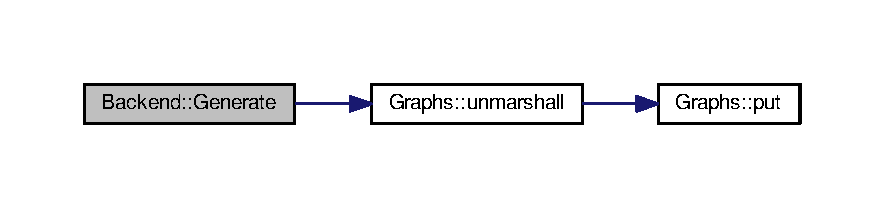
\includegraphics[width=350pt]{classBackend_aa3ad5ea4b71dac952445fbe3762b4d88_cgraph}
\end{center}
\end{figure}


\hypertarget{classBackend_a33fce3d0ea3e4b7038ffb0dbf5503a27}{\index{Backend@{Backend}!Generate@{Generate}}
\index{Generate@{Generate}!Backend@{Backend}}
\subsubsection[{Generate}]{\setlength{\rightskip}{0pt plus 5cm}{\bf Backend\-::\-Status} Backend\-::\-Generate (
\begin{DoxyParamCaption}
\item[{{\bf Graphs} \&}]{graphs, }
\item[{std\-::ostream \&}]{code\-Out}
\end{DoxyParamCaption}
)\hspace{0.3cm}{\ttfamily [static]}}}\label{classBackend_a33fce3d0ea3e4b7038ffb0dbf5503a27}
Übersetzt den Graphen aus graph in Target-\/\-Code, der auf code\-Out geschrieben wird. Gibt je nach Ergebnis einen \hyperlink{classBackend_a0e8eebed86bd15218f21b068f6c229f2}{Backend\-::\-Status} zurück. 

Here is the call graph for this function\-:
\nopagebreak
\begin{figure}[H]
\begin{center}
\leavevmode
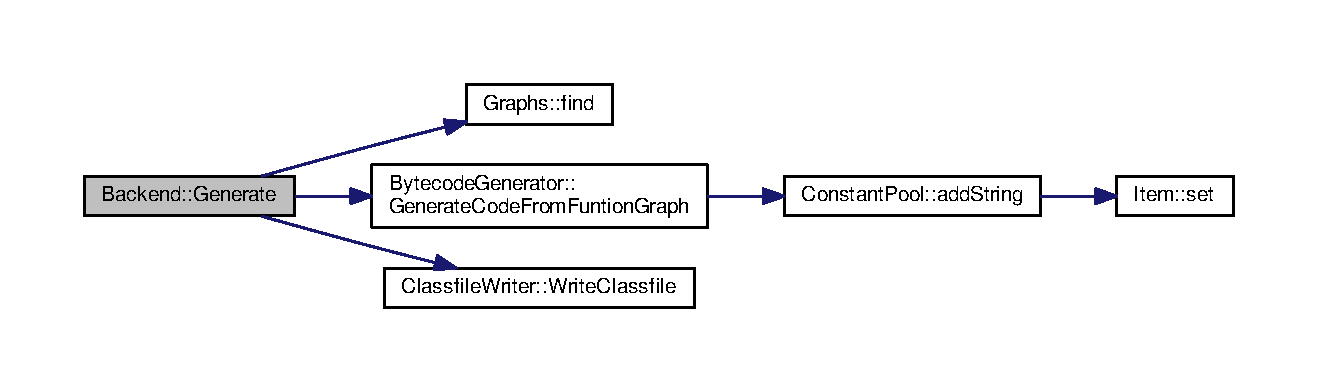
\includegraphics[width=350pt]{classBackend_a33fce3d0ea3e4b7038ffb0dbf5503a27_cgraph}
\end{center}
\end{figure}




The documentation for this class was generated from the following files\-:\begin{DoxyCompactItemize}
\item 
backend/\hyperlink{backend_8h}{backend.\-h}\item 
backend/\hyperlink{backend_8cc}{backend.\-cc}\end{DoxyCompactItemize}

\hypertarget{structBoardContainer}{\section{Board\-Container Struct Reference}
\label{structBoardContainer}\index{Board\-Container@{Board\-Container}}
}


{\ttfamily \#include $<$Parser.\-h$>$}

\subsection*{Public Attributes}
\begin{DoxyCompactItemize}
\item 
char($\ast$ \hyperlink{structBoardContainer_ac48c8d00315c6ba23b92c49a555bc340}{board} )\mbox{[}1024\mbox{]}
\item 
int \hyperlink{structBoardContainer_a8c8f5a08f1a20aa38da2e69d0fdef48b}{xlen}
\item 
int \hyperlink{structBoardContainer_ac438366505cda656d08223d5378caa8f}{ylen}
\end{DoxyCompactItemize}


\subsection{Member Data Documentation}
\hypertarget{structBoardContainer_ac48c8d00315c6ba23b92c49a555bc340}{\index{Board\-Container@{Board\-Container}!board@{board}}
\index{board@{board}!BoardContainer@{Board\-Container}}
\subsubsection[{board}]{\setlength{\rightskip}{0pt plus 5cm}char($\ast$ Board\-Container\-::board)\mbox{[}1024\mbox{]}}}\label{structBoardContainer_ac48c8d00315c6ba23b92c49a555bc340}
\hypertarget{structBoardContainer_a8c8f5a08f1a20aa38da2e69d0fdef48b}{\index{Board\-Container@{Board\-Container}!xlen@{xlen}}
\index{xlen@{xlen}!BoardContainer@{Board\-Container}}
\subsubsection[{xlen}]{\setlength{\rightskip}{0pt plus 5cm}int Board\-Container\-::xlen}}\label{structBoardContainer_a8c8f5a08f1a20aa38da2e69d0fdef48b}
\hypertarget{structBoardContainer_ac438366505cda656d08223d5378caa8f}{\index{Board\-Container@{Board\-Container}!ylen@{ylen}}
\index{ylen@{ylen}!BoardContainer@{Board\-Container}}
\subsubsection[{ylen}]{\setlength{\rightskip}{0pt plus 5cm}int Board\-Container\-::ylen}}\label{structBoardContainer_ac438366505cda656d08223d5378caa8f}


The documentation for this struct was generated from the following file\-:\begin{DoxyCompactItemize}
\item 
frontend/\hyperlink{Parser_8h}{Parser.\-h}\end{DoxyCompactItemize}

\hypertarget{classBytecodeGenerator}{\section{Bytecode\-Generator Class Reference}
\label{classBytecodeGenerator}\index{Bytecode\-Generator@{Bytecode\-Generator}}
}


{\ttfamily \#include $<$bytecode\-\_\-generator.\-h$>$}

\subsection*{Static Public Member Functions}
\begin{DoxyCompactItemize}
\item 
static std\-::vector$<$ char $>$ \hyperlink{classBytecodeGenerator_a3e352fea6159f2c4bb48ec9b3d532672}{Generate\-Code\-From\-Funtion\-Graph} (\hyperlink{classGraphs_a58b4b65d81870fc3b2936c068b644a4d}{Graphs\-::\-Graph\-\_\-ptr} graph, \hyperlink{classConstantPool}{Constant\-Pool} \&constant\-Pool)
\end{DoxyCompactItemize}


\subsection{Member Function Documentation}
\hypertarget{classBytecodeGenerator_a3e352fea6159f2c4bb48ec9b3d532672}{\index{Bytecode\-Generator@{Bytecode\-Generator}!Generate\-Code\-From\-Funtion\-Graph@{Generate\-Code\-From\-Funtion\-Graph}}
\index{Generate\-Code\-From\-Funtion\-Graph@{Generate\-Code\-From\-Funtion\-Graph}!BytecodeGenerator@{Bytecode\-Generator}}
\subsubsection[{Generate\-Code\-From\-Funtion\-Graph}]{\setlength{\rightskip}{0pt plus 5cm}std\-::vector$<$ char $>$ Bytecode\-Generator\-::\-Generate\-Code\-From\-Funtion\-Graph (
\begin{DoxyParamCaption}
\item[{{\bf Graphs\-::\-Graph\-\_\-ptr}}]{graph, }
\item[{{\bf Constant\-Pool} \&}]{constant\-Pool}
\end{DoxyParamCaption}
)\hspace{0.3cm}{\ttfamily [static]}}}\label{classBytecodeGenerator_a3e352fea6159f2c4bb48ec9b3d532672}


Here is the call graph for this function\-:
\nopagebreak
\begin{figure}[H]
\begin{center}
\leavevmode
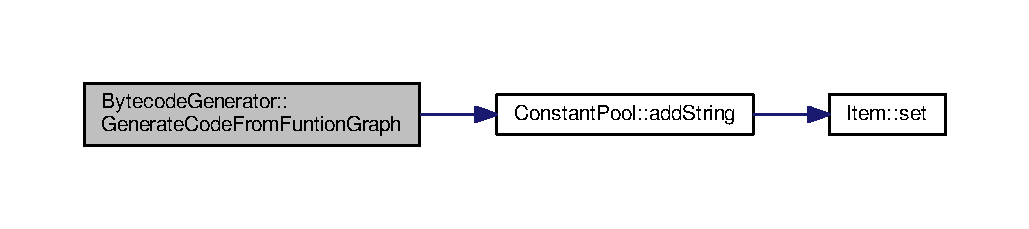
\includegraphics[width=350pt]{classBytecodeGenerator_a3e352fea6159f2c4bb48ec9b3d532672_cgraph}
\end{center}
\end{figure}




The documentation for this class was generated from the following files\-:\begin{DoxyCompactItemize}
\item 
backend/codegen/\hyperlink{bytecode__generator_8h}{bytecode\-\_\-generator.\-h}\item 
backend/codegen/\hyperlink{bytecode__generator_8cpp}{bytecode\-\_\-generator.\-cpp}\end{DoxyCompactItemize}

\hypertarget{classClassfileWriter}{\section{Classfile\-Writer Class Reference}
\label{classClassfileWriter}\index{Classfile\-Writer@{Classfile\-Writer}}
}


{\ttfamily \#include $<$classfile\-\_\-writer.\-h$>$}

\subsection*{Public Types}
\begin{DoxyCompactItemize}
\item 
enum \hyperlink{classClassfileWriter_ad1f8ad574818eb3e851f3c99ba6cc8f2}{Classfile\-Version} \{ \hyperlink{classClassfileWriter_ad1f8ad574818eb3e851f3c99ba6cc8f2af3b45f7e6d21c22615772ad808043633}{J\-A\-V\-A\-\_\-7}
 \}
\end{DoxyCompactItemize}
\subsection*{Public Member Functions}
\begin{DoxyCompactItemize}
\item 
\hyperlink{classClassfileWriter_afbc090a3af8847ec859093e33ddd28e8}{Classfile\-Writer} (\hyperlink{classClassfileWriter_ad1f8ad574818eb3e851f3c99ba6cc8f2}{Classfile\-Version} version, const \hyperlink{classConstantPool}{Constant\-Pool} \&constant\-Pool, const std\-::map$<$ std\-::string, std\-::vector$<$ char $>$ \& $>$ code\-Functions, std\-::ostream \&out)
\item 
virtual \hyperlink{classClassfileWriter_ab72a8243f08eb03cbfdd517121d2f1d2}{$\sim$\-Classfile\-Writer} ()
\item 
void \hyperlink{classClassfileWriter_a578ae6492320adc125ec2aaf13ad65c6}{Write\-Classfile} ()
\end{DoxyCompactItemize}


\subsection{Detailed Description}
Klasse zum Schreiben einer einfachen .class-\/\-Datei (Nur Methoden, keine Fields, keine Vererbung) auf einen Stream. 

\subsection{Member Enumeration Documentation}
\hypertarget{classClassfileWriter_ad1f8ad574818eb3e851f3c99ba6cc8f2}{\index{Classfile\-Writer@{Classfile\-Writer}!Classfile\-Version@{Classfile\-Version}}
\index{Classfile\-Version@{Classfile\-Version}!ClassfileWriter@{Classfile\-Writer}}
\subsubsection[{Classfile\-Version}]{\setlength{\rightskip}{0pt plus 5cm}enum {\bf Classfile\-Writer\-::\-Classfile\-Version}}}\label{classClassfileWriter_ad1f8ad574818eb3e851f3c99ba6cc8f2}
Die Versionsnummer der zu schreibenden .class-\/\-Datei. \begin{Desc}
\item[Enumerator]\par
\begin{description}
\index{J\-A\-V\-A\-\_\-7@{J\-A\-V\-A\-\_\-7}!Classfile\-Writer@{Classfile\-Writer}}\index{Classfile\-Writer@{Classfile\-Writer}!J\-A\-V\-A\-\_\-7@{J\-A\-V\-A\-\_\-7}}\item[{\em 
\hypertarget{classClassfileWriter_ad1f8ad574818eb3e851f3c99ba6cc8f2af3b45f7e6d21c22615772ad808043633}{J\-A\-V\-A\-\_\-7}\label{classClassfileWriter_ad1f8ad574818eb3e851f3c99ba6cc8f2af3b45f7e6d21c22615772ad808043633}
}]\end{description}
\end{Desc}


\subsection{Constructor \& Destructor Documentation}
\hypertarget{classClassfileWriter_afbc090a3af8847ec859093e33ddd28e8}{\index{Classfile\-Writer@{Classfile\-Writer}!Classfile\-Writer@{Classfile\-Writer}}
\index{Classfile\-Writer@{Classfile\-Writer}!ClassfileWriter@{Classfile\-Writer}}
\subsubsection[{Classfile\-Writer}]{\setlength{\rightskip}{0pt plus 5cm}Classfile\-Writer\-::\-Classfile\-Writer (
\begin{DoxyParamCaption}
\item[{{\bf Classfile\-Version}}]{version, }
\item[{const {\bf Constant\-Pool} \&}]{constant\-Pool, }
\item[{const std\-::map$<$ std\-::string, std\-::vector$<$ char $>$ \& $>$}]{code\-Functions, }
\item[{std\-::ostream \&}]{out}
\end{DoxyParamCaption}
)}}\label{classClassfileWriter_afbc090a3af8847ec859093e33ddd28e8}
Erstellt einen neuen Writer zum Schreiben einer .class-\/\-Datei der Version 'version' mit dem \hyperlink{classConstantPool}{Constant\-Pool} 'constant\-Pool' auf den Stream 'out'. Der Bytecode wird in der map 'code\-Functions' gehalten, Map Funktionsname -\/$>$ Bytecode. \hypertarget{classClassfileWriter_ab72a8243f08eb03cbfdd517121d2f1d2}{\index{Classfile\-Writer@{Classfile\-Writer}!$\sim$\-Classfile\-Writer@{$\sim$\-Classfile\-Writer}}
\index{$\sim$\-Classfile\-Writer@{$\sim$\-Classfile\-Writer}!ClassfileWriter@{Classfile\-Writer}}
\subsubsection[{$\sim$\-Classfile\-Writer}]{\setlength{\rightskip}{0pt plus 5cm}Classfile\-Writer\-::$\sim$\-Classfile\-Writer (
\begin{DoxyParamCaption}
{}
\end{DoxyParamCaption}
)\hspace{0.3cm}{\ttfamily [virtual]}}}\label{classClassfileWriter_ab72a8243f08eb03cbfdd517121d2f1d2}


\subsection{Member Function Documentation}
\hypertarget{classClassfileWriter_a578ae6492320adc125ec2aaf13ad65c6}{\index{Classfile\-Writer@{Classfile\-Writer}!Write\-Classfile@{Write\-Classfile}}
\index{Write\-Classfile@{Write\-Classfile}!ClassfileWriter@{Classfile\-Writer}}
\subsubsection[{Write\-Classfile}]{\setlength{\rightskip}{0pt plus 5cm}void Classfile\-Writer\-::\-Write\-Classfile (
\begin{DoxyParamCaption}
{}
\end{DoxyParamCaption}
)}}\label{classClassfileWriter_a578ae6492320adc125ec2aaf13ad65c6}
Schreibt die durch diesen Writer festgelegte .class-\/\-Datei auf den Ausgabestream. 

The documentation for this class was generated from the following files\-:\begin{DoxyCompactItemize}
\item 
backend/classfile/\hyperlink{classfile__writer_8h}{classfile\-\_\-writer.\-h}\item 
backend/classfile/\hyperlink{classfile__writer_8cc}{classfile\-\_\-writer.\-cc}\end{DoxyCompactItemize}

\hypertarget{structCommand}{\section{Command Struct Reference}
\label{structCommand}\index{Command@{Command}}
}


{\ttfamily \#include $<$ast.\-h$>$}

\subsection*{Public Types}
\begin{DoxyCompactItemize}
\item 
enum \hyperlink{structCommand_a4ca33b8d40e12deca5e7bb4190426ee1}{Type} \{ \\*
\hyperlink{structCommand_a4ca33b8d40e12deca5e7bb4190426ee1aa9601dbf610b9d23ee4b8b7bd378175e}{P\-U\-S\-H\-\_\-\-C\-O\-N\-S\-T} = 0, 
\hyperlink{structCommand_a4ca33b8d40e12deca5e7bb4190426ee1ab8db68a1487bc3f5dc3a9289e6a3b761}{C\-A\-L\-L} = 1, 
\hyperlink{structCommand_a4ca33b8d40e12deca5e7bb4190426ee1a6fbf52940c97a769906201ea768361c6}{O\-U\-T\-P\-U\-T} = 111, 
\hyperlink{structCommand_a4ca33b8d40e12deca5e7bb4190426ee1a1189491a065b6e6ca344cad213b618ff}{A\-D\-D} = 97, 
\\*
\hyperlink{structCommand_a4ca33b8d40e12deca5e7bb4190426ee1a7e3944da56a06f7078ade3e53cfbb215}{S\-U\-B} = 115, 
\hyperlink{structCommand_a4ca33b8d40e12deca5e7bb4190426ee1a7b47a91ef35876e3a36f215ca67cc52a}{M\-U\-L\-T} = 109, 
\hyperlink{structCommand_a4ca33b8d40e12deca5e7bb4190426ee1a4f9f14e8f597144f5581e4c11717f996}{D\-I\-V} = 100, 
\hyperlink{structCommand_a4ca33b8d40e12deca5e7bb4190426ee1aa5385a05c6b3340821284c63596512fb}{M\-O\-D} = 114, 
\\*
\hyperlink{structCommand_a4ca33b8d40e12deca5e7bb4190426ee1ae881b6fa7ec6fcd5f5e48de9a5e47357}{C\-U\-T} = 99, 
\hyperlink{structCommand_a4ca33b8d40e12deca5e7bb4190426ee1aba5756bd7d42e6770814802b30748cb4}{A\-P\-P\-E\-N\-D} = 112, 
\hyperlink{structCommand_a4ca33b8d40e12deca5e7bb4190426ee1a48428a4d51c5dde2f606aac5b8fc8c8e}{S\-I\-Z\-E} = 122, 
\hyperlink{structCommand_a4ca33b8d40e12deca5e7bb4190426ee1aba36ce21d1a872f0eb69fbb2ecccb872}{N\-I\-L} = 110, 
\\*
\hyperlink{structCommand_a4ca33b8d40e12deca5e7bb4190426ee1a230daeb879328f6570fc0137a8ba8b8a}{L\-I\-S\-T\-\_\-\-C\-O\-N\-S} = 58, 
\hyperlink{structCommand_a4ca33b8d40e12deca5e7bb4190426ee1a20bc54e7f190aca7865d4dc27f2b6489}{L\-I\-S\-T\-\_\-\-B\-R\-E\-A\-K\-U\-P} = 126, 
\hyperlink{structCommand_a4ca33b8d40e12deca5e7bb4190426ee1a9b0bf72679374cdefb0c3f0c1965faef}{F\-A\-L\-S\-E} = 102, 
\hyperlink{structCommand_a4ca33b8d40e12deca5e7bb4190426ee1a1e91eb5b37ab7cc6f9ff0e773e8a47a5}{G\-R\-E\-A\-T\-E\-R} = 103, 
\\*
\hyperlink{structCommand_a4ca33b8d40e12deca5e7bb4190426ee1ac7cb579e3efb508f2ce9162c7fc4f894}{E\-Q\-U\-A\-L} = 113, 
\hyperlink{structCommand_a4ca33b8d40e12deca5e7bb4190426ee1af4a87f4688672121e2c76e20f4360391}{T\-R\-U\-E} = 116, 
\hyperlink{structCommand_a4ca33b8d40e12deca5e7bb4190426ee1a6266090f9a24e8780fcc58bbd3f3e433}{R\-E\-F\-L\-E\-C\-T\-O\-R} = 64, 
\hyperlink{structCommand_a4ca33b8d40e12deca5e7bb4190426ee1a3972753fd8c0c1d6d908c9691e740f4f}{S\-T\-A\-R\-T} = 36, 
\\*
\hyperlink{structCommand_a4ca33b8d40e12deca5e7bb4190426ee1af28ab76d25c104e01b8325a337558c21}{F\-I\-N\-I\-S\-H} = 35, 
\hyperlink{structCommand_a4ca33b8d40e12deca5e7bb4190426ee1a7ac408d60d087c6290f1e5eb7c16ba87}{L\-A\-M\-B\-D\-A} = 38, 
\hyperlink{structCommand_a4ca33b8d40e12deca5e7bb4190426ee1a4bea7fb36a4d87ca49e9944b5ca09ee4}{B\-O\-O\-M} = 98, 
\hyperlink{structCommand_a4ca33b8d40e12deca5e7bb4190426ee1acde4d704509b525b7d867d393d478a7a}{E\-O\-F\-\_\-\-C\-H\-E\-C\-K} = 101, 
\\*
\hyperlink{structCommand_a4ca33b8d40e12deca5e7bb4190426ee1ac1fa13fd13ccf87b7a1ff32aa521625e}{I\-N\-P\-U\-T} = 105, 
\hyperlink{structCommand_a4ca33b8d40e12deca5e7bb4190426ee1a9335b6cbcc604c61c8c851fe53baac28}{U\-N\-D\-E\-R\-F\-L\-O\-W\-\_\-\-C\-H\-E\-C\-K} = 117, 
\hyperlink{structCommand_a4ca33b8d40e12deca5e7bb4190426ee1a042a811243865383719e6d6e889ee7e1}{T\-Y\-P\-E\-\_\-\-C\-H\-E\-C\-K} = 63
 \}
\end{DoxyCompactItemize}
\subsection*{Public Attributes}
\begin{DoxyCompactItemize}
\item 
\hyperlink{structCommand_a4ca33b8d40e12deca5e7bb4190426ee1}{Command\-::\-Type} \hyperlink{structCommand_a9b682ee6829f8aa99c936997b9107686}{type}
\item 
std\-::string \hyperlink{structCommand_a2764694100839fad40df1dfd7be7145a}{arg}
\end{DoxyCompactItemize}


\subsection{Detailed Description}
Represents an Rail command, consits of an enum \hyperlink{structCommand_a4ca33b8d40e12deca5e7bb4190426ee1}{Command\-::\-Type} and an argument. For each command type in Rail there exists a corresponding enum \hyperlink{structCommand_a4ca33b8d40e12deca5e7bb4190426ee1}{Command\-::\-Type}.

\begin{DoxyAuthor}{Author}
Christopher Zell \href{mailto:Zelldon91@googlemail.com}{\tt Zelldon91@googlemail.\-com}, Hanin Halawani 
\end{DoxyAuthor}


\subsection{Member Enumeration Documentation}
\hypertarget{structCommand_a4ca33b8d40e12deca5e7bb4190426ee1}{\index{Command@{Command}!Type@{Type}}
\index{Type@{Type}!Command@{Command}}
\subsubsection[{Type}]{\setlength{\rightskip}{0pt plus 5cm}enum {\bf Command\-::\-Type}}}\label{structCommand_a4ca33b8d40e12deca5e7bb4190426ee1}
Represents an command type of an Rail progamm. Each value corresponds to the ascii value of the corresponding Rail command. E.\-g. o -\/$>$ 111 or a -\/$>$ 97, thats makes the mapping much easier. \begin{Desc}
\item[Enumerator]\par
\begin{description}
\index{P\-U\-S\-H\-\_\-\-C\-O\-N\-S\-T@{P\-U\-S\-H\-\_\-\-C\-O\-N\-S\-T}!Command@{Command}}\index{Command@{Command}!P\-U\-S\-H\-\_\-\-C\-O\-N\-S\-T@{P\-U\-S\-H\-\_\-\-C\-O\-N\-S\-T}}\item[{\em 
\hypertarget{structCommand_a4ca33b8d40e12deca5e7bb4190426ee1aa9601dbf610b9d23ee4b8b7bd378175e}{P\-U\-S\-H\-\_\-\-C\-O\-N\-S\-T}\label{structCommand_a4ca33b8d40e12deca5e7bb4190426ee1aa9601dbf610b9d23ee4b8b7bd378175e}
}]0-\/9 or \mbox{[}...\mbox{]} \index{C\-A\-L\-L@{C\-A\-L\-L}!Command@{Command}}\index{Command@{Command}!C\-A\-L\-L@{C\-A\-L\-L}}\item[{\em 
\hypertarget{structCommand_a4ca33b8d40e12deca5e7bb4190426ee1ab8db68a1487bc3f5dc3a9289e6a3b761}{C\-A\-L\-L}\label{structCommand_a4ca33b8d40e12deca5e7bb4190426ee1ab8db68a1487bc3f5dc3a9289e6a3b761}
}]\{F\-U\-N\-C\} \index{O\-U\-T\-P\-U\-T@{O\-U\-T\-P\-U\-T}!Command@{Command}}\index{Command@{Command}!O\-U\-T\-P\-U\-T@{O\-U\-T\-P\-U\-T}}\item[{\em 
\hypertarget{structCommand_a4ca33b8d40e12deca5e7bb4190426ee1a6fbf52940c97a769906201ea768361c6}{O\-U\-T\-P\-U\-T}\label{structCommand_a4ca33b8d40e12deca5e7bb4190426ee1a6fbf52940c97a769906201ea768361c6}
}]o \index{A\-D\-D@{A\-D\-D}!Command@{Command}}\index{Command@{Command}!A\-D\-D@{A\-D\-D}}\item[{\em 
\hypertarget{structCommand_a4ca33b8d40e12deca5e7bb4190426ee1a1189491a065b6e6ca344cad213b618ff}{A\-D\-D}\label{structCommand_a4ca33b8d40e12deca5e7bb4190426ee1a1189491a065b6e6ca344cad213b618ff}
}]a \index{S\-U\-B@{S\-U\-B}!Command@{Command}}\index{Command@{Command}!S\-U\-B@{S\-U\-B}}\item[{\em 
\hypertarget{structCommand_a4ca33b8d40e12deca5e7bb4190426ee1a7e3944da56a06f7078ade3e53cfbb215}{S\-U\-B}\label{structCommand_a4ca33b8d40e12deca5e7bb4190426ee1a7e3944da56a06f7078ade3e53cfbb215}
}]s \index{M\-U\-L\-T@{M\-U\-L\-T}!Command@{Command}}\index{Command@{Command}!M\-U\-L\-T@{M\-U\-L\-T}}\item[{\em 
\hypertarget{structCommand_a4ca33b8d40e12deca5e7bb4190426ee1a7b47a91ef35876e3a36f215ca67cc52a}{M\-U\-L\-T}\label{structCommand_a4ca33b8d40e12deca5e7bb4190426ee1a7b47a91ef35876e3a36f215ca67cc52a}
}]m \index{D\-I\-V@{D\-I\-V}!Command@{Command}}\index{Command@{Command}!D\-I\-V@{D\-I\-V}}\item[{\em 
\hypertarget{structCommand_a4ca33b8d40e12deca5e7bb4190426ee1a4f9f14e8f597144f5581e4c11717f996}{D\-I\-V}\label{structCommand_a4ca33b8d40e12deca5e7bb4190426ee1a4f9f14e8f597144f5581e4c11717f996}
}]d \index{M\-O\-D@{M\-O\-D}!Command@{Command}}\index{Command@{Command}!M\-O\-D@{M\-O\-D}}\item[{\em 
\hypertarget{structCommand_a4ca33b8d40e12deca5e7bb4190426ee1aa5385a05c6b3340821284c63596512fb}{M\-O\-D}\label{structCommand_a4ca33b8d40e12deca5e7bb4190426ee1aa5385a05c6b3340821284c63596512fb}
}]r \index{C\-U\-T@{C\-U\-T}!Command@{Command}}\index{Command@{Command}!C\-U\-T@{C\-U\-T}}\item[{\em 
\hypertarget{structCommand_a4ca33b8d40e12deca5e7bb4190426ee1ae881b6fa7ec6fcd5f5e48de9a5e47357}{C\-U\-T}\label{structCommand_a4ca33b8d40e12deca5e7bb4190426ee1ae881b6fa7ec6fcd5f5e48de9a5e47357}
}]c \index{A\-P\-P\-E\-N\-D@{A\-P\-P\-E\-N\-D}!Command@{Command}}\index{Command@{Command}!A\-P\-P\-E\-N\-D@{A\-P\-P\-E\-N\-D}}\item[{\em 
\hypertarget{structCommand_a4ca33b8d40e12deca5e7bb4190426ee1aba5756bd7d42e6770814802b30748cb4}{A\-P\-P\-E\-N\-D}\label{structCommand_a4ca33b8d40e12deca5e7bb4190426ee1aba5756bd7d42e6770814802b30748cb4}
}]p \index{S\-I\-Z\-E@{S\-I\-Z\-E}!Command@{Command}}\index{Command@{Command}!S\-I\-Z\-E@{S\-I\-Z\-E}}\item[{\em 
\hypertarget{structCommand_a4ca33b8d40e12deca5e7bb4190426ee1a48428a4d51c5dde2f606aac5b8fc8c8e}{S\-I\-Z\-E}\label{structCommand_a4ca33b8d40e12deca5e7bb4190426ee1a48428a4d51c5dde2f606aac5b8fc8c8e}
}]z \index{N\-I\-L@{N\-I\-L}!Command@{Command}}\index{Command@{Command}!N\-I\-L@{N\-I\-L}}\item[{\em 
\hypertarget{structCommand_a4ca33b8d40e12deca5e7bb4190426ee1aba36ce21d1a872f0eb69fbb2ecccb872}{N\-I\-L}\label{structCommand_a4ca33b8d40e12deca5e7bb4190426ee1aba36ce21d1a872f0eb69fbb2ecccb872}
}]n \index{L\-I\-S\-T\-\_\-\-C\-O\-N\-S@{L\-I\-S\-T\-\_\-\-C\-O\-N\-S}!Command@{Command}}\index{Command@{Command}!L\-I\-S\-T\-\_\-\-C\-O\-N\-S@{L\-I\-S\-T\-\_\-\-C\-O\-N\-S}}\item[{\em 
\hypertarget{structCommand_a4ca33b8d40e12deca5e7bb4190426ee1a230daeb879328f6570fc0137a8ba8b8a}{L\-I\-S\-T\-\_\-\-C\-O\-N\-S}\label{structCommand_a4ca33b8d40e12deca5e7bb4190426ee1a230daeb879328f6570fc0137a8ba8b8a}
}]\-: \index{L\-I\-S\-T\-\_\-\-B\-R\-E\-A\-K\-U\-P@{L\-I\-S\-T\-\_\-\-B\-R\-E\-A\-K\-U\-P}!Command@{Command}}\index{Command@{Command}!L\-I\-S\-T\-\_\-\-B\-R\-E\-A\-K\-U\-P@{L\-I\-S\-T\-\_\-\-B\-R\-E\-A\-K\-U\-P}}\item[{\em 
\hypertarget{structCommand_a4ca33b8d40e12deca5e7bb4190426ee1a20bc54e7f190aca7865d4dc27f2b6489}{L\-I\-S\-T\-\_\-\-B\-R\-E\-A\-K\-U\-P}\label{structCommand_a4ca33b8d40e12deca5e7bb4190426ee1a20bc54e7f190aca7865d4dc27f2b6489}
}]$\sim$ \index{F\-A\-L\-S\-E@{F\-A\-L\-S\-E}!Command@{Command}}\index{Command@{Command}!F\-A\-L\-S\-E@{F\-A\-L\-S\-E}}\item[{\em 
\hypertarget{structCommand_a4ca33b8d40e12deca5e7bb4190426ee1a9b0bf72679374cdefb0c3f0c1965faef}{F\-A\-L\-S\-E}\label{structCommand_a4ca33b8d40e12deca5e7bb4190426ee1a9b0bf72679374cdefb0c3f0c1965faef}
}]f \index{G\-R\-E\-A\-T\-E\-R@{G\-R\-E\-A\-T\-E\-R}!Command@{Command}}\index{Command@{Command}!G\-R\-E\-A\-T\-E\-R@{G\-R\-E\-A\-T\-E\-R}}\item[{\em 
\hypertarget{structCommand_a4ca33b8d40e12deca5e7bb4190426ee1a1e91eb5b37ab7cc6f9ff0e773e8a47a5}{G\-R\-E\-A\-T\-E\-R}\label{structCommand_a4ca33b8d40e12deca5e7bb4190426ee1a1e91eb5b37ab7cc6f9ff0e773e8a47a5}
}]g \index{E\-Q\-U\-A\-L@{E\-Q\-U\-A\-L}!Command@{Command}}\index{Command@{Command}!E\-Q\-U\-A\-L@{E\-Q\-U\-A\-L}}\item[{\em 
\hypertarget{structCommand_a4ca33b8d40e12deca5e7bb4190426ee1ac7cb579e3efb508f2ce9162c7fc4f894}{E\-Q\-U\-A\-L}\label{structCommand_a4ca33b8d40e12deca5e7bb4190426ee1ac7cb579e3efb508f2ce9162c7fc4f894}
}]q \index{T\-R\-U\-E@{T\-R\-U\-E}!Command@{Command}}\index{Command@{Command}!T\-R\-U\-E@{T\-R\-U\-E}}\item[{\em 
\hypertarget{structCommand_a4ca33b8d40e12deca5e7bb4190426ee1af4a87f4688672121e2c76e20f4360391}{T\-R\-U\-E}\label{structCommand_a4ca33b8d40e12deca5e7bb4190426ee1af4a87f4688672121e2c76e20f4360391}
}]t \index{R\-E\-F\-L\-E\-C\-T\-O\-R@{R\-E\-F\-L\-E\-C\-T\-O\-R}!Command@{Command}}\index{Command@{Command}!R\-E\-F\-L\-E\-C\-T\-O\-R@{R\-E\-F\-L\-E\-C\-T\-O\-R}}\item[{\em 
\hypertarget{structCommand_a4ca33b8d40e12deca5e7bb4190426ee1a6266090f9a24e8780fcc58bbd3f3e433}{R\-E\-F\-L\-E\-C\-T\-O\-R}\label{structCommand_a4ca33b8d40e12deca5e7bb4190426ee1a6266090f9a24e8780fcc58bbd3f3e433}
}]@ \index{S\-T\-A\-R\-T@{S\-T\-A\-R\-T}!Command@{Command}}\index{Command@{Command}!S\-T\-A\-R\-T@{S\-T\-A\-R\-T}}\item[{\em 
\hypertarget{structCommand_a4ca33b8d40e12deca5e7bb4190426ee1a3972753fd8c0c1d6d908c9691e740f4f}{S\-T\-A\-R\-T}\label{structCommand_a4ca33b8d40e12deca5e7bb4190426ee1a3972753fd8c0c1d6d908c9691e740f4f}
}]\$ \index{F\-I\-N\-I\-S\-H@{F\-I\-N\-I\-S\-H}!Command@{Command}}\index{Command@{Command}!F\-I\-N\-I\-S\-H@{F\-I\-N\-I\-S\-H}}\item[{\em 
\hypertarget{structCommand_a4ca33b8d40e12deca5e7bb4190426ee1af28ab76d25c104e01b8325a337558c21}{F\-I\-N\-I\-S\-H}\label{structCommand_a4ca33b8d40e12deca5e7bb4190426ee1af28ab76d25c104e01b8325a337558c21}
}]\# \index{L\-A\-M\-B\-D\-A@{L\-A\-M\-B\-D\-A}!Command@{Command}}\index{Command@{Command}!L\-A\-M\-B\-D\-A@{L\-A\-M\-B\-D\-A}}\item[{\em 
\hypertarget{structCommand_a4ca33b8d40e12deca5e7bb4190426ee1a7ac408d60d087c6290f1e5eb7c16ba87}{L\-A\-M\-B\-D\-A}\label{structCommand_a4ca33b8d40e12deca5e7bb4190426ee1a7ac408d60d087c6290f1e5eb7c16ba87}
}]\& \index{B\-O\-O\-M@{B\-O\-O\-M}!Command@{Command}}\index{Command@{Command}!B\-O\-O\-M@{B\-O\-O\-M}}\item[{\em 
\hypertarget{structCommand_a4ca33b8d40e12deca5e7bb4190426ee1a4bea7fb36a4d87ca49e9944b5ca09ee4}{B\-O\-O\-M}\label{structCommand_a4ca33b8d40e12deca5e7bb4190426ee1a4bea7fb36a4d87ca49e9944b5ca09ee4}
}]b \index{E\-O\-F\-\_\-\-C\-H\-E\-C\-K@{E\-O\-F\-\_\-\-C\-H\-E\-C\-K}!Command@{Command}}\index{Command@{Command}!E\-O\-F\-\_\-\-C\-H\-E\-C\-K@{E\-O\-F\-\_\-\-C\-H\-E\-C\-K}}\item[{\em 
\hypertarget{structCommand_a4ca33b8d40e12deca5e7bb4190426ee1acde4d704509b525b7d867d393d478a7a}{E\-O\-F\-\_\-\-C\-H\-E\-C\-K}\label{structCommand_a4ca33b8d40e12deca5e7bb4190426ee1acde4d704509b525b7d867d393d478a7a}
}]e \index{I\-N\-P\-U\-T@{I\-N\-P\-U\-T}!Command@{Command}}\index{Command@{Command}!I\-N\-P\-U\-T@{I\-N\-P\-U\-T}}\item[{\em 
\hypertarget{structCommand_a4ca33b8d40e12deca5e7bb4190426ee1ac1fa13fd13ccf87b7a1ff32aa521625e}{I\-N\-P\-U\-T}\label{structCommand_a4ca33b8d40e12deca5e7bb4190426ee1ac1fa13fd13ccf87b7a1ff32aa521625e}
}]i \index{U\-N\-D\-E\-R\-F\-L\-O\-W\-\_\-\-C\-H\-E\-C\-K@{U\-N\-D\-E\-R\-F\-L\-O\-W\-\_\-\-C\-H\-E\-C\-K}!Command@{Command}}\index{Command@{Command}!U\-N\-D\-E\-R\-F\-L\-O\-W\-\_\-\-C\-H\-E\-C\-K@{U\-N\-D\-E\-R\-F\-L\-O\-W\-\_\-\-C\-H\-E\-C\-K}}\item[{\em 
\hypertarget{structCommand_a4ca33b8d40e12deca5e7bb4190426ee1a9335b6cbcc604c61c8c851fe53baac28}{U\-N\-D\-E\-R\-F\-L\-O\-W\-\_\-\-C\-H\-E\-C\-K}\label{structCommand_a4ca33b8d40e12deca5e7bb4190426ee1a9335b6cbcc604c61c8c851fe53baac28}
}]u \index{T\-Y\-P\-E\-\_\-\-C\-H\-E\-C\-K@{T\-Y\-P\-E\-\_\-\-C\-H\-E\-C\-K}!Command@{Command}}\index{Command@{Command}!T\-Y\-P\-E\-\_\-\-C\-H\-E\-C\-K@{T\-Y\-P\-E\-\_\-\-C\-H\-E\-C\-K}}\item[{\em 
\hypertarget{structCommand_a4ca33b8d40e12deca5e7bb4190426ee1a042a811243865383719e6d6e889ee7e1}{T\-Y\-P\-E\-\_\-\-C\-H\-E\-C\-K}\label{structCommand_a4ca33b8d40e12deca5e7bb4190426ee1a042a811243865383719e6d6e889ee7e1}
}]? \end{description}
\end{Desc}


\subsection{Member Data Documentation}
\hypertarget{structCommand_a2764694100839fad40df1dfd7be7145a}{\index{Command@{Command}!arg@{arg}}
\index{arg@{arg}!Command@{Command}}
\subsubsection[{arg}]{\setlength{\rightskip}{0pt plus 5cm}std\-::string Command\-::arg}}\label{structCommand_a2764694100839fad40df1dfd7be7145a}
The argument of the Rail command. \hypertarget{structCommand_a9b682ee6829f8aa99c936997b9107686}{\index{Command@{Command}!type@{type}}
\index{type@{type}!Command@{Command}}
\subsubsection[{type}]{\setlength{\rightskip}{0pt plus 5cm}{\bf Command\-::\-Type} Command\-::type}}\label{structCommand_a9b682ee6829f8aa99c936997b9107686}
The type of the Rail command. 

The documentation for this struct was generated from the following file\-:\begin{DoxyCompactItemize}
\item 
common/ast/\hyperlink{ast_8h}{ast.\-h}\end{DoxyCompactItemize}

\hypertarget{classConstantPool}{\section{Constant\-Pool Class Reference}
\label{classConstantPool}\index{Constant\-Pool@{Constant\-Pool}}
}


{\ttfamily \#include $<$constant\-\_\-pool.\-h$>$}

\subsection*{Public Member Functions}
\begin{DoxyCompactItemize}
\item 
\hyperlink{classConstantPool_a50d57d55016646ae88a978fb3297e83d}{Constant\-Pool} ()
\begin{DoxyCompactList}\small\item\em default constructor \end{DoxyCompactList}\item 
uint16\-\_\-t \hyperlink{classConstantPool_acecd4913f07d84ff76ac59dee978730d}{add\-String} (const std\-::string \&value)
\item 
uint16\-\_\-t \hyperlink{classConstantPool_a9f10ea2eb79969299ff5f7a031309093}{add\-Int} (int32\-\_\-t value)
\item 
uint16\-\_\-t \hyperlink{classConstantPool_ad678172b62e701905e72c2cdc72d09a6}{add\-Long} (int64\-\_\-t value)
\item 
std\-::vector$<$ uint8\-\_\-t $>$ \hyperlink{classConstantPool_ae37c5a805552c018d71951be2847032a}{get\-Byte\-Array} ()
\end{DoxyCompactItemize}


\subsection{Constructor \& Destructor Documentation}
\hypertarget{classConstantPool_a50d57d55016646ae88a978fb3297e83d}{\index{Constant\-Pool@{Constant\-Pool}!Constant\-Pool@{Constant\-Pool}}
\index{Constant\-Pool@{Constant\-Pool}!ConstantPool@{Constant\-Pool}}
\subsubsection[{Constant\-Pool}]{\setlength{\rightskip}{0pt plus 5cm}Constant\-Pool\-::\-Constant\-Pool (
\begin{DoxyParamCaption}
{}
\end{DoxyParamCaption}
)}}\label{classConstantPool_a50d57d55016646ae88a978fb3297e83d}


default constructor 



\subsection{Member Function Documentation}
\hypertarget{classConstantPool_a9f10ea2eb79969299ff5f7a031309093}{\index{Constant\-Pool@{Constant\-Pool}!add\-Int@{add\-Int}}
\index{add\-Int@{add\-Int}!ConstantPool@{Constant\-Pool}}
\subsubsection[{add\-Int}]{\setlength{\rightskip}{0pt plus 5cm}uint16\-\_\-t Constant\-Pool\-::add\-Int (
\begin{DoxyParamCaption}
\item[{int32\-\_\-t}]{value}
\end{DoxyParamCaption}
)}}\label{classConstantPool_a9f10ea2eb79969299ff5f7a031309093}
method to put a integer into the pool 
\begin{DoxyParams}{Parameters}
{\em value} & value to add to pool \\
\hline
\end{DoxyParams}
\begin{DoxyReturn}{Returns}
index of the integer in the pool 
\end{DoxyReturn}


Here is the call graph for this function\-:
\nopagebreak
\begin{figure}[H]
\begin{center}
\leavevmode
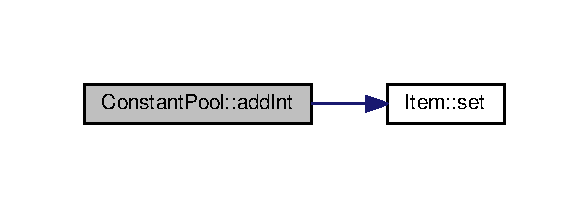
\includegraphics[width=282pt]{classConstantPool_a9f10ea2eb79969299ff5f7a031309093_cgraph}
\end{center}
\end{figure}


\hypertarget{classConstantPool_ad678172b62e701905e72c2cdc72d09a6}{\index{Constant\-Pool@{Constant\-Pool}!add\-Long@{add\-Long}}
\index{add\-Long@{add\-Long}!ConstantPool@{Constant\-Pool}}
\subsubsection[{add\-Long}]{\setlength{\rightskip}{0pt plus 5cm}uint16\-\_\-t Constant\-Pool\-::add\-Long (
\begin{DoxyParamCaption}
\item[{int64\-\_\-t}]{value}
\end{DoxyParamCaption}
)}}\label{classConstantPool_ad678172b62e701905e72c2cdc72d09a6}
method to put a long int into the pool 
\begin{DoxyParams}{Parameters}
{\em value} & value to add to pool \\
\hline
\end{DoxyParams}
\begin{DoxyReturn}{Returns}
index of the long intenger in the pool 
\end{DoxyReturn}


Here is the call graph for this function\-:
\nopagebreak
\begin{figure}[H]
\begin{center}
\leavevmode
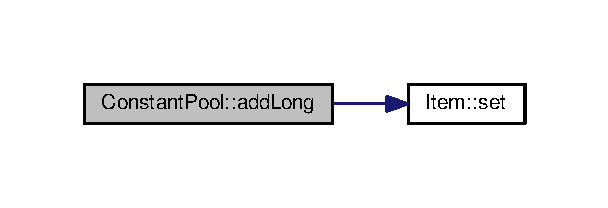
\includegraphics[width=292pt]{classConstantPool_ad678172b62e701905e72c2cdc72d09a6_cgraph}
\end{center}
\end{figure}


\hypertarget{classConstantPool_acecd4913f07d84ff76ac59dee978730d}{\index{Constant\-Pool@{Constant\-Pool}!add\-String@{add\-String}}
\index{add\-String@{add\-String}!ConstantPool@{Constant\-Pool}}
\subsubsection[{add\-String}]{\setlength{\rightskip}{0pt plus 5cm}uint16\-\_\-t Constant\-Pool\-::add\-String (
\begin{DoxyParamCaption}
\item[{const std\-::string \&}]{value}
\end{DoxyParamCaption}
)}}\label{classConstantPool_acecd4913f07d84ff76ac59dee978730d}
method to put a string into the pool 
\begin{DoxyParams}{Parameters}
{\em value} & value to add to pool \\
\hline
\end{DoxyParams}
\begin{DoxyReturn}{Returns}
index of the string in pool 
\end{DoxyReturn}


Here is the call graph for this function\-:
\nopagebreak
\begin{figure}[H]
\begin{center}
\leavevmode
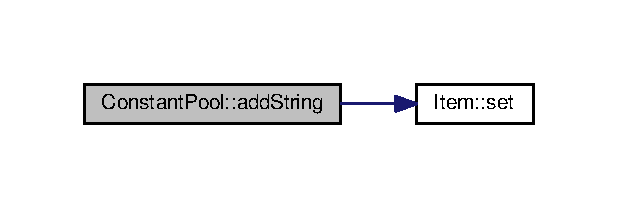
\includegraphics[width=296pt]{classConstantPool_acecd4913f07d84ff76ac59dee978730d_cgraph}
\end{center}
\end{figure}


\hypertarget{classConstantPool_ae37c5a805552c018d71951be2847032a}{\index{Constant\-Pool@{Constant\-Pool}!get\-Byte\-Array@{get\-Byte\-Array}}
\index{get\-Byte\-Array@{get\-Byte\-Array}!ConstantPool@{Constant\-Pool}}
\subsubsection[{get\-Byte\-Array}]{\setlength{\rightskip}{0pt plus 5cm}std\-::vector$<$ uint8\-\_\-t $>$ Constant\-Pool\-::get\-Byte\-Array (
\begin{DoxyParamCaption}
{}
\end{DoxyParamCaption}
)}}\label{classConstantPool_ae37c5a805552c018d71951be2847032a}
returns constant pool as a byte array \begin{DoxyReturn}{Returns}
the bytecode 
\end{DoxyReturn}


The documentation for this class was generated from the following files\-:\begin{DoxyCompactItemize}
\item 
backend/classfile/\hyperlink{constant__pool_8h}{constant\-\_\-pool.\-h}\item 
backend/classfile/\hyperlink{constant__pool_8cc}{constant\-\_\-pool.\-cc}\end{DoxyCompactItemize}

\hypertarget{classGraph}{\section{Graph Class Reference}
\label{classGraph}\index{Graph@{Graph}}
}


{\ttfamily \#include $<$ast.\-h$>$}



Inheritance diagram for Graph\-:
\nopagebreak
\begin{figure}[H]
\begin{center}
\leavevmode
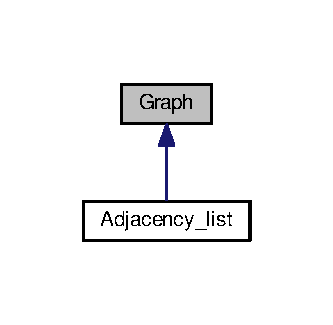
\includegraphics[width=160pt]{classGraph__inherit__graph}
\end{center}
\end{figure}
\subsection*{Public Member Functions}
\begin{DoxyCompactItemize}
\item 
virtual \hyperlink{classGraph_a1621cd1ffcf6a135cbc7e039c305627b}{$\sim$\-Graph} ()
\item 
virtual void \hyperlink{classGraph_ae4ad7e42e8df191acd6563ca65ee779c}{add\-Node} (std\-::shared\-\_\-ptr$<$ \hyperlink{structNode}{Node} $>$ node)=0
\item 
virtual void \hyperlink{classGraph_a9e45aafa60a807245e24565baea74a39}{add\-Edge} (std\-::shared\-\_\-ptr$<$ \hyperlink{structNode}{Node} $>$ source, std\-::shared\-\_\-ptr$<$ \hyperlink{structNode}{Node} $>$ dist, bool path)=0
\item 
virtual std\-::shared\-\_\-ptr$<$ \hyperlink{structNode}{Node} $>$ \hyperlink{classGraph_a7b0c57d46c652fb12e4ca65a816f7a36}{start} ()=0
\item 
virtual std\-::size\-\_\-t \hyperlink{classGraph_afed2883e765871cc439b08d9aeba028b}{node\-Count} () const =0
\item 
virtual std\-::shared\-\_\-ptr$<$ \hyperlink{structNode}{Node} $>$ \hyperlink{classGraph_aa37e2e2fd8d7ae9a94d4e174980644c6}{find} (int id) const =0
\item 
virtual std\-::string \hyperlink{classGraph_a0d1bc2d4425ddbef019b5d7589765c5a}{name} () const =0
\end{DoxyCompactItemize}


\subsection{Detailed Description}
The interface of the \mbox{[}a\mbox{]}bstract \mbox{[}s\mbox{]}yntax \mbox{[}g\mbox{]}raph (A\-S\-G), which consists of different nodes these are representing the commands of the Rail programm. An A\-S\-G represents a function in a Rail programm, that means for each function in a Rail programm there exists a \hyperlink{classGraph}{Graph}.

\begin{DoxyAuthor}{Author}
Christopher Zell \href{mailto:Zelldon91@googlemail.com}{\tt Zelldon91@googlemail.\-com}, Hanin Halawani 
\end{DoxyAuthor}


\subsection{Constructor \& Destructor Documentation}
\hypertarget{classGraph_a1621cd1ffcf6a135cbc7e039c305627b}{\index{Graph@{Graph}!$\sim$\-Graph@{$\sim$\-Graph}}
\index{$\sim$\-Graph@{$\sim$\-Graph}!Graph@{Graph}}
\subsubsection[{$\sim$\-Graph}]{\setlength{\rightskip}{0pt plus 5cm}virtual Graph\-::$\sim$\-Graph (
\begin{DoxyParamCaption}
{}
\end{DoxyParamCaption}
)\hspace{0.3cm}{\ttfamily [inline]}, {\ttfamily [virtual]}}}\label{classGraph_a1621cd1ffcf6a135cbc7e039c305627b}
The destructor of the A\-S\-G. 

\subsection{Member Function Documentation}
\hypertarget{classGraph_a9e45aafa60a807245e24565baea74a39}{\index{Graph@{Graph}!add\-Edge@{add\-Edge}}
\index{add\-Edge@{add\-Edge}!Graph@{Graph}}
\subsubsection[{add\-Edge}]{\setlength{\rightskip}{0pt plus 5cm}virtual void Graph\-::add\-Edge (
\begin{DoxyParamCaption}
\item[{std\-::shared\-\_\-ptr$<$ {\bf Node} $>$}]{source, }
\item[{std\-::shared\-\_\-ptr$<$ {\bf Node} $>$}]{dist, }
\item[{bool}]{path}
\end{DoxyParamCaption}
)\hspace{0.3cm}{\ttfamily [pure virtual]}}}\label{classGraph_a9e45aafa60a807245e24565baea74a39}
Replaces the successor of a certain node. If the path is true the successor1 of the source will be replaced, successor2 if the path is false.


\begin{DoxyParams}{Parameters}
{\em source} & the node which gets a new succesor \\
\hline
{\em dist} & the new successor of the source \\
\hline
{\em path} & specifies whether the successor1 or 2 are been replaced \\
\hline
\end{DoxyParams}


Implemented in \hyperlink{classAdjacency__list_a43a6325bc1e122a2675c39ea826f5f2a}{Adjacency\-\_\-list}.

\hypertarget{classGraph_ae4ad7e42e8df191acd6563ca65ee779c}{\index{Graph@{Graph}!add\-Node@{add\-Node}}
\index{add\-Node@{add\-Node}!Graph@{Graph}}
\subsubsection[{add\-Node}]{\setlength{\rightskip}{0pt plus 5cm}virtual void Graph\-::add\-Node (
\begin{DoxyParamCaption}
\item[{std\-::shared\-\_\-ptr$<$ {\bf Node} $>$}]{node}
\end{DoxyParamCaption}
)\hspace{0.3cm}{\ttfamily [pure virtual]}}}\label{classGraph_ae4ad7e42e8df191acd6563ca65ee779c}
Adds a node (command) to the corresponding A\-S\-G.


\begin{DoxyParams}{Parameters}
{\em node} & the node which will be added \\
\hline
\end{DoxyParams}


Implemented in \hyperlink{classAdjacency__list_adbc9e5768336f17f7442638e5284f2a7}{Adjacency\-\_\-list}.

\hypertarget{classGraph_aa37e2e2fd8d7ae9a94d4e174980644c6}{\index{Graph@{Graph}!find@{find}}
\index{find@{find}!Graph@{Graph}}
\subsubsection[{find}]{\setlength{\rightskip}{0pt plus 5cm}virtual std\-::shared\-\_\-ptr$<${\bf Node}$>$ Graph\-::find (
\begin{DoxyParamCaption}
\item[{int}]{id}
\end{DoxyParamCaption}
) const\hspace{0.3cm}{\ttfamily [pure virtual]}}}\label{classGraph_aa37e2e2fd8d7ae9a94d4e174980644c6}
Finds for the given id the node in the A\-S\-G. 
\begin{DoxyParams}{Parameters}
{\em id} & the id of the node, which should be founded \\
\hline
\end{DoxyParams}
\begin{DoxyReturn}{Returns}
the node with the searched id 
\end{DoxyReturn}


Implemented in \hyperlink{classAdjacency__list_aa15c2f8c06d2d3eee4e2f04002b728ab}{Adjacency\-\_\-list}.

\hypertarget{classGraph_a0d1bc2d4425ddbef019b5d7589765c5a}{\index{Graph@{Graph}!name@{name}}
\index{name@{name}!Graph@{Graph}}
\subsubsection[{name}]{\setlength{\rightskip}{0pt plus 5cm}virtual std\-::string Graph\-::name (
\begin{DoxyParamCaption}
{}
\end{DoxyParamCaption}
) const\hspace{0.3cm}{\ttfamily [pure virtual]}}}\label{classGraph_a0d1bc2d4425ddbef019b5d7589765c5a}
Returns the name of the A\-S\-G. The name of the graph is equal to the name of the Rail function. (Each function has his own graph) \begin{DoxyReturn}{Returns}
the name of the A\-S\-G 
\end{DoxyReturn}


Implemented in \hyperlink{classAdjacency__list_ab2eea0405522e8b9917d84ef44e70f66}{Adjacency\-\_\-list}.

\hypertarget{classGraph_afed2883e765871cc439b08d9aeba028b}{\index{Graph@{Graph}!node\-Count@{node\-Count}}
\index{node\-Count@{node\-Count}!Graph@{Graph}}
\subsubsection[{node\-Count}]{\setlength{\rightskip}{0pt plus 5cm}virtual std\-::size\-\_\-t Graph\-::node\-Count (
\begin{DoxyParamCaption}
{}
\end{DoxyParamCaption}
) const\hspace{0.3cm}{\ttfamily [pure virtual]}}}\label{classGraph_afed2883e765871cc439b08d9aeba028b}
Returns the current size of the graph (node count). \begin{DoxyReturn}{Returns}
the size of the A\-S\-G 
\end{DoxyReturn}


Implemented in \hyperlink{classAdjacency__list_ac67e271d3a734fc596d678490101b509}{Adjacency\-\_\-list}.

\hypertarget{classGraph_a7b0c57d46c652fb12e4ca65a816f7a36}{\index{Graph@{Graph}!start@{start}}
\index{start@{start}!Graph@{Graph}}
\subsubsection[{start}]{\setlength{\rightskip}{0pt plus 5cm}virtual std\-::shared\-\_\-ptr$<${\bf Node}$>$ Graph\-::start (
\begin{DoxyParamCaption}
{}
\end{DoxyParamCaption}
)\hspace{0.3cm}{\ttfamily [pure virtual]}}}\label{classGraph_a7b0c57d46c652fb12e4ca65a816f7a36}
Returns the start node of the A\-S\-G, respectively of the Rail function. \begin{DoxyReturn}{Returns}
the start node 
\end{DoxyReturn}


Implemented in \hyperlink{classAdjacency__list_a129aec8db0fc3b6109de60f765c41ac4}{Adjacency\-\_\-list}.



The documentation for this class was generated from the following file\-:\begin{DoxyCompactItemize}
\item 
common/ast/\hyperlink{ast_8h}{ast.\-h}\end{DoxyCompactItemize}

\hypertarget{classGraphs}{\section{Graphs Class Reference}
\label{classGraphs}\index{Graphs@{Graphs}}
}


{\ttfamily \#include $<$Graphs.\-h$>$}

\subsection*{Public Types}
\begin{DoxyCompactItemize}
\item 
typedef std\-::shared\-\_\-ptr$<$ \hyperlink{structNode}{Node} $>$ \hyperlink{classGraphs_a2804b752d72989344f11a6ec3145eea8}{Node\-\_\-ptr}
\item 
typedef std\-::shared\-\_\-ptr$<$ \hyperlink{classGraph}{Graph} $>$ \hyperlink{classGraphs_a58b4b65d81870fc3b2936c068b644a4d}{Graph\-\_\-ptr}
\item 
typedef std\-::map$<$ std\-::string, \\*
\hyperlink{classGraphs_a58b4b65d81870fc3b2936c068b644a4d}{Graph\-\_\-ptr} $>$ \hyperlink{classGraphs_ae84f43c27f4abeec92270c954a9255d4}{Graph\-\_\-map}
\item 
typedef const std\-::string \& \hyperlink{classGraphs_a98a6f0415cbeae8adc7500164c78e3f3}{str}
\end{DoxyCompactItemize}
\subsection*{Public Member Functions}
\begin{DoxyCompactItemize}
\item 
\hyperlink{classGraphs_ac474b1dea2e194dd74f554e75d60b83a}{Graphs} ()
\item 
virtual \hyperlink{classGraphs_ad1f81a7661844de33fc248c8575c9d3e}{$\sim$\-Graphs} ()
\item 
virtual bool \hyperlink{classGraphs_a4918b1f853cb695103da70945f8fd431}{put} (\hyperlink{classGraphs_a98a6f0415cbeae8adc7500164c78e3f3}{str} key, \hyperlink{classGraphs_a58b4b65d81870fc3b2936c068b644a4d}{Graph\-\_\-ptr} graph)
\item 
virtual \hyperlink{classGraphs_a58b4b65d81870fc3b2936c068b644a4d}{Graph\-\_\-ptr} \hyperlink{classGraphs_a91dad024134f39c0695017b419bc5e30}{find} (\hyperlink{classGraphs_a98a6f0415cbeae8adc7500164c78e3f3}{str} key)
\item 
virtual Graph\-\_\-map\-::iterator \hyperlink{classGraphs_a8a073cce4572a581991904bdf3fe08cc}{begin} ()
\item 
virtual Graph\-\_\-map\-::iterator \hyperlink{classGraphs_a0e29872711f39db4c244dd1bf970b298}{end} ()
\item 
virtual size\-\_\-t \hyperlink{classGraphs_a3b054630d2bf941bcb7f27f6b4af7830}{size} ()
\item 
virtual void \hyperlink{classGraphs_a50f10866f91655a7159aa4fe4abb66dd}{marshall} (\hyperlink{classGraphs_a98a6f0415cbeae8adc7500164c78e3f3}{str} file)
\item 
virtual void \hyperlink{classGraphs_ae16cf56023c83cd77e8b5592c9274c5f}{unmarshall} (\hyperlink{classGraphs_a98a6f0415cbeae8adc7500164c78e3f3}{str} file, char delimeter)
\item 
void \hyperlink{classGraphs_a6a93fd87235a675d39c23e8fcbafb8b1}{write\-Graph\-Viz} (\hyperlink{classGraphs_a98a6f0415cbeae8adc7500164c78e3f3}{Graphs\-::str} file)
\end{DoxyCompactItemize}


\subsection{Member Typedef Documentation}
\hypertarget{classGraphs_ae84f43c27f4abeec92270c954a9255d4}{\index{Graphs@{Graphs}!Graph\-\_\-map@{Graph\-\_\-map}}
\index{Graph\-\_\-map@{Graph\-\_\-map}!Graphs@{Graphs}}
\subsubsection[{Graph\-\_\-map}]{\setlength{\rightskip}{0pt plus 5cm}typedef std\-::map$<$std\-::string, {\bf Graph\-\_\-ptr}$>$ {\bf Graphs\-::\-Graph\-\_\-map}}}\label{classGraphs_ae84f43c27f4abeec92270c954a9255d4}
\hypertarget{classGraphs_a58b4b65d81870fc3b2936c068b644a4d}{\index{Graphs@{Graphs}!Graph\-\_\-ptr@{Graph\-\_\-ptr}}
\index{Graph\-\_\-ptr@{Graph\-\_\-ptr}!Graphs@{Graphs}}
\subsubsection[{Graph\-\_\-ptr}]{\setlength{\rightskip}{0pt plus 5cm}typedef std\-::shared\-\_\-ptr$<${\bf Graph}$>$ {\bf Graphs\-::\-Graph\-\_\-ptr}}}\label{classGraphs_a58b4b65d81870fc3b2936c068b644a4d}
\hypertarget{classGraphs_a2804b752d72989344f11a6ec3145eea8}{\index{Graphs@{Graphs}!Node\-\_\-ptr@{Node\-\_\-ptr}}
\index{Node\-\_\-ptr@{Node\-\_\-ptr}!Graphs@{Graphs}}
\subsubsection[{Node\-\_\-ptr}]{\setlength{\rightskip}{0pt plus 5cm}typedef std\-::shared\-\_\-ptr$<${\bf Node}$>$ {\bf Graphs\-::\-Node\-\_\-ptr}}}\label{classGraphs_a2804b752d72989344f11a6ec3145eea8}
\hypertarget{classGraphs_a98a6f0415cbeae8adc7500164c78e3f3}{\index{Graphs@{Graphs}!str@{str}}
\index{str@{str}!Graphs@{Graphs}}
\subsubsection[{str}]{\setlength{\rightskip}{0pt plus 5cm}typedef const std\-::string\& {\bf Graphs\-::str}}}\label{classGraphs_a98a6f0415cbeae8adc7500164c78e3f3}


\subsection{Constructor \& Destructor Documentation}
\hypertarget{classGraphs_ac474b1dea2e194dd74f554e75d60b83a}{\index{Graphs@{Graphs}!Graphs@{Graphs}}
\index{Graphs@{Graphs}!Graphs@{Graphs}}
\subsubsection[{Graphs}]{\setlength{\rightskip}{0pt plus 5cm}Graphs\-::\-Graphs (
\begin{DoxyParamCaption}
{}
\end{DoxyParamCaption}
)}}\label{classGraphs_ac474b1dea2e194dd74f554e75d60b83a}
\hypertarget{classGraphs_ad1f81a7661844de33fc248c8575c9d3e}{\index{Graphs@{Graphs}!$\sim$\-Graphs@{$\sim$\-Graphs}}
\index{$\sim$\-Graphs@{$\sim$\-Graphs}!Graphs@{Graphs}}
\subsubsection[{$\sim$\-Graphs}]{\setlength{\rightskip}{0pt plus 5cm}Graphs\-::$\sim$\-Graphs (
\begin{DoxyParamCaption}
{}
\end{DoxyParamCaption}
)\hspace{0.3cm}{\ttfamily [virtual]}}}\label{classGraphs_ad1f81a7661844de33fc248c8575c9d3e}


\subsection{Member Function Documentation}
\hypertarget{classGraphs_a8a073cce4572a581991904bdf3fe08cc}{\index{Graphs@{Graphs}!begin@{begin}}
\index{begin@{begin}!Graphs@{Graphs}}
\subsubsection[{begin}]{\setlength{\rightskip}{0pt plus 5cm}Graphs\-::\-Graph\-\_\-map\-::iterator Graphs\-::begin (
\begin{DoxyParamCaption}
{}
\end{DoxyParamCaption}
)\hspace{0.3cm}{\ttfamily [virtual]}}}\label{classGraphs_a8a073cce4572a581991904bdf3fe08cc}
\hypertarget{classGraphs_a0e29872711f39db4c244dd1bf970b298}{\index{Graphs@{Graphs}!end@{end}}
\index{end@{end}!Graphs@{Graphs}}
\subsubsection[{end}]{\setlength{\rightskip}{0pt plus 5cm}Graphs\-::\-Graph\-\_\-map\-::iterator Graphs\-::end (
\begin{DoxyParamCaption}
{}
\end{DoxyParamCaption}
)\hspace{0.3cm}{\ttfamily [virtual]}}}\label{classGraphs_a0e29872711f39db4c244dd1bf970b298}
\hypertarget{classGraphs_a91dad024134f39c0695017b419bc5e30}{\index{Graphs@{Graphs}!find@{find}}
\index{find@{find}!Graphs@{Graphs}}
\subsubsection[{find}]{\setlength{\rightskip}{0pt plus 5cm}{\bf Graphs\-::\-Graph\-\_\-ptr} Graphs\-::find (
\begin{DoxyParamCaption}
\item[{{\bf Graphs\-::str}}]{key}
\end{DoxyParamCaption}
)\hspace{0.3cm}{\ttfamily [virtual]}}}\label{classGraphs_a91dad024134f39c0695017b419bc5e30}
\hypertarget{classGraphs_a50f10866f91655a7159aa4fe4abb66dd}{\index{Graphs@{Graphs}!marshall@{marshall}}
\index{marshall@{marshall}!Graphs@{Graphs}}
\subsubsection[{marshall}]{\setlength{\rightskip}{0pt plus 5cm}void Graphs\-::marshall (
\begin{DoxyParamCaption}
\item[{{\bf Graphs\-::str}}]{file}
\end{DoxyParamCaption}
)\hspace{0.3cm}{\ttfamily [virtual]}}}\label{classGraphs_a50f10866f91655a7159aa4fe4abb66dd}


Here is the call graph for this function\-:
\nopagebreak
\begin{figure}[H]
\begin{center}
\leavevmode
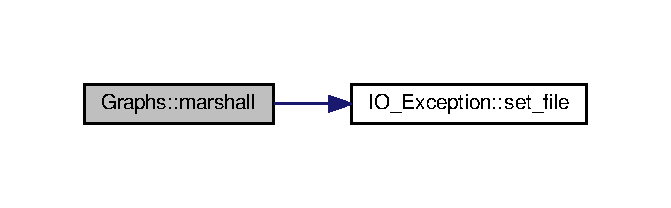
\includegraphics[width=322pt]{classGraphs_a50f10866f91655a7159aa4fe4abb66dd_cgraph}
\end{center}
\end{figure}


\hypertarget{classGraphs_a4918b1f853cb695103da70945f8fd431}{\index{Graphs@{Graphs}!put@{put}}
\index{put@{put}!Graphs@{Graphs}}
\subsubsection[{put}]{\setlength{\rightskip}{0pt plus 5cm}bool Graphs\-::put (
\begin{DoxyParamCaption}
\item[{{\bf Graphs\-::str}}]{key, }
\item[{{\bf Graphs\-::\-Graph\-\_\-ptr}}]{graph}
\end{DoxyParamCaption}
)\hspace{0.3cm}{\ttfamily [virtual]}}}\label{classGraphs_a4918b1f853cb695103da70945f8fd431}
\hypertarget{classGraphs_a3b054630d2bf941bcb7f27f6b4af7830}{\index{Graphs@{Graphs}!size@{size}}
\index{size@{size}!Graphs@{Graphs}}
\subsubsection[{size}]{\setlength{\rightskip}{0pt plus 5cm}size\-\_\-t Graphs\-::size (
\begin{DoxyParamCaption}
{}
\end{DoxyParamCaption}
)\hspace{0.3cm}{\ttfamily [virtual]}}}\label{classGraphs_a3b054630d2bf941bcb7f27f6b4af7830}
\hypertarget{classGraphs_ae16cf56023c83cd77e8b5592c9274c5f}{\index{Graphs@{Graphs}!unmarshall@{unmarshall}}
\index{unmarshall@{unmarshall}!Graphs@{Graphs}}
\subsubsection[{unmarshall}]{\setlength{\rightskip}{0pt plus 5cm}void Graphs\-::unmarshall (
\begin{DoxyParamCaption}
\item[{{\bf Graphs\-::str}}]{file, }
\item[{char}]{delimeter}
\end{DoxyParamCaption}
)\hspace{0.3cm}{\ttfamily [virtual]}}}\label{classGraphs_ae16cf56023c83cd77e8b5592c9274c5f}


Here is the call graph for this function\-:
\nopagebreak
\begin{figure}[H]
\begin{center}
\leavevmode
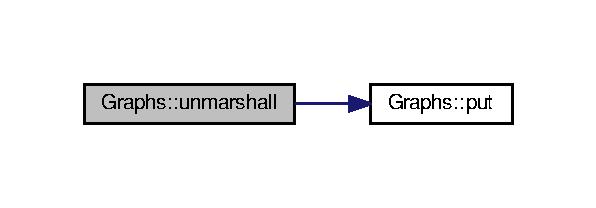
\includegraphics[width=286pt]{classGraphs_ae16cf56023c83cd77e8b5592c9274c5f_cgraph}
\end{center}
\end{figure}


\hypertarget{classGraphs_a6a93fd87235a675d39c23e8fcbafb8b1}{\index{Graphs@{Graphs}!write\-Graph\-Viz@{write\-Graph\-Viz}}
\index{write\-Graph\-Viz@{write\-Graph\-Viz}!Graphs@{Graphs}}
\subsubsection[{write\-Graph\-Viz}]{\setlength{\rightskip}{0pt plus 5cm}void Graphs\-::write\-Graph\-Viz (
\begin{DoxyParamCaption}
\item[{{\bf Graphs\-::str}}]{file}
\end{DoxyParamCaption}
)}}\label{classGraphs_a6a93fd87235a675d39c23e8fcbafb8b1}


Here is the call graph for this function\-:
\nopagebreak
\begin{figure}[H]
\begin{center}
\leavevmode
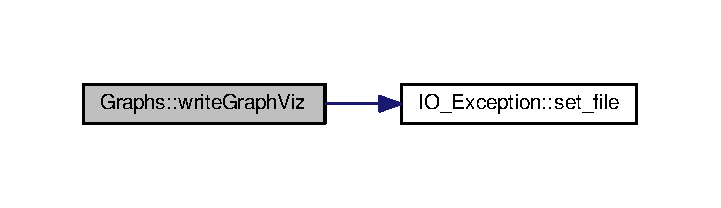
\includegraphics[width=346pt]{classGraphs_a6a93fd87235a675d39c23e8fcbafb8b1_cgraph}
\end{center}
\end{figure}




The documentation for this class was generated from the following files\-:\begin{DoxyCompactItemize}
\item 
frontend/\hyperlink{Graphs_8h}{Graphs.\-h}\item 
frontend/\hyperlink{Graphs_8cpp}{Graphs.\-cpp}\end{DoxyCompactItemize}

\hypertarget{classInvalid__Format__Exception}{\section{Invalid\-\_\-\-Format\-\_\-\-Exception Class Reference}
\label{classInvalid__Format__Exception}\index{Invalid\-\_\-\-Format\-\_\-\-Exception@{Invalid\-\_\-\-Format\-\_\-\-Exception}}
}


{\ttfamily \#include $<$Invalid\-\_\-\-Format\-\_\-\-Exception.\-h$>$}



Inheritance diagram for Invalid\-\_\-\-Format\-\_\-\-Exception\-:
\nopagebreak
\begin{figure}[H]
\begin{center}
\leavevmode
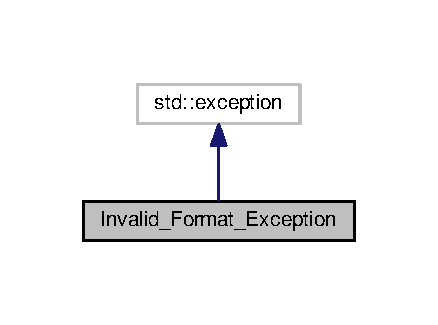
\includegraphics[width=210pt]{classInvalid__Format__Exception__inherit__graph}
\end{center}
\end{figure}


Collaboration diagram for Invalid\-\_\-\-Format\-\_\-\-Exception\-:
\nopagebreak
\begin{figure}[H]
\begin{center}
\leavevmode
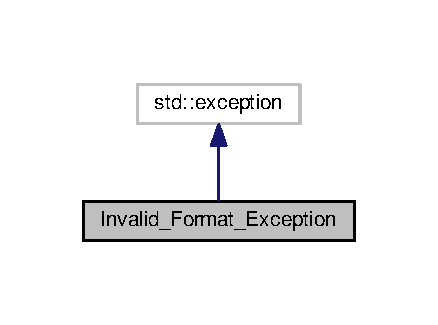
\includegraphics[width=210pt]{classInvalid__Format__Exception__coll__graph}
\end{center}
\end{figure}


The documentation for this class was generated from the following file\-:\begin{DoxyCompactItemize}
\item 
frontend/\hyperlink{Invalid__Format__Exception_8h}{Invalid\-\_\-\-Format\-\_\-\-Exception.\-h}\end{DoxyCompactItemize}

\hypertarget{classIO__Exception}{\section{I\-O\-\_\-\-Exception Class Reference}
\label{classIO__Exception}\index{I\-O\-\_\-\-Exception@{I\-O\-\_\-\-Exception}}
}


{\ttfamily \#include $<$I\-O\-\_\-\-Exception.\-h$>$}



Inheritance diagram for I\-O\-\_\-\-Exception\-:
\nopagebreak
\begin{figure}[H]
\begin{center}
\leavevmode
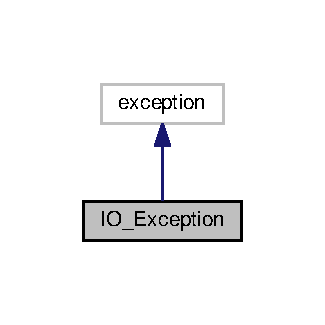
\includegraphics[width=156pt]{classIO__Exception__inherit__graph}
\end{center}
\end{figure}


Collaboration diagram for I\-O\-\_\-\-Exception\-:
\nopagebreak
\begin{figure}[H]
\begin{center}
\leavevmode
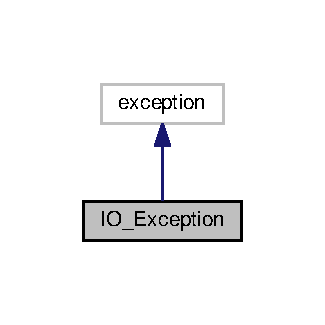
\includegraphics[width=156pt]{classIO__Exception__coll__graph}
\end{center}
\end{figure}
\subsection*{Public Member Functions}
\begin{DoxyCompactItemize}
\item 
void \hyperlink{classIO__Exception_a2a30b4efa90ca4cd554bab9da920ec63}{set\-\_\-file} (const std\-::string \&file\-Name)
\end{DoxyCompactItemize}


\subsection{Member Function Documentation}
\hypertarget{classIO__Exception_a2a30b4efa90ca4cd554bab9da920ec63}{\index{I\-O\-\_\-\-Exception@{I\-O\-\_\-\-Exception}!set\-\_\-file@{set\-\_\-file}}
\index{set\-\_\-file@{set\-\_\-file}!IO_Exception@{I\-O\-\_\-\-Exception}}
\subsubsection[{set\-\_\-file}]{\setlength{\rightskip}{0pt plus 5cm}void I\-O\-\_\-\-Exception\-::set\-\_\-file (
\begin{DoxyParamCaption}
\item[{const std\-::string \&}]{file\-Name}
\end{DoxyParamCaption}
)\hspace{0.3cm}{\ttfamily [inline]}}}\label{classIO__Exception_a2a30b4efa90ca4cd554bab9da920ec63}


The documentation for this class was generated from the following file\-:\begin{DoxyCompactItemize}
\item 
frontend/\hyperlink{IO__Exception_8h}{I\-O\-\_\-\-Exception.\-h}\end{DoxyCompactItemize}

\hypertarget{classItem}{\section{Item Class Reference}
\label{classItem}\index{Item@{Item}}
}


{\ttfamily \#include $<$constant\-\_\-pool.\-h$>$}



Collaboration diagram for Item\-:
\nopagebreak
\begin{figure}[H]
\begin{center}
\leavevmode
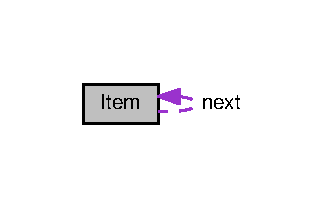
\includegraphics[width=156pt]{classItem__coll__graph}
\end{center}
\end{figure}
\subsection*{Public Member Functions}
\begin{DoxyCompactItemize}
\item 
\hyperlink{classItem_a297720c02984eab37332ae795d22189d}{Item} ()
\begin{DoxyCompactList}\small\item\em default constructor does nothing, bud is needed because we have other \end{DoxyCompactList}\item 
\hyperlink{classItem_ade7e491f0f1fb579f98c28f7079ace05}{Item} (const \hyperlink{classItem}{Item} \&i)
\item 
\hyperlink{classItem_a67f7e880e22f809d8d79cf506f5b2cda}{Item} (uint16\-\_\-t \-\_\-index)
\item 
\hyperlink{classItem_ac10ca71346b926c98fd3084009d59631}{Item} (uint16\-\_\-t \-\_\-index, const \hyperlink{classItem}{Item} \&i)
\item 
bool \hyperlink{classItem_a84846489b45c30f17e16a2dc2b67b3ce}{operator==} (const \hyperlink{classItem}{Item} \&i) const 
\item 
bool \hyperlink{classItem_a007f803456c6eb508b58539546181722}{operator=} (const \hyperlink{classItem}{Item} \&i)
\item 
void \hyperlink{classItem_a6c9c2df6f8e7e5bd6816cbbb9d50bf1e}{set} (int32\-\_\-t \hyperlink{classItem_a37e64449e06749eded7f699b13f8ede7}{int\-Val})
\item 
void \hyperlink{classItem_a778afe86a8bae9e56686e153b4550460}{set} (int64\-\_\-t \hyperlink{classItem_aaaa7f2c4f4a2163862b1508202ecf038}{long\-Val})
\item 
void \hyperlink{classItem_a0a4eb862c72e765ee779e3c461bfdcc0}{set} (int32\-\_\-t \-\_\-type, const std\-::string \&\-\_\-str\-Val1, const std\-::string \&\-\_\-str\-Val2, const std\-::string \&\-\_\-str\-Val3)
\end{DoxyCompactItemize}
\subsection*{Public Attributes}
\begin{DoxyCompactItemize}
\item 
\hyperlink{classItem}{Item} $\ast$ \hyperlink{classItem_af41ed24b86b2126cf7eacc591a863f47}{next}
\item 
uint16\-\_\-t \hyperlink{classItem_aee551f9d28c1aef4bd3b15e9dfe5f6fd}{index}
\item 
int32\-\_\-t \hyperlink{classItem_ad16d911a86476ef205aaa08dbc0af182}{type}
\item 
int32\-\_\-t \hyperlink{classItem_a37e64449e06749eded7f699b13f8ede7}{int\-Val}
\item 
int64\-\_\-t \hyperlink{classItem_aaaa7f2c4f4a2163862b1508202ecf038}{long\-Val}
\item 
std\-::string \hyperlink{classItem_a0769fc287f38f56be204b2deb9fc9326}{str\-Val1}
\item 
std\-::string \hyperlink{classItem_a44fde30371f8000e026420c69ed37236}{str\-Val2}
\item 
std\-::string \hyperlink{classItem_ae1567b4fa0100b38469c1cdef4c705d2}{str\-Val3}
\item 
int32\-\_\-t \hyperlink{classItem_a1fad09954d2cc9ec2233d3328aead6c2}{hash\-Code}
\end{DoxyCompactItemize}


\subsection{Constructor \& Destructor Documentation}
\hypertarget{classItem_a297720c02984eab37332ae795d22189d}{\index{Item@{Item}!Item@{Item}}
\index{Item@{Item}!Item@{Item}}
\subsubsection[{Item}]{\setlength{\rightskip}{0pt plus 5cm}Item\-::\-Item (
\begin{DoxyParamCaption}
{}
\end{DoxyParamCaption}
)}}\label{classItem_a297720c02984eab37332ae795d22189d}


default constructor does nothing, bud is needed because we have other 

\hypertarget{classItem_ade7e491f0f1fb579f98c28f7079ace05}{\index{Item@{Item}!Item@{Item}}
\index{Item@{Item}!Item@{Item}}
\subsubsection[{Item}]{\setlength{\rightskip}{0pt plus 5cm}Item\-::\-Item (
\begin{DoxyParamCaption}
\item[{const {\bf Item} \&}]{i}
\end{DoxyParamCaption}
)\hspace{0.3cm}{\ttfamily [explicit]}}}\label{classItem_ade7e491f0f1fb579f98c28f7079ace05}
copy constructor 
\begin{DoxyParams}{Parameters}
{\em i} & item with values to set to \\
\hline
\end{DoxyParams}
\hypertarget{classItem_a67f7e880e22f809d8d79cf506f5b2cda}{\index{Item@{Item}!Item@{Item}}
\index{Item@{Item}!Item@{Item}}
\subsubsection[{Item}]{\setlength{\rightskip}{0pt plus 5cm}Item\-::\-Item (
\begin{DoxyParamCaption}
\item[{uint16\-\_\-t}]{\-\_\-index}
\end{DoxyParamCaption}
)\hspace{0.3cm}{\ttfamily [explicit]}}}\label{classItem_a67f7e880e22f809d8d79cf506f5b2cda}
constructor with defined index 
\begin{DoxyParams}{Parameters}
{\em index} & internal index of item \\
\hline
\end{DoxyParams}
\hypertarget{classItem_ac10ca71346b926c98fd3084009d59631}{\index{Item@{Item}!Item@{Item}}
\index{Item@{Item}!Item@{Item}}
\subsubsection[{Item}]{\setlength{\rightskip}{0pt plus 5cm}Item\-::\-Item (
\begin{DoxyParamCaption}
\item[{uint16\-\_\-t}]{\-\_\-index, }
\item[{const {\bf Item} \&}]{i}
\end{DoxyParamCaption}
)}}\label{classItem_ac10ca71346b926c98fd3084009d59631}
constructor 
\begin{DoxyParams}{Parameters}
{\em \-\_\-index} & internal index \\
\hline
{\em i} & item to set to \\
\hline
\end{DoxyParams}


\subsection{Member Function Documentation}
\hypertarget{classItem_a007f803456c6eb508b58539546181722}{\index{Item@{Item}!operator=@{operator=}}
\index{operator=@{operator=}!Item@{Item}}
\subsubsection[{operator=}]{\setlength{\rightskip}{0pt plus 5cm}bool Item\-::operator= (
\begin{DoxyParamCaption}
\item[{const {\bf Item} \&}]{i}
\end{DoxyParamCaption}
)}}\label{classItem_a007f803456c6eb508b58539546181722}
copy operator 
\begin{DoxyParams}{Parameters}
{\em i} & item to be copied \\
\hline
\end{DoxyParams}
\hypertarget{classItem_a84846489b45c30f17e16a2dc2b67b3ce}{\index{Item@{Item}!operator==@{operator==}}
\index{operator==@{operator==}!Item@{Item}}
\subsubsection[{operator==}]{\setlength{\rightskip}{0pt plus 5cm}bool Item\-::operator== (
\begin{DoxyParamCaption}
\item[{const {\bf Item} \&}]{i}
\end{DoxyParamCaption}
) const}}\label{classItem_a84846489b45c30f17e16a2dc2b67b3ce}
compare operator implementation 
\begin{DoxyParams}{Parameters}
{\em i} & copmared item \\
\hline
\end{DoxyParams}
\hypertarget{classItem_a6c9c2df6f8e7e5bd6816cbbb9d50bf1e}{\index{Item@{Item}!set@{set}}
\index{set@{set}!Item@{Item}}
\subsubsection[{set}]{\setlength{\rightskip}{0pt plus 5cm}void Item\-::set (
\begin{DoxyParamCaption}
\item[{int32\-\_\-t}]{\-\_\-int\-Val}
\end{DoxyParamCaption}
)}}\label{classItem_a6c9c2df6f8e7e5bd6816cbbb9d50bf1e}
set item to integer value 
\begin{DoxyParams}{Parameters}
{\em \-\_\-int\-Val} & integer value \\
\hline
\end{DoxyParams}
\hypertarget{classItem_a778afe86a8bae9e56686e153b4550460}{\index{Item@{Item}!set@{set}}
\index{set@{set}!Item@{Item}}
\subsubsection[{set}]{\setlength{\rightskip}{0pt plus 5cm}void Item\-::set (
\begin{DoxyParamCaption}
\item[{int64\-\_\-t}]{\-\_\-long\-Val}
\end{DoxyParamCaption}
)}}\label{classItem_a778afe86a8bae9e56686e153b4550460}
set item to long value 
\begin{DoxyParams}{Parameters}
{\em \-\_\-long\-Val} & long integer value \\
\hline
\end{DoxyParams}
\hypertarget{classItem_a0a4eb862c72e765ee779e3c461bfdcc0}{\index{Item@{Item}!set@{set}}
\index{set@{set}!Item@{Item}}
\subsubsection[{set}]{\setlength{\rightskip}{0pt plus 5cm}void Item\-::set (
\begin{DoxyParamCaption}
\item[{int32\-\_\-t}]{\-\_\-type, }
\item[{const std\-::string \&}]{\-\_\-str\-Val1, }
\item[{const std\-::string \&}]{\-\_\-str\-Val2, }
\item[{const std\-::string \&}]{\-\_\-str\-Val3}
\end{DoxyParamCaption}
)}}\label{classItem_a0a4eb862c72e765ee779e3c461bfdcc0}
set item to string value 
\begin{DoxyParams}{Parameters}
{\em \-\_\-type} & type of the item \\
\hline
{\em \-\_\-str\-Val1} & first part of the value of this item. \\
\hline
{\em \-\_\-str\-Val2} & second part of the value of this item. \\
\hline
{\em \-\_\-str\-Val3} & third part of the value of this item. \\
\hline
\end{DoxyParams}


\subsection{Member Data Documentation}
\hypertarget{classItem_a1fad09954d2cc9ec2233d3328aead6c2}{\index{Item@{Item}!hash\-Code@{hash\-Code}}
\index{hash\-Code@{hash\-Code}!Item@{Item}}
\subsubsection[{hash\-Code}]{\setlength{\rightskip}{0pt plus 5cm}int32\-\_\-t Item\-::hash\-Code}}\label{classItem_a1fad09954d2cc9ec2233d3328aead6c2}
\hypertarget{classItem_aee551f9d28c1aef4bd3b15e9dfe5f6fd}{\index{Item@{Item}!index@{index}}
\index{index@{index}!Item@{Item}}
\subsubsection[{index}]{\setlength{\rightskip}{0pt plus 5cm}uint16\-\_\-t Item\-::index}}\label{classItem_aee551f9d28c1aef4bd3b15e9dfe5f6fd}
\hypertarget{classItem_a37e64449e06749eded7f699b13f8ede7}{\index{Item@{Item}!int\-Val@{int\-Val}}
\index{int\-Val@{int\-Val}!Item@{Item}}
\subsubsection[{int\-Val}]{\setlength{\rightskip}{0pt plus 5cm}int32\-\_\-t Item\-::int\-Val}}\label{classItem_a37e64449e06749eded7f699b13f8ede7}
\hypertarget{classItem_aaaa7f2c4f4a2163862b1508202ecf038}{\index{Item@{Item}!long\-Val@{long\-Val}}
\index{long\-Val@{long\-Val}!Item@{Item}}
\subsubsection[{long\-Val}]{\setlength{\rightskip}{0pt plus 5cm}int64\-\_\-t Item\-::long\-Val}}\label{classItem_aaaa7f2c4f4a2163862b1508202ecf038}
\hypertarget{classItem_af41ed24b86b2126cf7eacc591a863f47}{\index{Item@{Item}!next@{next}}
\index{next@{next}!Item@{Item}}
\subsubsection[{next}]{\setlength{\rightskip}{0pt plus 5cm}{\bf Item}$\ast$ Item\-::next}}\label{classItem_af41ed24b86b2126cf7eacc591a863f47}
\hypertarget{classItem_a0769fc287f38f56be204b2deb9fc9326}{\index{Item@{Item}!str\-Val1@{str\-Val1}}
\index{str\-Val1@{str\-Val1}!Item@{Item}}
\subsubsection[{str\-Val1}]{\setlength{\rightskip}{0pt plus 5cm}std\-::string Item\-::str\-Val1}}\label{classItem_a0769fc287f38f56be204b2deb9fc9326}
\hypertarget{classItem_a44fde30371f8000e026420c69ed37236}{\index{Item@{Item}!str\-Val2@{str\-Val2}}
\index{str\-Val2@{str\-Val2}!Item@{Item}}
\subsubsection[{str\-Val2}]{\setlength{\rightskip}{0pt plus 5cm}std\-::string Item\-::str\-Val2}}\label{classItem_a44fde30371f8000e026420c69ed37236}
\hypertarget{classItem_ae1567b4fa0100b38469c1cdef4c705d2}{\index{Item@{Item}!str\-Val3@{str\-Val3}}
\index{str\-Val3@{str\-Val3}!Item@{Item}}
\subsubsection[{str\-Val3}]{\setlength{\rightskip}{0pt plus 5cm}std\-::string Item\-::str\-Val3}}\label{classItem_ae1567b4fa0100b38469c1cdef4c705d2}
\hypertarget{classItem_ad16d911a86476ef205aaa08dbc0af182}{\index{Item@{Item}!type@{type}}
\index{type@{type}!Item@{Item}}
\subsubsection[{type}]{\setlength{\rightskip}{0pt plus 5cm}int32\-\_\-t Item\-::type}}\label{classItem_ad16d911a86476ef205aaa08dbc0af182}


The documentation for this class was generated from the following files\-:\begin{DoxyCompactItemize}
\item 
backend/classfile/\hyperlink{constant__pool_8h}{constant\-\_\-pool.\-h}\item 
backend/classfile/\hyperlink{constant__pool_8cc}{constant\-\_\-pool.\-cc}\end{DoxyCompactItemize}

\hypertarget{classLexer}{\section{Lexer Class Reference}
\label{classLexer}\index{Lexer@{Lexer}}
}


{\ttfamily \#include $<$lexer.\-h$>$}

\subsection*{Public Member Functions}
\begin{DoxyCompactItemize}
\item 
void \hyperlink{classLexer_ac67cb8fbc383ddf7a859b29c343fd5a9}{lex} (const string \&filename)
\end{DoxyCompactItemize}
\subsection*{Public Attributes}
\begin{DoxyCompactItemize}
\item 
vector$<$ \hyperlink{classRailFunction}{Rail\-Function} $>$ \hyperlink{classLexer_ad777c9574b2267f65ae9793a5a60c0a8}{functions}
\end{DoxyCompactItemize}


\subsection{Member Function Documentation}
\hypertarget{classLexer_ac67cb8fbc383ddf7a859b29c343fd5a9}{\index{Lexer@{Lexer}!lex@{lex}}
\index{lex@{lex}!Lexer@{Lexer}}
\subsubsection[{lex}]{\setlength{\rightskip}{0pt plus 5cm}void Lexer\-::lex (
\begin{DoxyParamCaption}
\item[{const string \&}]{filename}
\end{DoxyParamCaption}
)}}\label{classLexer_ac67cb8fbc383ddf7a859b29c343fd5a9}


Here is the call graph for this function\-:
\nopagebreak
\begin{figure}[H]
\begin{center}
\leavevmode
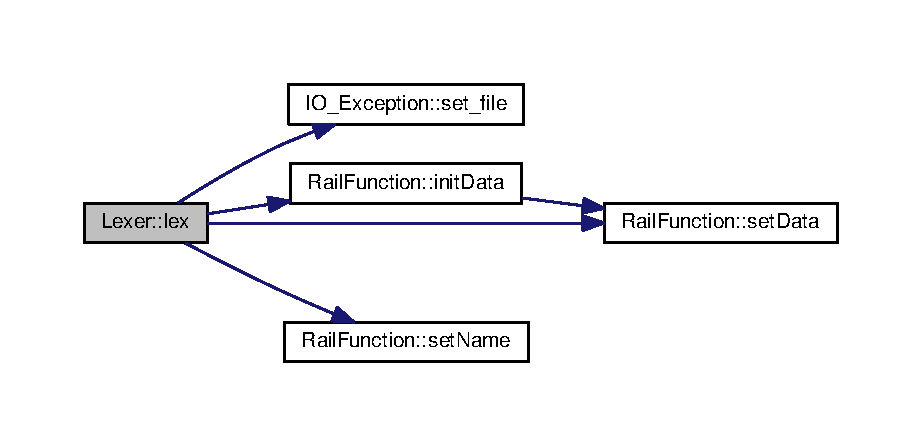
\includegraphics[width=350pt]{classLexer_ac67cb8fbc383ddf7a859b29c343fd5a9_cgraph}
\end{center}
\end{figure}




\subsection{Member Data Documentation}
\hypertarget{classLexer_ad777c9574b2267f65ae9793a5a60c0a8}{\index{Lexer@{Lexer}!functions@{functions}}
\index{functions@{functions}!Lexer@{Lexer}}
\subsubsection[{functions}]{\setlength{\rightskip}{0pt plus 5cm}vector$<${\bf Rail\-Function}$>$ Lexer\-::functions}}\label{classLexer_ad777c9574b2267f65ae9793a5a60c0a8}


The documentation for this class was generated from the following files\-:\begin{DoxyCompactItemize}
\item 
frontend/parse/\hyperlink{lexer_8h}{lexer.\-h}\item 
frontend/parse/\hyperlink{lexer_8cpp}{lexer.\-cpp}\end{DoxyCompactItemize}

\hypertarget{structNode}{\section{Node Struct Reference}
\label{structNode}\index{Node@{Node}}
}


{\ttfamily \#include $<$ast.\-h$>$}



Collaboration diagram for Node\-:
\nopagebreak
\begin{figure}[H]
\begin{center}
\leavevmode
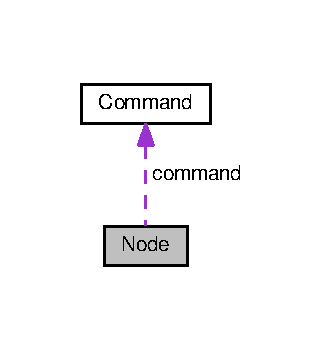
\includegraphics[width=156pt]{structNode__coll__graph}
\end{center}
\end{figure}
\subsection*{Public Member Functions}
\begin{DoxyCompactItemize}
\item 
\hyperlink{structNode_ad7a34779cad45d997bfd6d3d8043c75f}{Node} ()
\item 
\hyperlink{structNode_a277918b68827f6ffd8150f450b0c12c3}{Node} (const \hyperlink{structNode}{Node} \&n)
\item 
\hyperlink{structNode_a49671be091a3b75f20a4cdaf114dcdef}{Node} (\hyperlink{structNode}{Node} $\ast$n)
\item 
\hyperlink{structNode_aa0840c3cb5c7159be6d992adecd2097c}{$\sim$\-Node} ()
\item 
bool \hyperlink{structNode_a34785dbb41a8eed1a1871863300ab180}{operator==} (const \hyperlink{structNode}{Node} \&n) const 
\end{DoxyCompactItemize}
\subsection*{Public Attributes}
\begin{DoxyCompactItemize}
\item 
int \hyperlink{structNode_a59a543130a10c95f1e8642cf8c5645e8}{id}
\item 
\hyperlink{structCommand}{Command} \hyperlink{structNode_a77877b9758bdbfe6de9c1a9cafc76bd4}{command}
\item 
std\-::shared\-\_\-ptr$<$ \hyperlink{structNode}{Node} $>$ \hyperlink{structNode_ab452a3c22bdb42908e040e6f4fe4b097}{successor1}
\item 
std\-::shared\-\_\-ptr$<$ \hyperlink{structNode}{Node} $>$ \hyperlink{structNode_a1b5557700bd2ad4b58800bfa15999323}{successor2}
\end{DoxyCompactItemize}


\subsection{Detailed Description}
Represents a node in the \mbox{[}a\mbox{]}bstract \mbox{[}s\mbox{]}yntax \mbox{[}g\mbox{]}raph (A\-S\-G), each node also represents a command in the corresponding Rail programm. That means each node has a command to execute.

\begin{DoxyAuthor}{Author}
Christopher Zell \href{mailto:Zelldon91@googlemail.com}{\tt Zelldon91@googlemail.\-com}, Hanin Halawani 
\end{DoxyAuthor}


\subsection{Constructor \& Destructor Documentation}
\hypertarget{structNode_ad7a34779cad45d997bfd6d3d8043c75f}{\index{Node@{Node}!Node@{Node}}
\index{Node@{Node}!Node@{Node}}
\subsubsection[{Node}]{\setlength{\rightskip}{0pt plus 5cm}Node\-::\-Node (
\begin{DoxyParamCaption}
{}
\end{DoxyParamCaption}
)\hspace{0.3cm}{\ttfamily [inline]}}}\label{structNode_ad7a34779cad45d997bfd6d3d8043c75f}
The default ctor of the node, initialize the id of the node with 0. \hypertarget{structNode_a277918b68827f6ffd8150f450b0c12c3}{\index{Node@{Node}!Node@{Node}}
\index{Node@{Node}!Node@{Node}}
\subsubsection[{Node}]{\setlength{\rightskip}{0pt plus 5cm}Node\-::\-Node (
\begin{DoxyParamCaption}
\item[{const {\bf Node} \&}]{n}
\end{DoxyParamCaption}
)\hspace{0.3cm}{\ttfamily [inline]}}}\label{structNode_a277918b68827f6ffd8150f450b0c12c3}
The copy ctor of the node, copies the values of another node in the corresponding node. 
\begin{DoxyParams}{Parameters}
{\em n} & the node which will be copied \\
\hline
\end{DoxyParams}
\hypertarget{structNode_a49671be091a3b75f20a4cdaf114dcdef}{\index{Node@{Node}!Node@{Node}}
\index{Node@{Node}!Node@{Node}}
\subsubsection[{Node}]{\setlength{\rightskip}{0pt plus 5cm}Node\-::\-Node (
\begin{DoxyParamCaption}
\item[{{\bf Node} $\ast$}]{n}
\end{DoxyParamCaption}
)\hspace{0.3cm}{\ttfamily [inline]}}}\label{structNode_a49671be091a3b75f20a4cdaf114dcdef}
The copy ctor of the node, copies the values of another node in the corresponding node. 
\begin{DoxyParams}{Parameters}
{\em n} & the node which will be copied \\
\hline
\end{DoxyParams}
\hypertarget{structNode_aa0840c3cb5c7159be6d992adecd2097c}{\index{Node@{Node}!$\sim$\-Node@{$\sim$\-Node}}
\index{$\sim$\-Node@{$\sim$\-Node}!Node@{Node}}
\subsubsection[{$\sim$\-Node}]{\setlength{\rightskip}{0pt plus 5cm}Node\-::$\sim$\-Node (
\begin{DoxyParamCaption}
{}
\end{DoxyParamCaption}
)\hspace{0.3cm}{\ttfamily [inline]}}}\label{structNode_aa0840c3cb5c7159be6d992adecd2097c}
The destructor of the node, resets all existing smart pointers inside the node. 

\subsection{Member Function Documentation}
\hypertarget{structNode_a34785dbb41a8eed1a1871863300ab180}{\index{Node@{Node}!operator==@{operator==}}
\index{operator==@{operator==}!Node@{Node}}
\subsubsection[{operator==}]{\setlength{\rightskip}{0pt plus 5cm}bool Node\-::operator== (
\begin{DoxyParamCaption}
\item[{const {\bf Node} \&}]{n}
\end{DoxyParamCaption}
) const\hspace{0.3cm}{\ttfamily [inline]}}}\label{structNode_a34785dbb41a8eed1a1871863300ab180}
The equals operator which copares the id of the current with another node. If the ids are equal it returns true, otherwise false. 
\begin{DoxyParams}{Parameters}
{\em n} & the node which will be used for the comparison \\
\hline
\end{DoxyParams}
\begin{DoxyReturn}{Returns}
true if the ids are equal, false otherwise 
\end{DoxyReturn}


\subsection{Member Data Documentation}
\hypertarget{structNode_a77877b9758bdbfe6de9c1a9cafc76bd4}{\index{Node@{Node}!command@{command}}
\index{command@{command}!Node@{Node}}
\subsubsection[{command}]{\setlength{\rightskip}{0pt plus 5cm}{\bf Command} Node\-::command}}\label{structNode_a77877b9758bdbfe6de9c1a9cafc76bd4}
The corresponding command of the node. \hypertarget{structNode_a59a543130a10c95f1e8642cf8c5645e8}{\index{Node@{Node}!id@{id}}
\index{id@{id}!Node@{Node}}
\subsubsection[{id}]{\setlength{\rightskip}{0pt plus 5cm}int Node\-::id}}\label{structNode_a59a543130a10c95f1e8642cf8c5645e8}
The I\-D of the node, which identifies the node. \hypertarget{structNode_ab452a3c22bdb42908e040e6f4fe4b097}{\index{Node@{Node}!successor1@{successor1}}
\index{successor1@{successor1}!Node@{Node}}
\subsubsection[{successor1}]{\setlength{\rightskip}{0pt plus 5cm}std\-::shared\-\_\-ptr$<${\bf Node}$>$ Node\-::successor1}}\label{structNode_ab452a3c22bdb42908e040e6f4fe4b097}
The first successor of the current node. {\bfseries This successor is always the true path and is set if a successor exists.} That means if the node (command) is not \#, what means end, a successor must exists and these is placed in the successor1. \hypertarget{structNode_a1b5557700bd2ad4b58800bfa15999323}{\index{Node@{Node}!successor2@{successor2}}
\index{successor2@{successor2}!Node@{Node}}
\subsubsection[{successor2}]{\setlength{\rightskip}{0pt plus 5cm}std\-::shared\-\_\-ptr$<${\bf Node}$>$ Node\-::successor2}}\label{structNode_a1b5557700bd2ad4b58800bfa15999323}
The second successor of the current node. This successor is only not null if the current node is a junction, like $<$, $>$, V or $^\wedge$. {\bfseries The successor2 contains the false path of the junction.} 

The documentation for this struct was generated from the following file\-:\begin{DoxyCompactItemize}
\item 
common/ast/\hyperlink{ast_8h}{ast.\-h}\end{DoxyCompactItemize}

\hypertarget{structoffsetvalues}{\section{offsetvalues Struct Reference}
\label{structoffsetvalues}\index{offsetvalues@{offsetvalues}}
}


{\ttfamily \#include $<$Parser.\-h$>$}

\subsection*{Public Attributes}
\begin{DoxyCompactItemize}
\item 
int \hyperlink{structoffsetvalues_ad39c312efc78e0df6c9b11c24f3b41a7}{offsets} \mbox{[}3\mbox{]}
\end{DoxyCompactItemize}


\subsection{Member Data Documentation}
\hypertarget{structoffsetvalues_ad39c312efc78e0df6c9b11c24f3b41a7}{\index{offsetvalues@{offsetvalues}!offsets@{offsets}}
\index{offsets@{offsets}!offsetvalues@{offsetvalues}}
\subsubsection[{offsets}]{\setlength{\rightskip}{0pt plus 5cm}int offsetvalues\-::offsets\mbox{[}3\mbox{]}}}\label{structoffsetvalues_ad39c312efc78e0df6c9b11c24f3b41a7}


The documentation for this struct was generated from the following file\-:\begin{DoxyCompactItemize}
\item 
frontend/\hyperlink{Parser_8h}{Parser.\-h}\end{DoxyCompactItemize}

\hypertarget{classParse__Exception}{\section{Parse\-\_\-\-Exception Class Reference}
\label{classParse__Exception}\index{Parse\-\_\-\-Exception@{Parse\-\_\-\-Exception}}
}


{\ttfamily \#include $<$Parse\-\_\-\-Exception.\-h$>$}



Inheritance diagram for Parse\-\_\-\-Exception\-:
\nopagebreak
\begin{figure}[H]
\begin{center}
\leavevmode
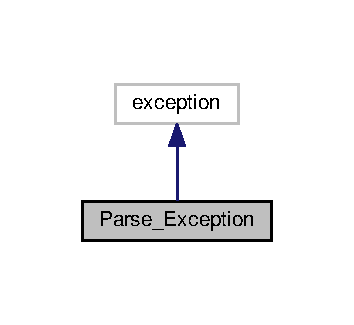
\includegraphics[width=170pt]{classParse__Exception__inherit__graph}
\end{center}
\end{figure}


Collaboration diagram for Parse\-\_\-\-Exception\-:
\nopagebreak
\begin{figure}[H]
\begin{center}
\leavevmode
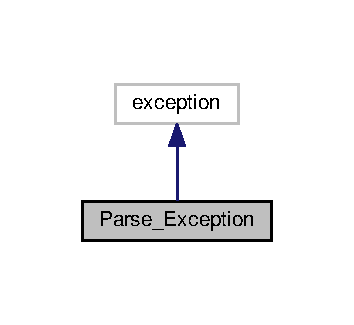
\includegraphics[width=170pt]{classParse__Exception__coll__graph}
\end{center}
\end{figure}
\subsection*{Public Member Functions}
\begin{DoxyCompactItemize}
\item 
void \hyperlink{classParse__Exception_a4a100fe9ff60bbc3a90413d46d88a5fa}{set\-\_\-msg} (const std\-::string \&m)
\end{DoxyCompactItemize}


\subsection{Member Function Documentation}
\hypertarget{classParse__Exception_a4a100fe9ff60bbc3a90413d46d88a5fa}{\index{Parse\-\_\-\-Exception@{Parse\-\_\-\-Exception}!set\-\_\-msg@{set\-\_\-msg}}
\index{set\-\_\-msg@{set\-\_\-msg}!Parse_Exception@{Parse\-\_\-\-Exception}}
\subsubsection[{set\-\_\-msg}]{\setlength{\rightskip}{0pt plus 5cm}void Parse\-\_\-\-Exception\-::set\-\_\-msg (
\begin{DoxyParamCaption}
\item[{const std\-::string \&}]{m}
\end{DoxyParamCaption}
)\hspace{0.3cm}{\ttfamily [inline]}}}\label{classParse__Exception_a4a100fe9ff60bbc3a90413d46d88a5fa}


The documentation for this class was generated from the following file\-:\begin{DoxyCompactItemize}
\item 
frontend/\hyperlink{Parse__Exception_8h}{Parse\-\_\-\-Exception.\-h}\end{DoxyCompactItemize}

\hypertarget{classParser}{\section{Parser Class Reference}
\label{classParser}\index{Parser@{Parser}}
}


{\ttfamily \#include $<$Parser.\-h$>$}

\subsection*{Public Member Functions}
\begin{DoxyCompactItemize}
\item 
\hyperlink{classParser_ad9f465482450083d7037f6954a352d7b}{Parser} (\hyperlink{structBoardContainer}{Board\-Container}, string)
\item 
shared\-\_\-ptr$<$ \hyperlink{classAdjacency__list}{Adjacency\-\_\-list} $>$ \hyperlink{classParser_a7d04bed7e3f12b585ebe138e785cb3c0}{parse\-Graph} ()
\end{DoxyCompactItemize}
\subsection*{Public Attributes}
\begin{DoxyCompactItemize}
\item 
string \hyperlink{classParser_aba956cc0f04b554441a05fd595634d80}{error\-Message}
\end{DoxyCompactItemize}


\subsection{Constructor \& Destructor Documentation}
\hypertarget{classParser_ad9f465482450083d7037f6954a352d7b}{\index{Parser@{Parser}!Parser@{Parser}}
\index{Parser@{Parser}!Parser@{Parser}}
\subsubsection[{Parser}]{\setlength{\rightskip}{0pt plus 5cm}Parser\-::\-Parser (
\begin{DoxyParamCaption}
\item[{{\bf Board\-Container}}]{board\-Container, }
\item[{string}]{graph\-Name}
\end{DoxyParamCaption}
)}}\label{classParser_ad9f465482450083d7037f6954a352d7b}


\subsection{Member Function Documentation}
\hypertarget{classParser_a7d04bed7e3f12b585ebe138e785cb3c0}{\index{Parser@{Parser}!parse\-Graph@{parse\-Graph}}
\index{parse\-Graph@{parse\-Graph}!Parser@{Parser}}
\subsubsection[{parse\-Graph}]{\setlength{\rightskip}{0pt plus 5cm}shared\-\_\-ptr$<$ {\bf Adjacency\-\_\-list} $>$ Parser\-::parse\-Graph (
\begin{DoxyParamCaption}
{}
\end{DoxyParamCaption}
)}}\label{classParser_a7d04bed7e3f12b585ebe138e785cb3c0}


\subsection{Member Data Documentation}
\hypertarget{classParser_aba956cc0f04b554441a05fd595634d80}{\index{Parser@{Parser}!error\-Message@{error\-Message}}
\index{error\-Message@{error\-Message}!Parser@{Parser}}
\subsubsection[{error\-Message}]{\setlength{\rightskip}{0pt plus 5cm}string Parser\-::error\-Message}}\label{classParser_aba956cc0f04b554441a05fd595634d80}


The documentation for this class was generated from the following files\-:\begin{DoxyCompactItemize}
\item 
frontend/\hyperlink{Parser_8h}{Parser.\-h}\item 
frontend/\hyperlink{Parser_8cpp}{Parser.\-cpp}\end{DoxyCompactItemize}

\hypertarget{classRailFunction}{\section{Rail\-Function Class Reference}
\label{classRailFunction}\index{Rail\-Function@{Rail\-Function}}
}


{\ttfamily \#include $<$lexer.\-h$>$}

\subsection*{Public Member Functions}
\begin{DoxyCompactItemize}
\item 
string \hyperlink{classRailFunction_a001ae48860debf0509bbf761f089092f}{get\-Name} ()
\item 
void \hyperlink{classRailFunction_aeca8e805b9c06d51db9300f6c69009b8}{set\-Name} (string name)
\item 
void \hyperlink{classRailFunction_a485bc940067a84e6e3e9edcae021ab34}{init\-Data} ()
\item 
char \hyperlink{classRailFunction_aa732e25133a0fe107af1ec760e131279}{get\-Data} (int offset\-X, int offset\-Y)
\item 
void \hyperlink{classRailFunction_aa1ba9b04faf9ac135409271c0d39b085}{set\-Data} (int offset\-X, int offset\-Y, char c)
\item 
void \hyperlink{classRailFunction_a7779d0455d34397801d8d5b6891cf6fb}{print\-Rails} ()
\item 
void \hyperlink{classRailFunction_aa81a3bbfb960bbf7bebb5f342519805e}{lex} (const string \&filename)
\end{DoxyCompactItemize}
\subsection*{Public Attributes}
\begin{DoxyCompactItemize}
\item 
char \hyperlink{classRailFunction_a7d88f1aa53e86f9e76d60476265bed39}{code} \mbox{[}\hyperlink{lexer_8h_a3b95e0254661c995b723a9b150a821c1}{M\-A\-X\-\_\-\-C\-H\-A\-R\-S\-\_\-\-P\-E\-R\-\_\-\-L\-I\-N\-E}\mbox{]}\mbox{[}\hyperlink{lexer_8h_afe8deb2b6b8318fa96d532e836f97a20}{M\-A\-X\-\_\-\-L\-I\-N\-E\-S\-\_\-\-P\-E\-R\-\_\-\-F\-U\-N\-C\-T\-I\-O\-N}\mbox{]}
\end{DoxyCompactItemize}


\subsection{Member Function Documentation}
\hypertarget{classRailFunction_aa732e25133a0fe107af1ec760e131279}{\index{Rail\-Function@{Rail\-Function}!get\-Data@{get\-Data}}
\index{get\-Data@{get\-Data}!RailFunction@{Rail\-Function}}
\subsubsection[{get\-Data}]{\setlength{\rightskip}{0pt plus 5cm}char Rail\-Function\-::get\-Data (
\begin{DoxyParamCaption}
\item[{int}]{offset\-X, }
\item[{int}]{offset\-Y}
\end{DoxyParamCaption}
)}}\label{classRailFunction_aa732e25133a0fe107af1ec760e131279}
\hypertarget{classRailFunction_a001ae48860debf0509bbf761f089092f}{\index{Rail\-Function@{Rail\-Function}!get\-Name@{get\-Name}}
\index{get\-Name@{get\-Name}!RailFunction@{Rail\-Function}}
\subsubsection[{get\-Name}]{\setlength{\rightskip}{0pt plus 5cm}string Rail\-Function\-::get\-Name (
\begin{DoxyParamCaption}
{}
\end{DoxyParamCaption}
)}}\label{classRailFunction_a001ae48860debf0509bbf761f089092f}
\hypertarget{classRailFunction_a485bc940067a84e6e3e9edcae021ab34}{\index{Rail\-Function@{Rail\-Function}!init\-Data@{init\-Data}}
\index{init\-Data@{init\-Data}!RailFunction@{Rail\-Function}}
\subsubsection[{init\-Data}]{\setlength{\rightskip}{0pt plus 5cm}void Rail\-Function\-::init\-Data (
\begin{DoxyParamCaption}
{}
\end{DoxyParamCaption}
)}}\label{classRailFunction_a485bc940067a84e6e3e9edcae021ab34}


Here is the call graph for this function\-:
\nopagebreak
\begin{figure}[H]
\begin{center}
\leavevmode
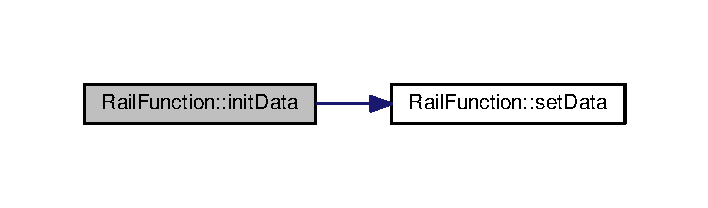
\includegraphics[width=340pt]{classRailFunction_a485bc940067a84e6e3e9edcae021ab34_cgraph}
\end{center}
\end{figure}


\hypertarget{classRailFunction_aa81a3bbfb960bbf7bebb5f342519805e}{\index{Rail\-Function@{Rail\-Function}!lex@{lex}}
\index{lex@{lex}!RailFunction@{Rail\-Function}}
\subsubsection[{lex}]{\setlength{\rightskip}{0pt plus 5cm}void Rail\-Function\-::lex (
\begin{DoxyParamCaption}
\item[{const string \&}]{filename}
\end{DoxyParamCaption}
)}}\label{classRailFunction_aa81a3bbfb960bbf7bebb5f342519805e}
\hypertarget{classRailFunction_a7779d0455d34397801d8d5b6891cf6fb}{\index{Rail\-Function@{Rail\-Function}!print\-Rails@{print\-Rails}}
\index{print\-Rails@{print\-Rails}!RailFunction@{Rail\-Function}}
\subsubsection[{print\-Rails}]{\setlength{\rightskip}{0pt plus 5cm}void Rail\-Function\-::print\-Rails (
\begin{DoxyParamCaption}
{}
\end{DoxyParamCaption}
)}}\label{classRailFunction_a7779d0455d34397801d8d5b6891cf6fb}


Here is the call graph for this function\-:
\nopagebreak
\begin{figure}[H]
\begin{center}
\leavevmode
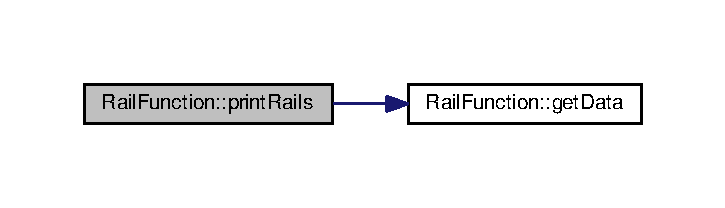
\includegraphics[width=348pt]{classRailFunction_a7779d0455d34397801d8d5b6891cf6fb_cgraph}
\end{center}
\end{figure}


\hypertarget{classRailFunction_aa1ba9b04faf9ac135409271c0d39b085}{\index{Rail\-Function@{Rail\-Function}!set\-Data@{set\-Data}}
\index{set\-Data@{set\-Data}!RailFunction@{Rail\-Function}}
\subsubsection[{set\-Data}]{\setlength{\rightskip}{0pt plus 5cm}void Rail\-Function\-::set\-Data (
\begin{DoxyParamCaption}
\item[{int}]{offset\-X, }
\item[{int}]{offset\-Y, }
\item[{char}]{c}
\end{DoxyParamCaption}
)}}\label{classRailFunction_aa1ba9b04faf9ac135409271c0d39b085}
\hypertarget{classRailFunction_aeca8e805b9c06d51db9300f6c69009b8}{\index{Rail\-Function@{Rail\-Function}!set\-Name@{set\-Name}}
\index{set\-Name@{set\-Name}!RailFunction@{Rail\-Function}}
\subsubsection[{set\-Name}]{\setlength{\rightskip}{0pt plus 5cm}void Rail\-Function\-::set\-Name (
\begin{DoxyParamCaption}
\item[{string}]{name}
\end{DoxyParamCaption}
)}}\label{classRailFunction_aeca8e805b9c06d51db9300f6c69009b8}


\subsection{Member Data Documentation}
\hypertarget{classRailFunction_a7d88f1aa53e86f9e76d60476265bed39}{\index{Rail\-Function@{Rail\-Function}!code@{code}}
\index{code@{code}!RailFunction@{Rail\-Function}}
\subsubsection[{code}]{\setlength{\rightskip}{0pt plus 5cm}char Rail\-Function\-::code\mbox{[}{\bf M\-A\-X\-\_\-\-C\-H\-A\-R\-S\-\_\-\-P\-E\-R\-\_\-\-L\-I\-N\-E}\mbox{]}\mbox{[}{\bf M\-A\-X\-\_\-\-L\-I\-N\-E\-S\-\_\-\-P\-E\-R\-\_\-\-F\-U\-N\-C\-T\-I\-O\-N}\mbox{]}}}\label{classRailFunction_a7d88f1aa53e86f9e76d60476265bed39}


The documentation for this class was generated from the following files\-:\begin{DoxyCompactItemize}
\item 
frontend/parse/\hyperlink{lexer_8h}{lexer.\-h}\item 
frontend/parse/\hyperlink{lexer_8cpp}{lexer.\-cpp}\end{DoxyCompactItemize}

\chapter{File Documentation}
\hypertarget{backend_8cc}{\section{backend/backend.cc File Reference}
\label{backend_8cc}\index{backend/backend.\-cc@{backend/backend.\-cc}}
}
{\ttfamily \#include \char`\"{}backend/backend.\-h\char`\"{}}\\*
{\ttfamily \#include \char`\"{}backend/classfile/classfile\-\_\-writer.\-h\char`\"{}}\\*
{\ttfamily \#include \char`\"{}backend/codegen/bytecode\-\_\-generator.\-h\char`\"{}}\\*
{\ttfamily \#include \char`\"{}frontend/\-Graphs.\-h\char`\"{}}\\*
Include dependency graph for backend.\-cc\-:
\nopagebreak
\begin{figure}[H]
\begin{center}
\leavevmode
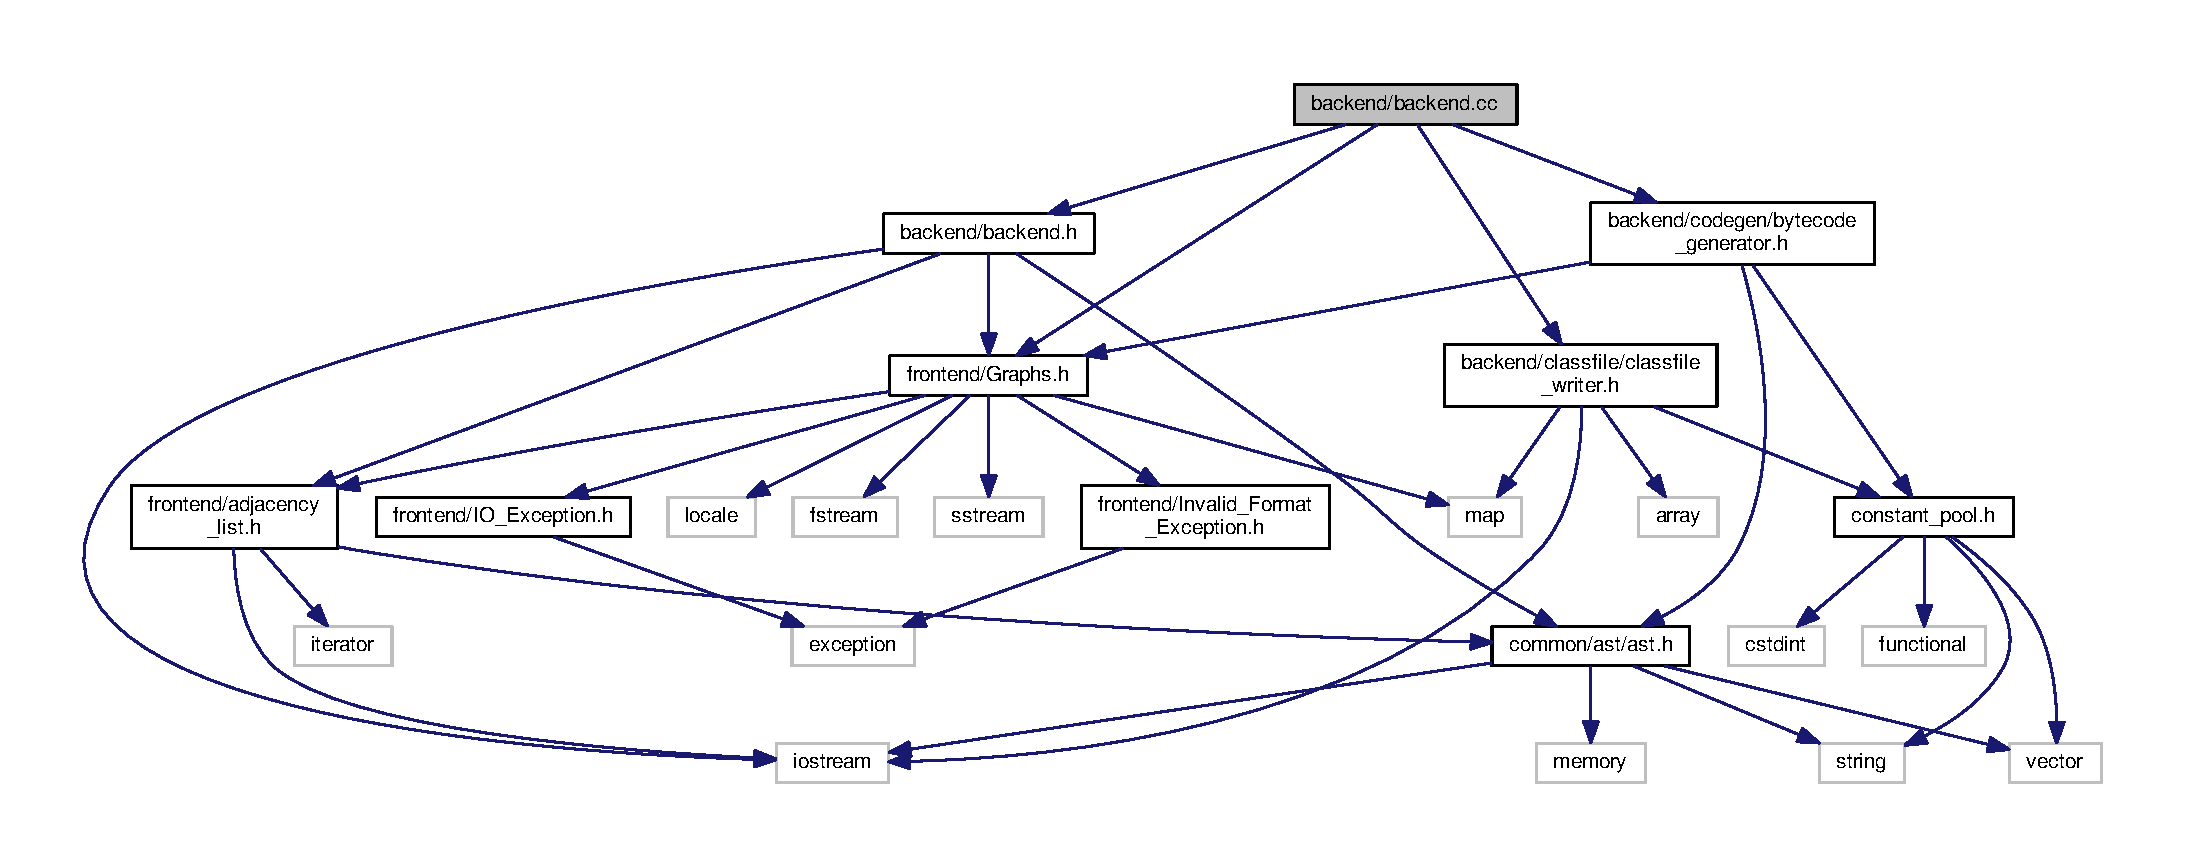
\includegraphics[width=350pt]{backend_8cc__incl}
\end{center}
\end{figure}

\hypertarget{backend_8h}{\section{backend/backend.h File Reference}
\label{backend_8h}\index{backend/backend.\-h@{backend/backend.\-h}}
}
{\ttfamily \#include $<$iostream$>$}\\*
{\ttfamily \#include $<$common/ast/ast.\-h$>$}\\*
{\ttfamily \#include $<$frontend/adjacency\-\_\-list.\-h$>$}\\*
{\ttfamily \#include $<$frontend/\-Graphs.\-h$>$}\\*
Include dependency graph for backend.\-h\-:
\nopagebreak
\begin{figure}[H]
\begin{center}
\leavevmode
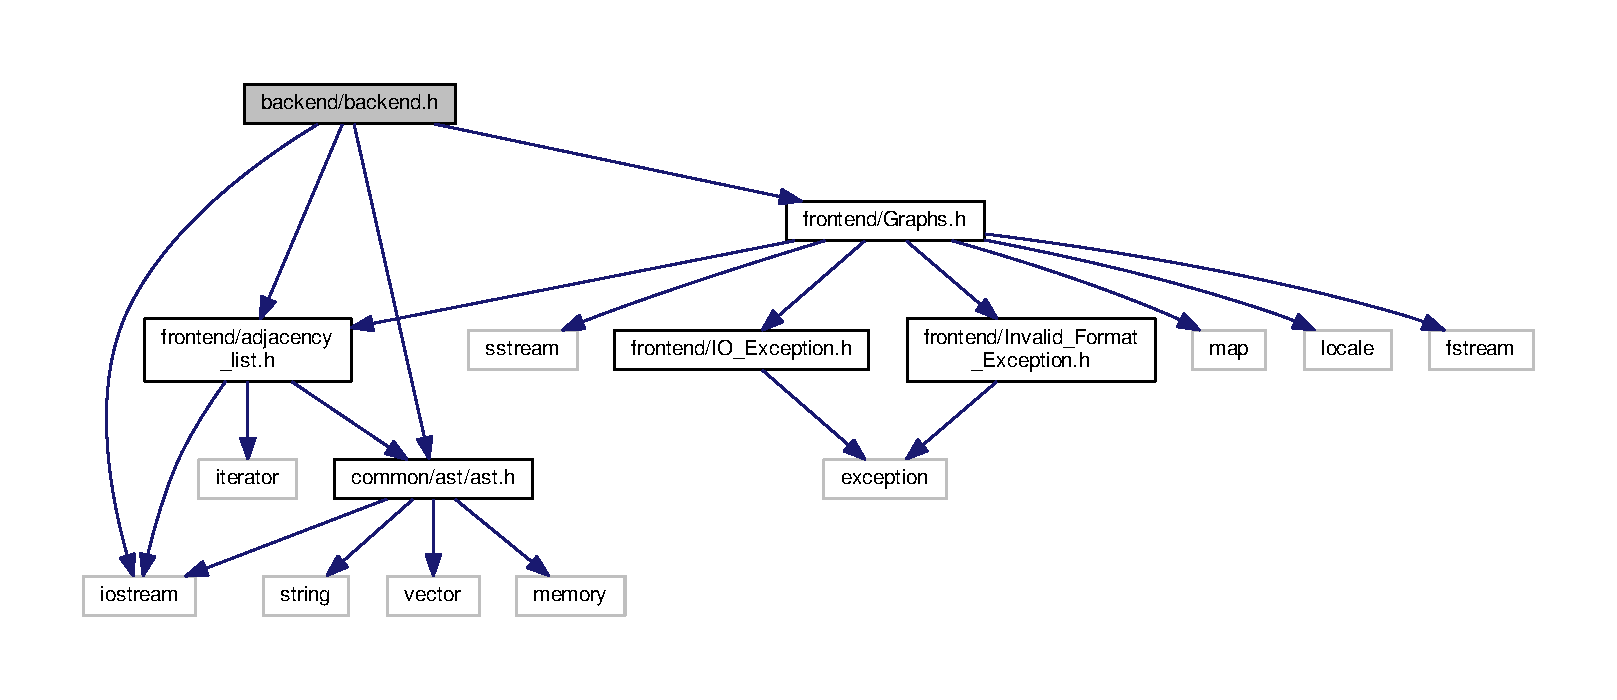
\includegraphics[width=350pt]{backend_8h__incl}
\end{center}
\end{figure}
This graph shows which files directly or indirectly include this file\-:
\nopagebreak
\begin{figure}[H]
\begin{center}
\leavevmode
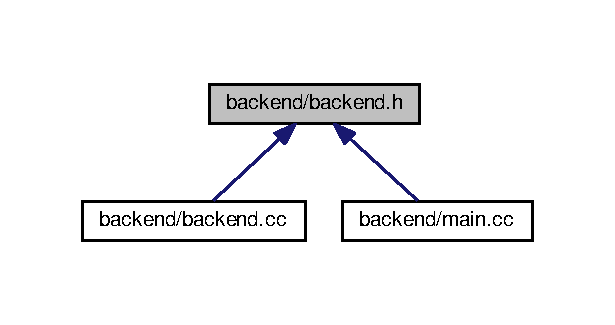
\includegraphics[width=295pt]{backend_8h__dep__incl}
\end{center}
\end{figure}
\subsection*{Classes}
\begin{DoxyCompactItemize}
\item 
class \hyperlink{classBackend}{Backend}
\end{DoxyCompactItemize}

\hypertarget{classfile__writer_8cc}{\section{backend/classfile/classfile\-\_\-writer.cc File Reference}
\label{classfile__writer_8cc}\index{backend/classfile/classfile\-\_\-writer.\-cc@{backend/classfile/classfile\-\_\-writer.\-cc}}
}
{\ttfamily \#include $<$backend/classfile/classfile\-\_\-writer.\-h$>$}\\*
{\ttfamily \#include $<$backend/classfile/constant\-\_\-pool.\-h$>$}\\*
{\ttfamily \#include $<$array$>$}\\*
{\ttfamily \#include $<$iostream$>$}\\*
{\ttfamily \#include $<$map$>$}\\*
{\ttfamily \#include $<$string$>$}\\*
Include dependency graph for classfile\-\_\-writer.\-cc\-:
\nopagebreak
\begin{figure}[H]
\begin{center}
\leavevmode
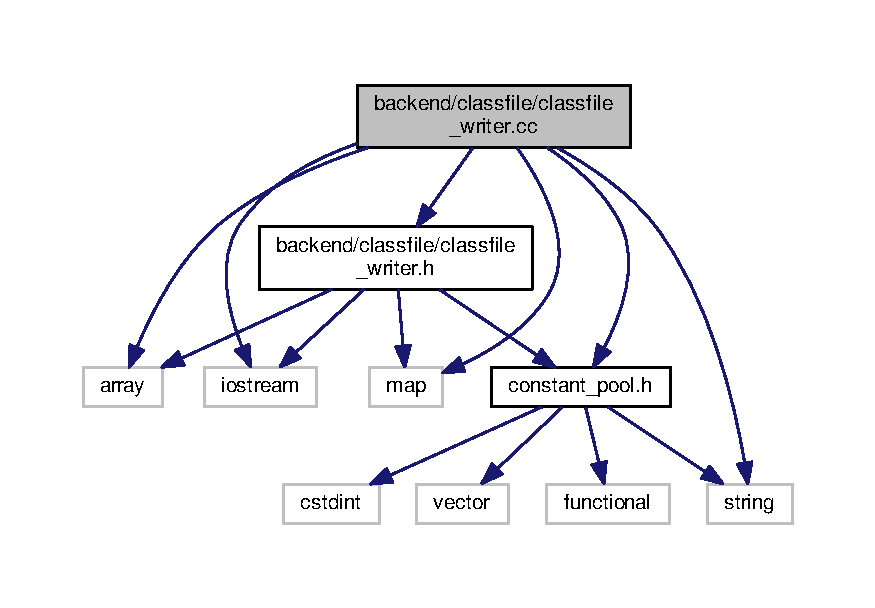
\includegraphics[width=350pt]{classfile__writer_8cc__incl}
\end{center}
\end{figure}

\hypertarget{classfile__writer_8h}{\section{backend/classfile/classfile\-\_\-writer.h File Reference}
\label{classfile__writer_8h}\index{backend/classfile/classfile\-\_\-writer.\-h@{backend/classfile/classfile\-\_\-writer.\-h}}
}
{\ttfamily \#include $<$array$>$}\\*
{\ttfamily \#include $<$iostream$>$}\\*
{\ttfamily \#include $<$map$>$}\\*
{\ttfamily \#include \char`\"{}constant\-\_\-pool.\-h\char`\"{}}\\*
Include dependency graph for classfile\-\_\-writer.\-h\-:
\nopagebreak
\begin{figure}[H]
\begin{center}
\leavevmode
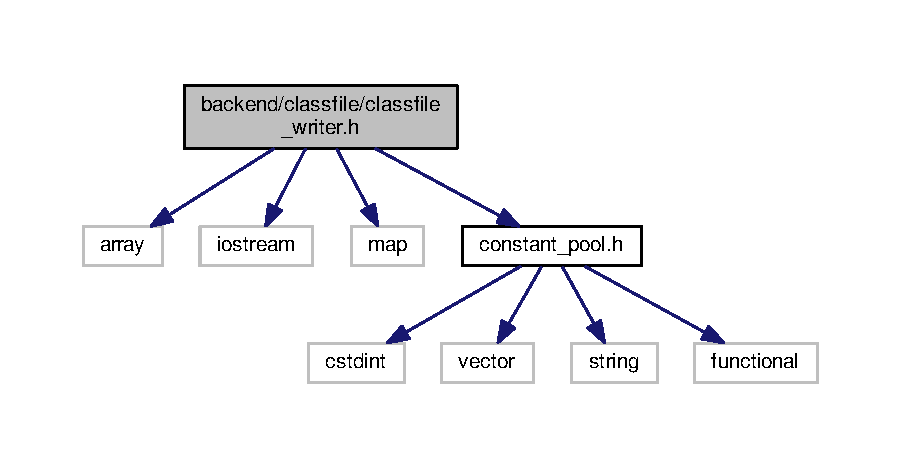
\includegraphics[width=350pt]{classfile__writer_8h__incl}
\end{center}
\end{figure}
This graph shows which files directly or indirectly include this file\-:
\nopagebreak
\begin{figure}[H]
\begin{center}
\leavevmode
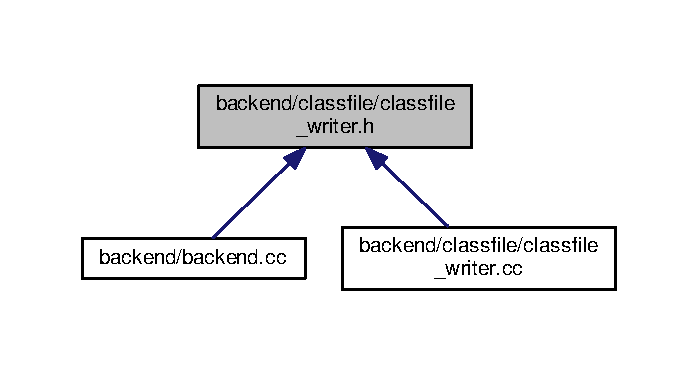
\includegraphics[width=335pt]{classfile__writer_8h__dep__incl}
\end{center}
\end{figure}
\subsection*{Classes}
\begin{DoxyCompactItemize}
\item 
class \hyperlink{classClassfileWriter}{Classfile\-Writer}
\end{DoxyCompactItemize}

\hypertarget{constant__pool_8cc}{\section{backend/classfile/constant\-\_\-pool.cc File Reference}
\label{constant__pool_8cc}\index{backend/classfile/constant\-\_\-pool.\-cc@{backend/classfile/constant\-\_\-pool.\-cc}}
}
{\ttfamily \#include $<$backend/classfile/constant\-\_\-pool.\-h$>$}\\*
{\ttfamily \#include $<$algorithm$>$}\\*
Include dependency graph for constant\-\_\-pool.\-cc\-:
\nopagebreak
\begin{figure}[H]
\begin{center}
\leavevmode
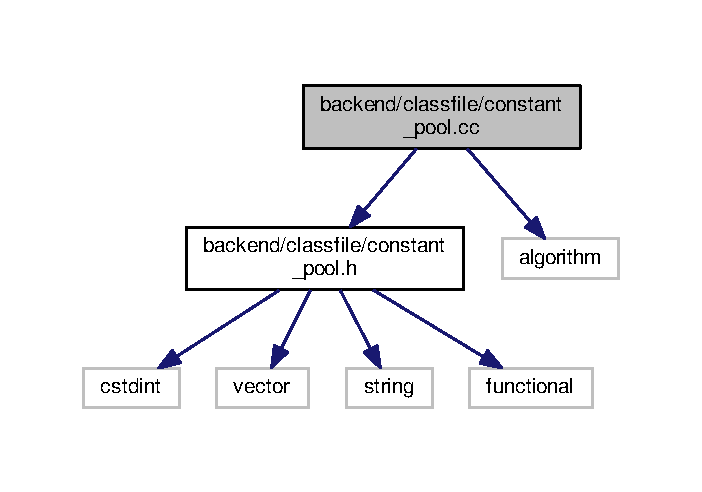
\includegraphics[width=337pt]{constant__pool_8cc__incl}
\end{center}
\end{figure}

\hypertarget{constant__pool_8h}{\section{backend/classfile/constant\-\_\-pool.h File Reference}
\label{constant__pool_8h}\index{backend/classfile/constant\-\_\-pool.\-h@{backend/classfile/constant\-\_\-pool.\-h}}
}
{\ttfamily \#include $<$cstdint$>$}\\*
{\ttfamily \#include $<$vector$>$}\\*
{\ttfamily \#include $<$string$>$}\\*
{\ttfamily \#include $<$functional$>$}\\*
Include dependency graph for constant\-\_\-pool.\-h\-:
\nopagebreak
\begin{figure}[H]
\begin{center}
\leavevmode
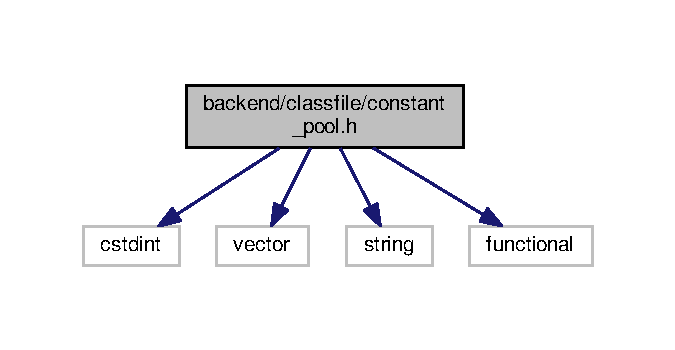
\includegraphics[width=324pt]{constant__pool_8h__incl}
\end{center}
\end{figure}
This graph shows which files directly or indirectly include this file\-:
\nopagebreak
\begin{figure}[H]
\begin{center}
\leavevmode
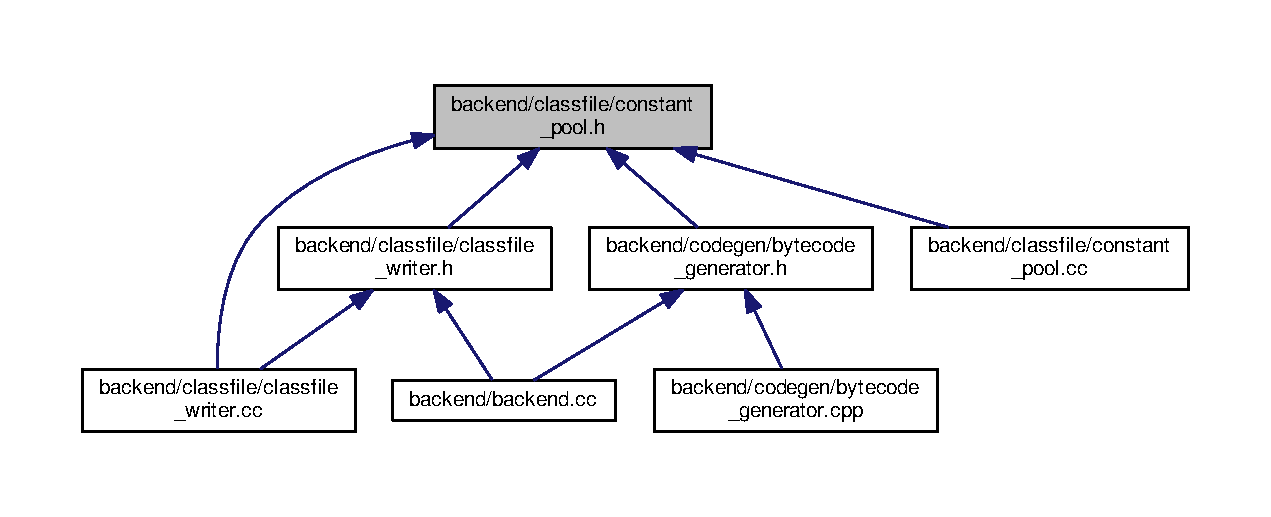
\includegraphics[width=350pt]{constant__pool_8h__dep__incl}
\end{center}
\end{figure}
\subsection*{Classes}
\begin{DoxyCompactItemize}
\item 
class \hyperlink{classItem}{Item}
\item 
class \hyperlink{classConstantPool}{Constant\-Pool}
\end{DoxyCompactItemize}

\hypertarget{bytecode__generator_8cpp}{\section{backend/codegen/bytecode\-\_\-generator.cpp File Reference}
\label{bytecode__generator_8cpp}\index{backend/codegen/bytecode\-\_\-generator.\-cpp@{backend/codegen/bytecode\-\_\-generator.\-cpp}}
}
{\ttfamily \#include \char`\"{}backend/codegen/bytecode\-\_\-generator.\-h\char`\"{}}\\*
{\ttfamily \#include $<$cstdint$>$}\\*
Include dependency graph for bytecode\-\_\-generator.\-cpp\-:
\nopagebreak
\begin{figure}[H]
\begin{center}
\leavevmode
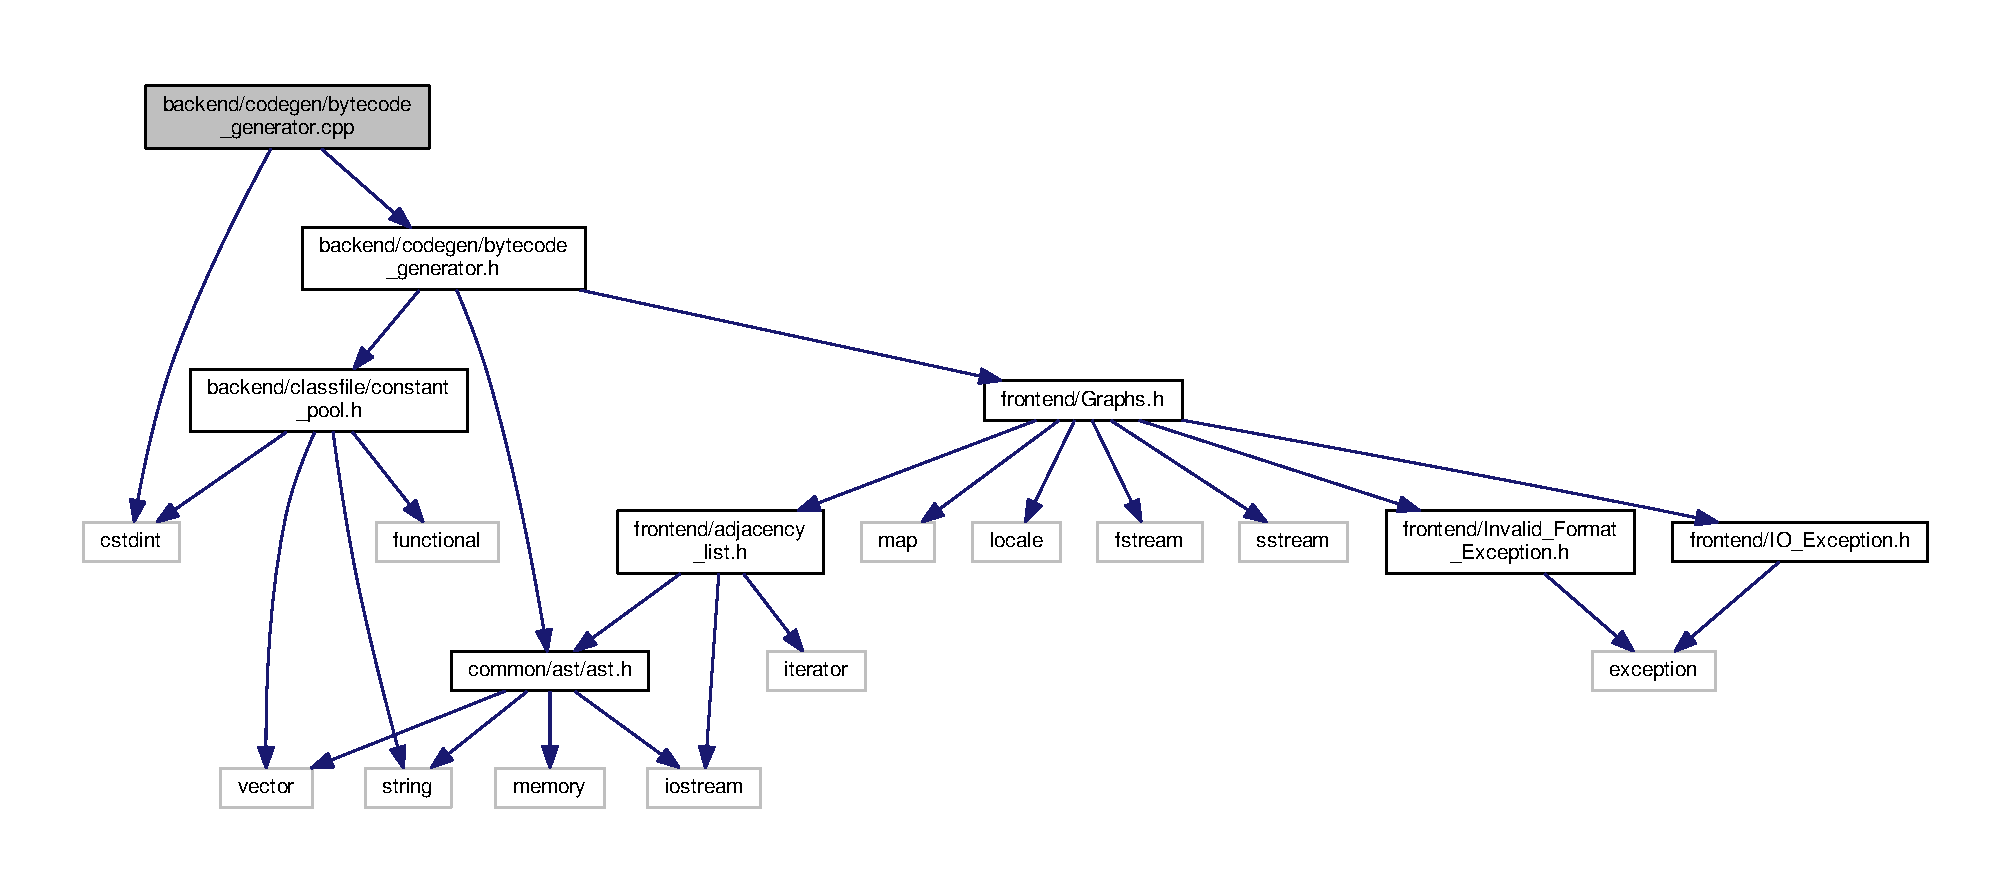
\includegraphics[width=350pt]{bytecode__generator_8cpp__incl}
\end{center}
\end{figure}

\hypertarget{bytecode__generator_8h}{\section{backend/codegen/bytecode\-\_\-generator.h File Reference}
\label{bytecode__generator_8h}\index{backend/codegen/bytecode\-\_\-generator.\-h@{backend/codegen/bytecode\-\_\-generator.\-h}}
}
{\ttfamily \#include \char`\"{}backend/classfile/constant\-\_\-pool.\-h\char`\"{}}\\*
{\ttfamily \#include \char`\"{}common/ast/ast.\-h\char`\"{}}\\*
{\ttfamily \#include \char`\"{}frontend/\-Graphs.\-h\char`\"{}}\\*
Include dependency graph for bytecode\-\_\-generator.\-h\-:
\nopagebreak
\begin{figure}[H]
\begin{center}
\leavevmode
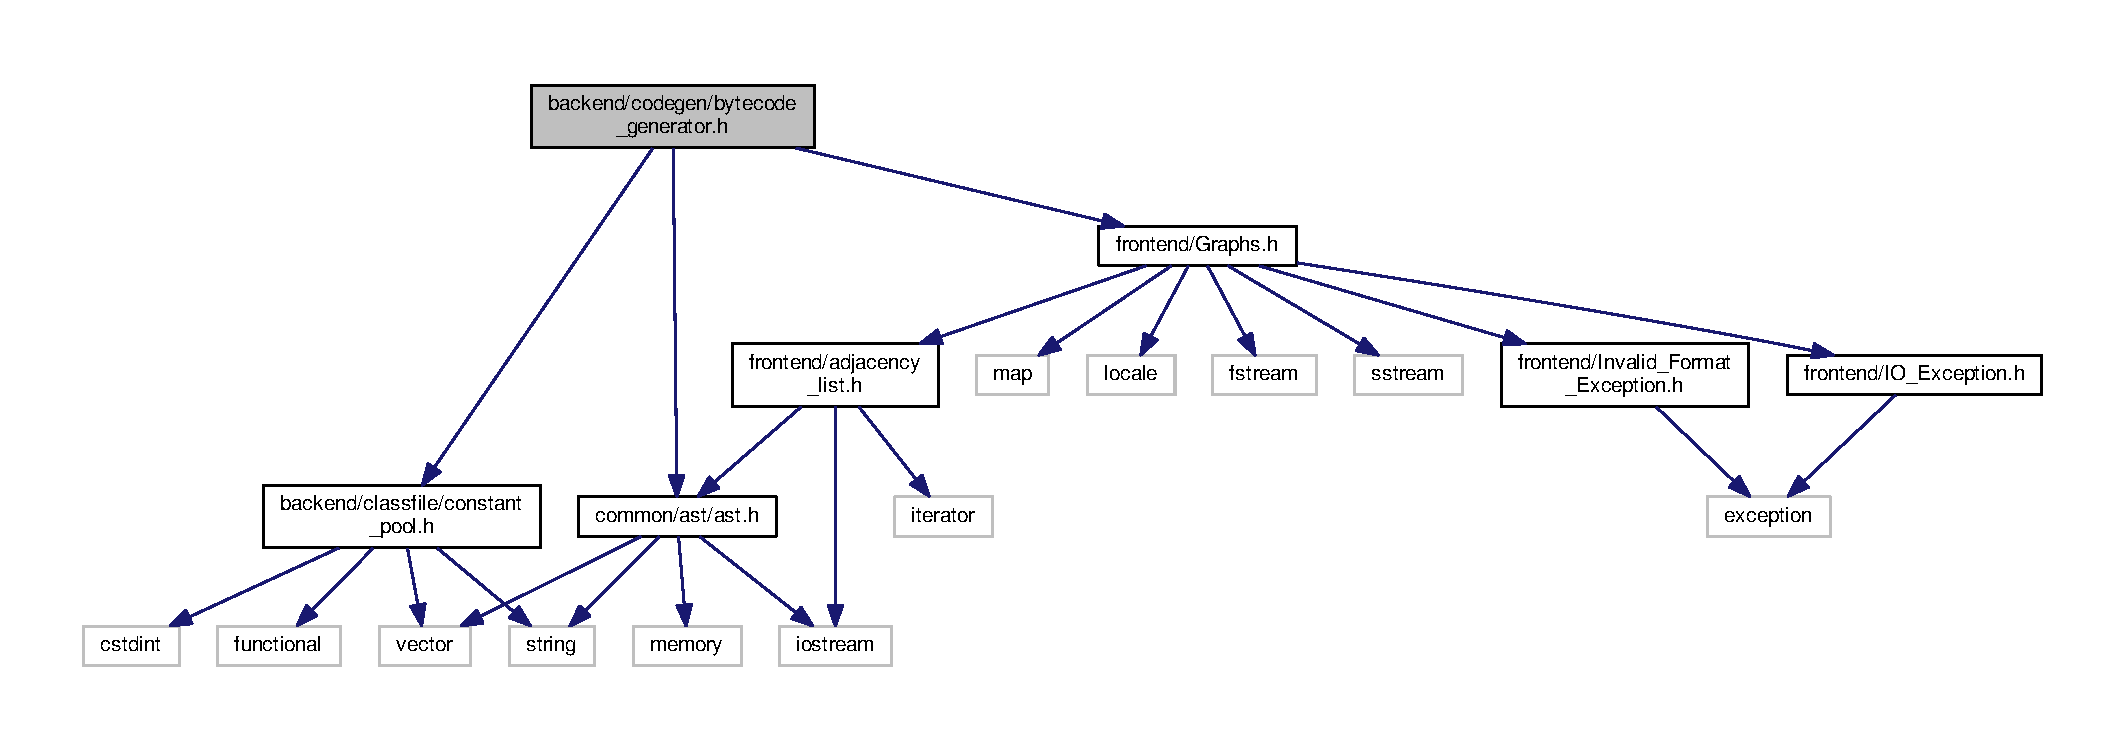
\includegraphics[width=350pt]{bytecode__generator_8h__incl}
\end{center}
\end{figure}
This graph shows which files directly or indirectly include this file\-:
\nopagebreak
\begin{figure}[H]
\begin{center}
\leavevmode
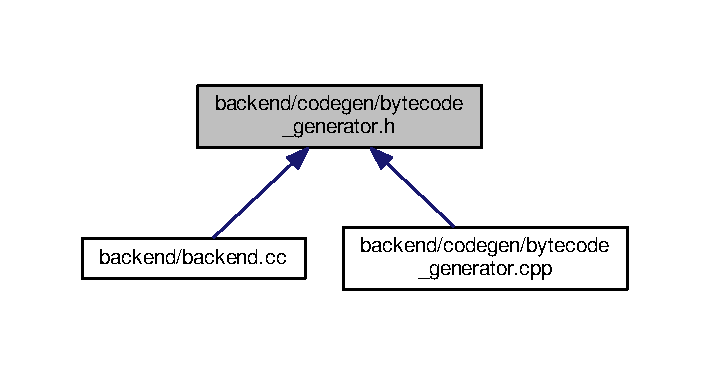
\includegraphics[width=341pt]{bytecode__generator_8h__dep__incl}
\end{center}
\end{figure}
\subsection*{Classes}
\begin{DoxyCompactItemize}
\item 
class \hyperlink{classBytecodeGenerator}{Bytecode\-Generator}
\end{DoxyCompactItemize}

\hypertarget{main_8cc}{\section{backend/main.cc File Reference}
\label{main_8cc}\index{backend/main.\-cc@{backend/main.\-cc}}
}
{\ttfamily \#include $<$fstream$>$}\\*
{\ttfamily \#include $<$iostream$>$}\\*
{\ttfamily \#include $<$backend/backend.\-h$>$}\\*
Include dependency graph for main.\-cc\-:
\nopagebreak
\begin{figure}[H]
\begin{center}
\leavevmode
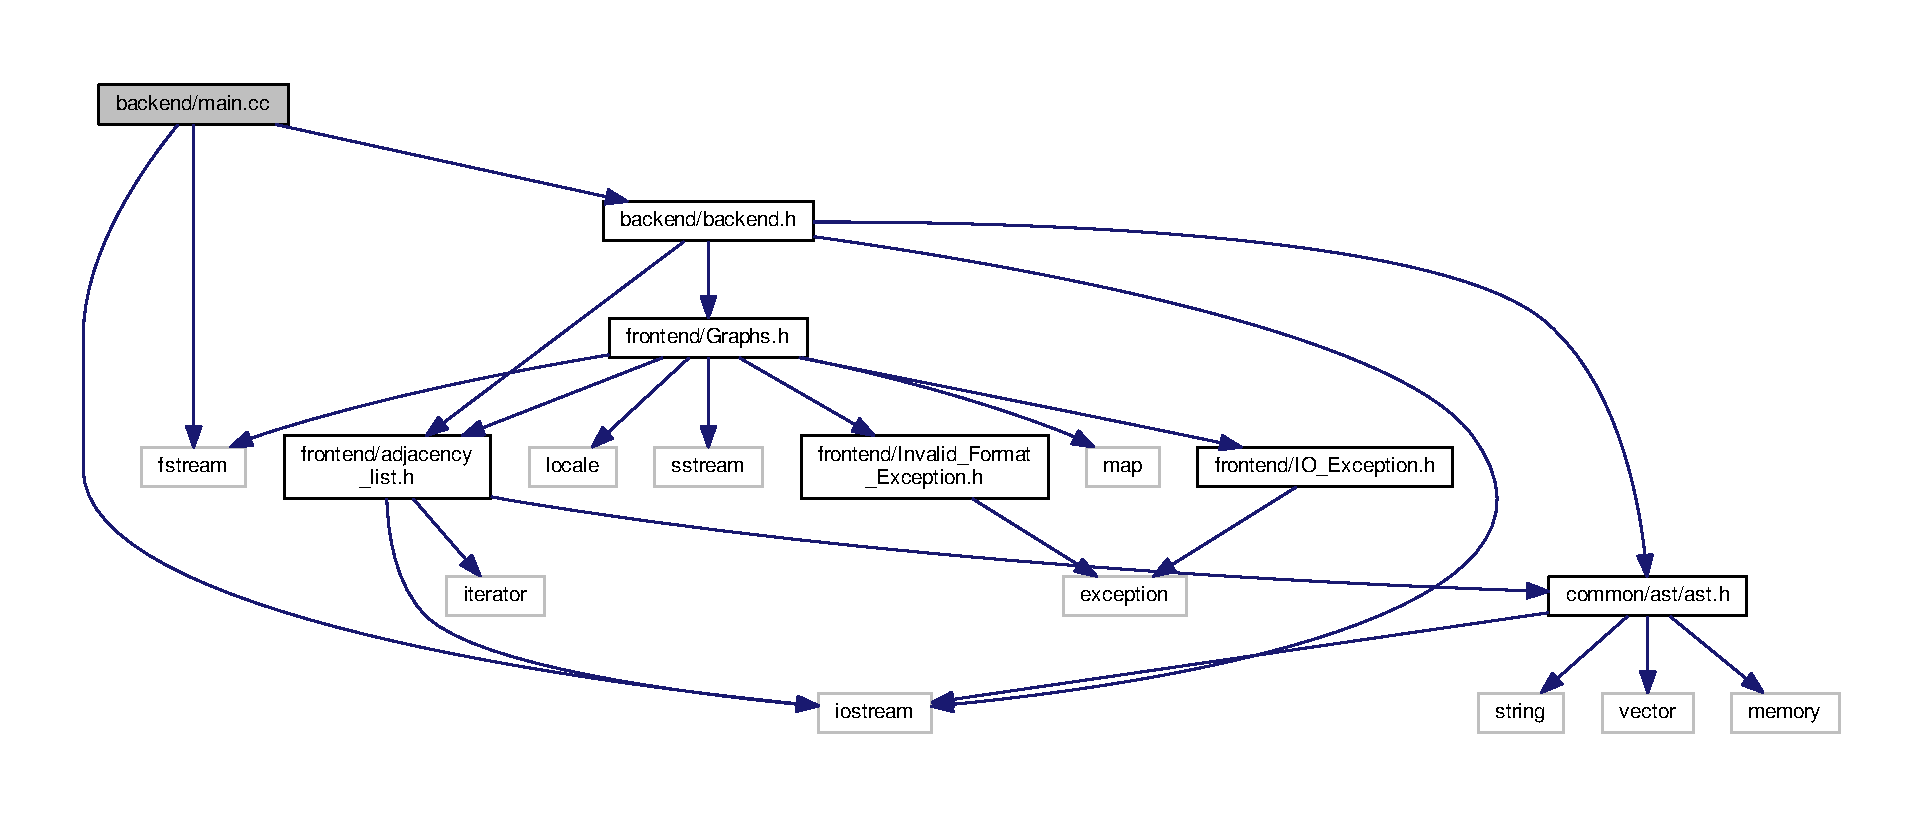
\includegraphics[width=350pt]{main_8cc__incl}
\end{center}
\end{figure}

\hypertarget{ast_8h}{\section{common/ast/ast.h File Reference}
\label{ast_8h}\index{common/ast/ast.\-h@{common/ast/ast.\-h}}
}
{\ttfamily \#include $<$string$>$}\\*
{\ttfamily \#include $<$vector$>$}\\*
{\ttfamily \#include $<$memory$>$}\\*
{\ttfamily \#include $<$iostream$>$}\\*
Include dependency graph for ast.\-h\-:
\nopagebreak
\begin{figure}[H]
\begin{center}
\leavevmode
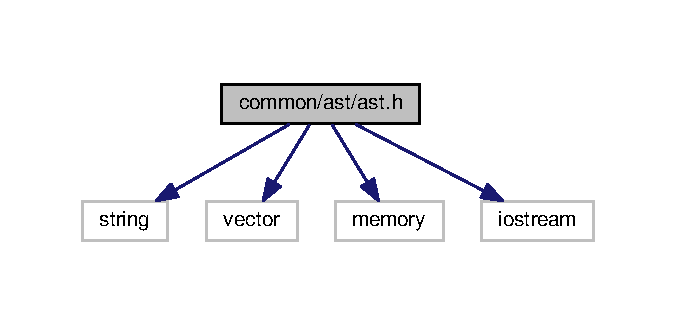
\includegraphics[width=325pt]{ast_8h__incl}
\end{center}
\end{figure}
This graph shows which files directly or indirectly include this file\-:
\nopagebreak
\begin{figure}[H]
\begin{center}
\leavevmode
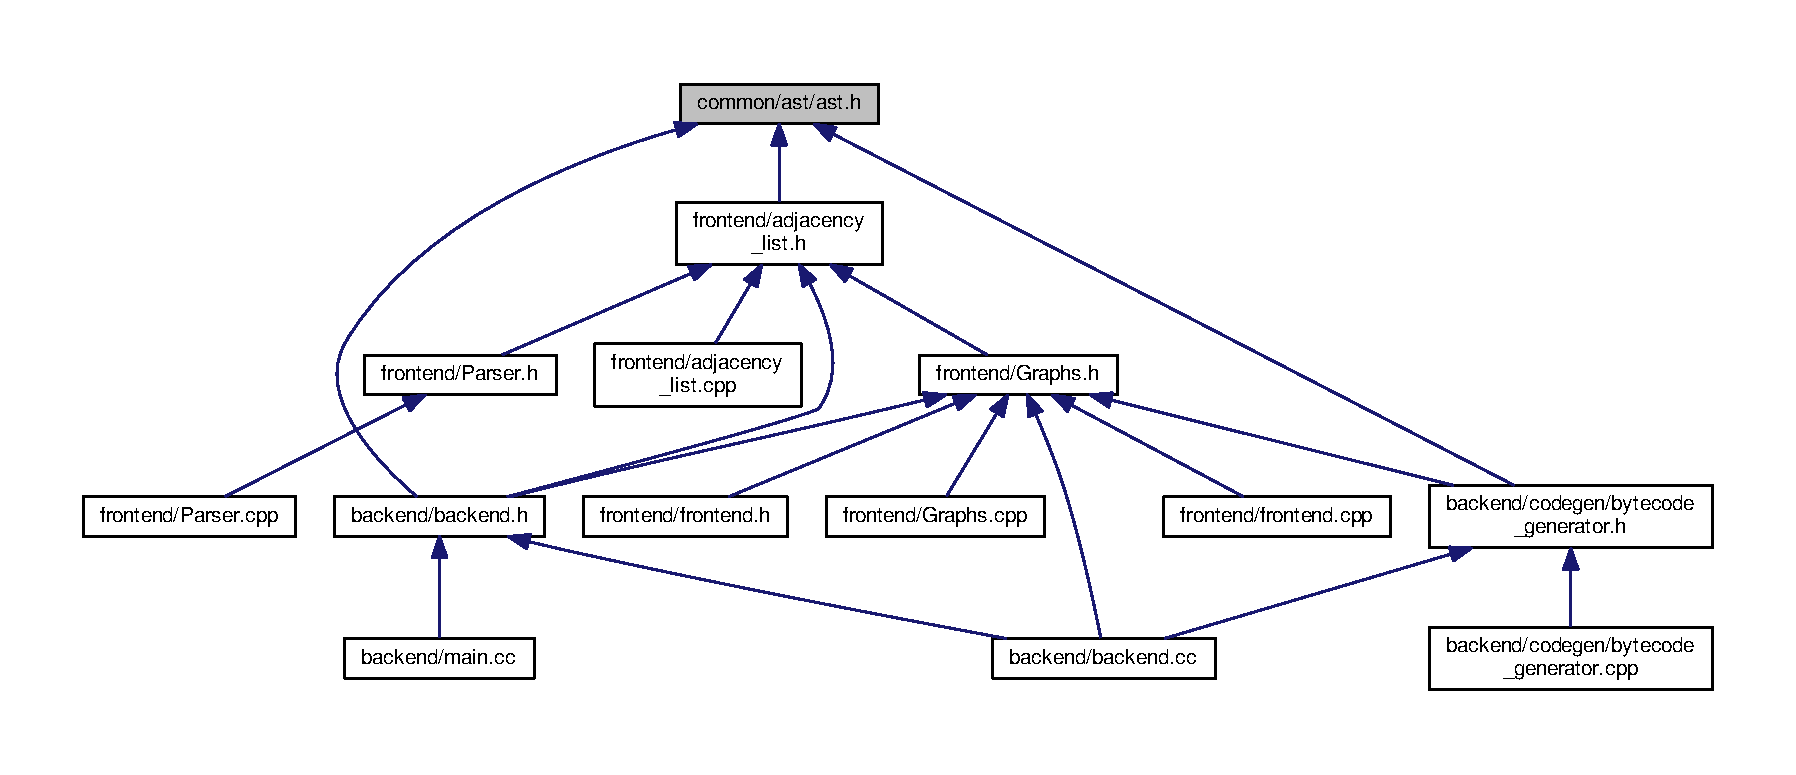
\includegraphics[width=350pt]{ast_8h__dep__incl}
\end{center}
\end{figure}
\subsection*{Classes}
\begin{DoxyCompactItemize}
\item 
struct \hyperlink{structCommand}{Command}
\item 
struct \hyperlink{structNode}{Node}
\item 
class \hyperlink{classGraph}{Graph}
\end{DoxyCompactItemize}

\hypertarget{adjacency__list_8cpp}{\section{frontend/adjacency\-\_\-list.cpp File Reference}
\label{adjacency__list_8cpp}\index{frontend/adjacency\-\_\-list.\-cpp@{frontend/adjacency\-\_\-list.\-cpp}}
}
{\ttfamily \#include $<$frontend/adjacency\-\_\-list.\-h$>$}\\*
Include dependency graph for adjacency\-\_\-list.\-cpp\-:
\nopagebreak
\begin{figure}[H]
\begin{center}
\leavevmode
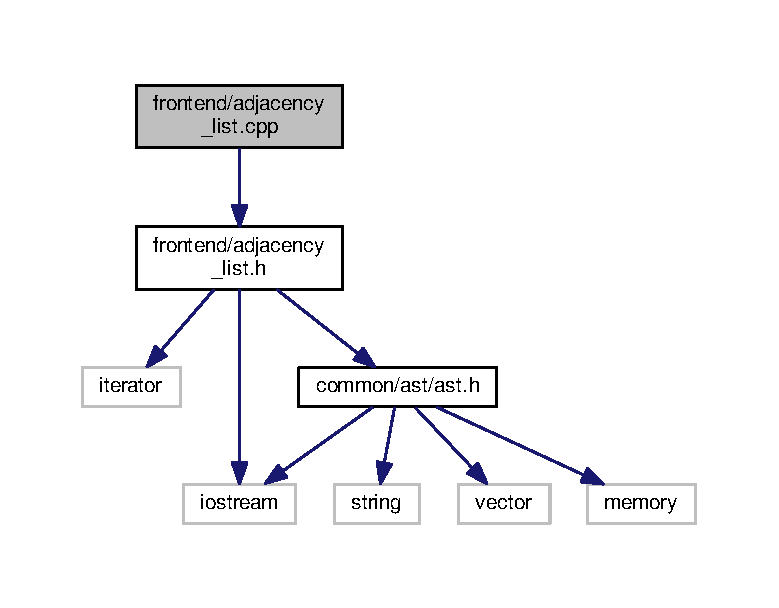
\includegraphics[width=350pt]{adjacency__list_8cpp__incl}
\end{center}
\end{figure}

\hypertarget{adjacency__list_8h}{\section{frontend/adjacency\-\_\-list.h File Reference}
\label{adjacency__list_8h}\index{frontend/adjacency\-\_\-list.\-h@{frontend/adjacency\-\_\-list.\-h}}
}
{\ttfamily \#include $<$iterator$>$}\\*
{\ttfamily \#include $<$iostream$>$}\\*
{\ttfamily \#include $<$common/ast/ast.\-h$>$}\\*
Include dependency graph for adjacency\-\_\-list.\-h\-:
\nopagebreak
\begin{figure}[H]
\begin{center}
\leavevmode
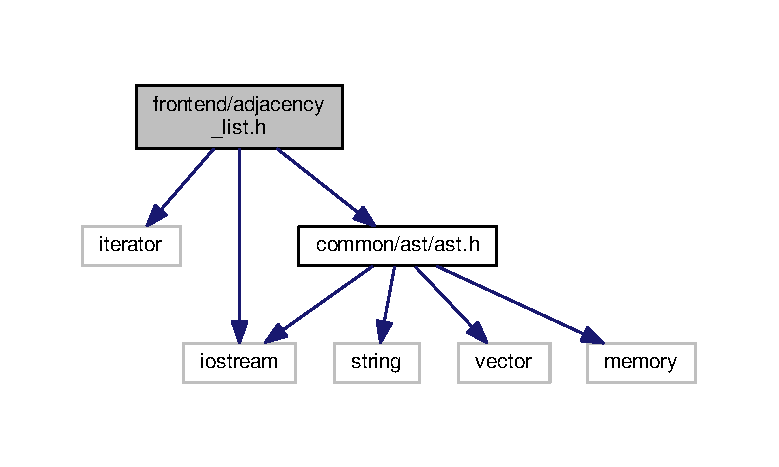
\includegraphics[width=350pt]{adjacency__list_8h__incl}
\end{center}
\end{figure}
This graph shows which files directly or indirectly include this file\-:
\nopagebreak
\begin{figure}[H]
\begin{center}
\leavevmode
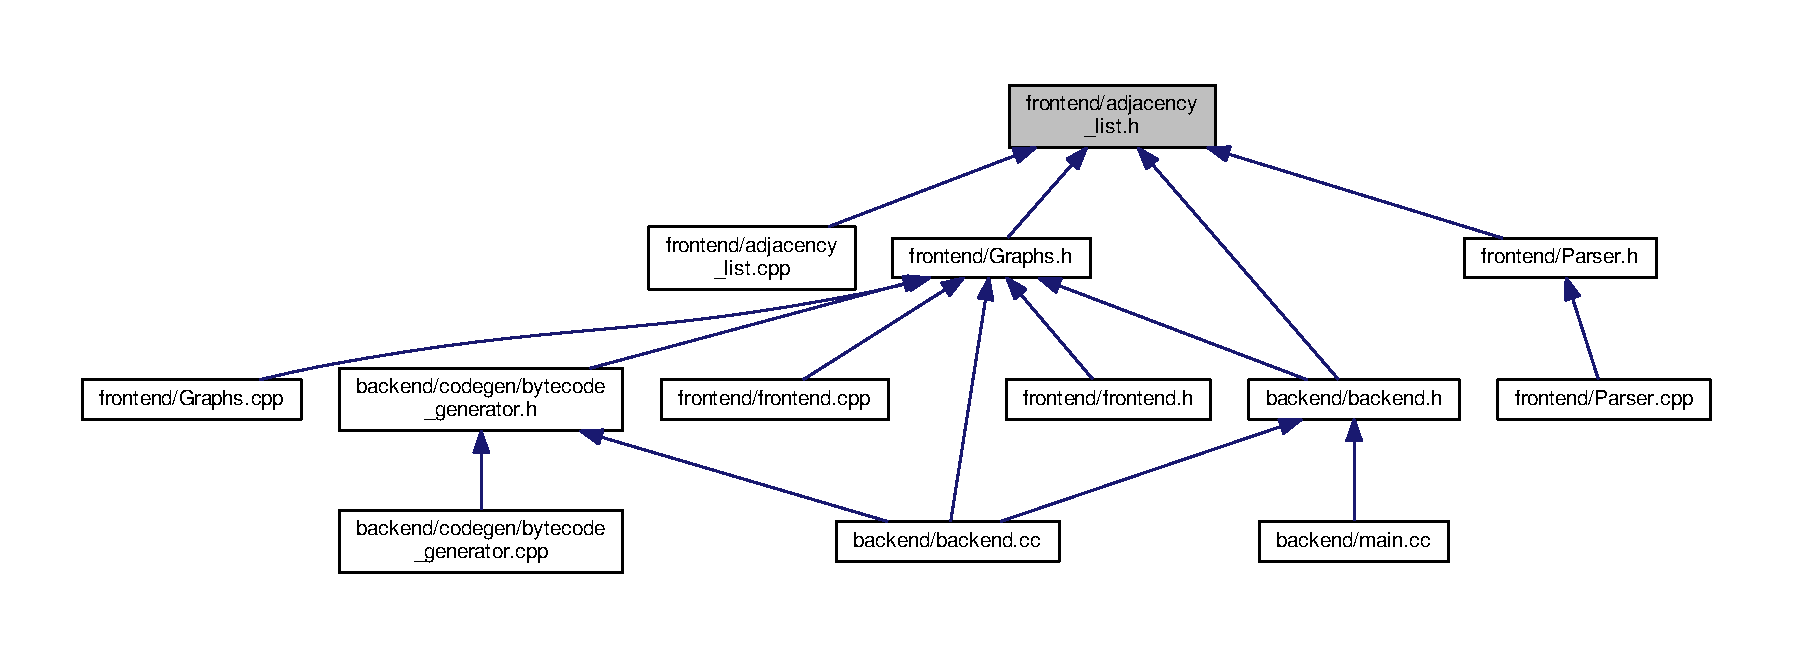
\includegraphics[width=350pt]{adjacency__list_8h__dep__incl}
\end{center}
\end{figure}
\subsection*{Classes}
\begin{DoxyCompactItemize}
\item 
class \hyperlink{classAdjacency__list}{Adjacency\-\_\-list}
\end{DoxyCompactItemize}

\hypertarget{frontend_8cpp}{\section{frontend/frontend.cpp File Reference}
\label{frontend_8cpp}\index{frontend/frontend.\-cpp@{frontend/frontend.\-cpp}}
}
{\ttfamily \#include $<$iostream$>$}\\*
{\ttfamily \#include $<$frontend/\-Graphs.\-h$>$}\\*
Include dependency graph for frontend.\-cpp\-:
\nopagebreak
\begin{figure}[H]
\begin{center}
\leavevmode
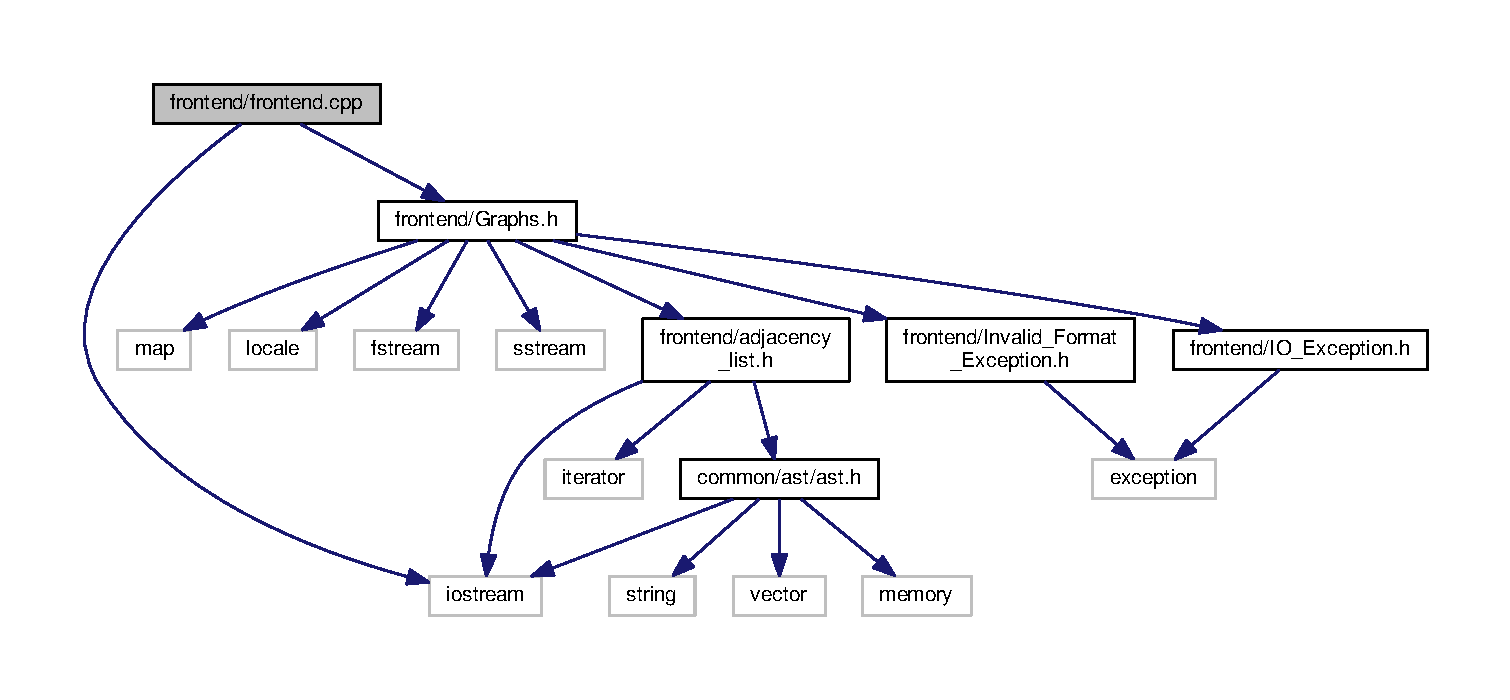
\includegraphics[width=350pt]{frontend_8cpp__incl}
\end{center}
\end{figure}
\subsection*{Functions}
\begin{DoxyCompactItemize}
\item 
int \hyperlink{frontend_8cpp_a51c2e7102bfc166a7268542406dd40f6}{unmarshall\-Graph} (const std\-::string \&file, char delimiter)
\end{DoxyCompactItemize}


\subsection{Function Documentation}
\hypertarget{frontend_8cpp_a51c2e7102bfc166a7268542406dd40f6}{\index{frontend.\-cpp@{frontend.\-cpp}!unmarshall\-Graph@{unmarshall\-Graph}}
\index{unmarshall\-Graph@{unmarshall\-Graph}!frontend.cpp@{frontend.\-cpp}}
\subsubsection[{unmarshall\-Graph}]{\setlength{\rightskip}{0pt plus 5cm}int unmarshall\-Graph (
\begin{DoxyParamCaption}
\item[{const std\-::string \&}]{file, }
\item[{char}]{delimiter}
\end{DoxyParamCaption}
)}}\label{frontend_8cpp_a51c2e7102bfc166a7268542406dd40f6}


Here is the call graph for this function\-:
\nopagebreak
\begin{figure}[H]
\begin{center}
\leavevmode
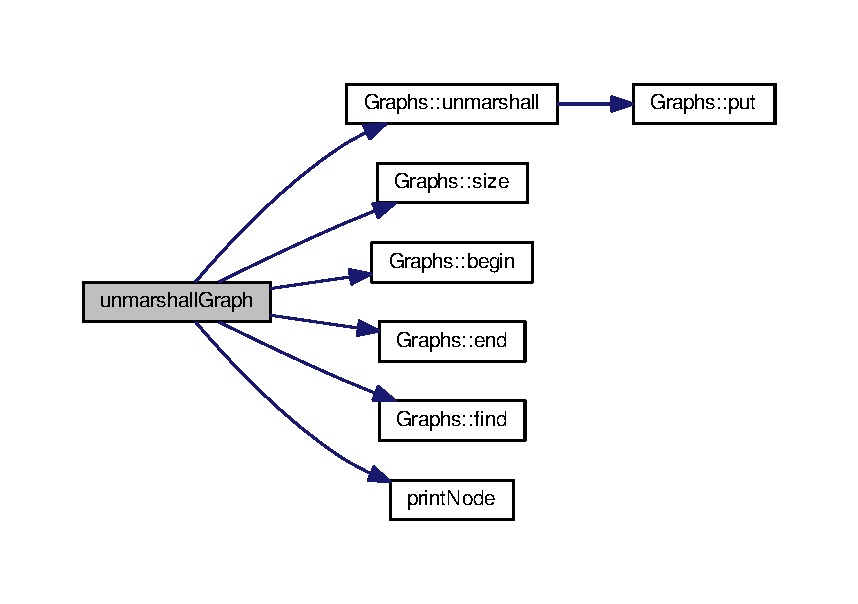
\includegraphics[width=350pt]{frontend_8cpp_a51c2e7102bfc166a7268542406dd40f6_cgraph}
\end{center}
\end{figure}



\hypertarget{frontend_8h}{\section{frontend/frontend.h File Reference}
\label{frontend_8h}\index{frontend/frontend.\-h@{frontend/frontend.\-h}}
}
{\ttfamily \#include $<$iostream$>$}\\*
{\ttfamily \#include $<$frontend/\-Graphs.\-h$>$}\\*
Include dependency graph for frontend.\-h\-:
\nopagebreak
\begin{figure}[H]
\begin{center}
\leavevmode
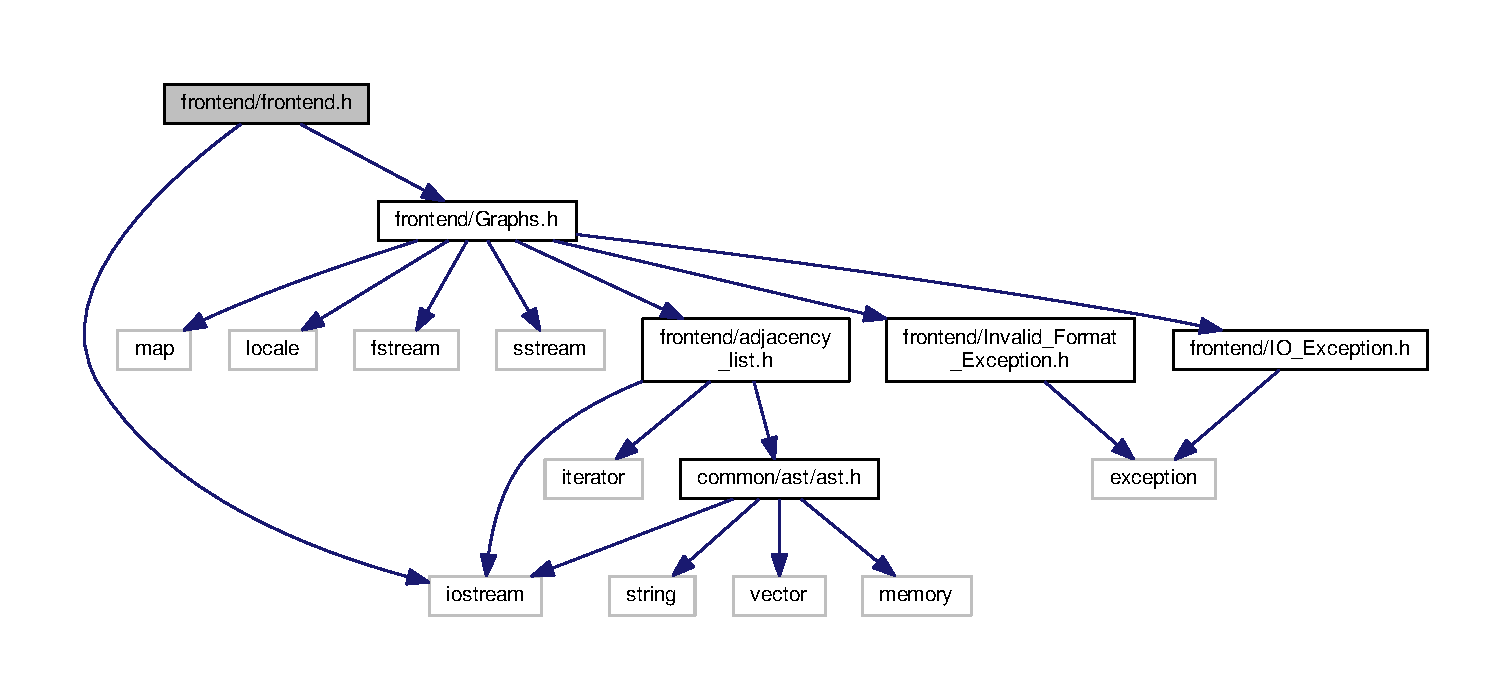
\includegraphics[width=350pt]{frontend_8h__incl}
\end{center}
\end{figure}
\subsection*{Functions}
\begin{DoxyCompactItemize}
\item 
void \hyperlink{frontend_8h_a8e36963ab7eea387d2204a317cb270de}{check\-Vec} (std\-::vector$<$ std\-::string $>$ result)
\item 
int \hyperlink{frontend_8h_a51c2e7102bfc166a7268542406dd40f6}{unmarshall\-Graph} (const std\-::string \&file, char delimiter)
\end{DoxyCompactItemize}


\subsection{Function Documentation}
\hypertarget{frontend_8h_a8e36963ab7eea387d2204a317cb270de}{\index{frontend.\-h@{frontend.\-h}!check\-Vec@{check\-Vec}}
\index{check\-Vec@{check\-Vec}!frontend.h@{frontend.\-h}}
\subsubsection[{check\-Vec}]{\setlength{\rightskip}{0pt plus 5cm}void check\-Vec (
\begin{DoxyParamCaption}
\item[{std\-::vector$<$ std\-::string $>$}]{result}
\end{DoxyParamCaption}
)}}\label{frontend_8h_a8e36963ab7eea387d2204a317cb270de}
\hypertarget{frontend_8h_a51c2e7102bfc166a7268542406dd40f6}{\index{frontend.\-h@{frontend.\-h}!unmarshall\-Graph@{unmarshall\-Graph}}
\index{unmarshall\-Graph@{unmarshall\-Graph}!frontend.h@{frontend.\-h}}
\subsubsection[{unmarshall\-Graph}]{\setlength{\rightskip}{0pt plus 5cm}int unmarshall\-Graph (
\begin{DoxyParamCaption}
\item[{const std\-::string \&}]{file, }
\item[{char}]{delimiter}
\end{DoxyParamCaption}
)}}\label{frontend_8h_a51c2e7102bfc166a7268542406dd40f6}


Here is the call graph for this function\-:
\nopagebreak
\begin{figure}[H]
\begin{center}
\leavevmode
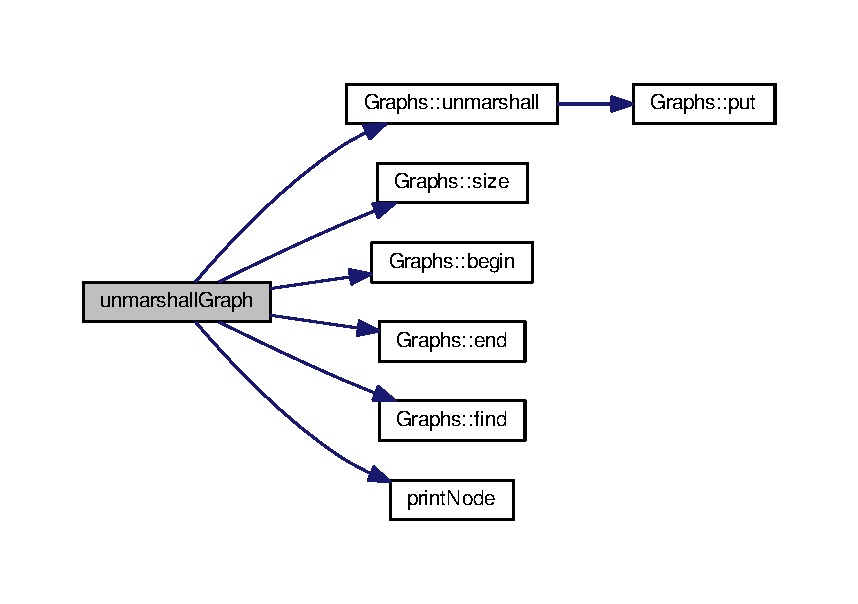
\includegraphics[width=350pt]{frontend_8h_a51c2e7102bfc166a7268542406dd40f6_cgraph}
\end{center}
\end{figure}



\hypertarget{Graphs_8cpp}{\section{frontend/\-Graphs.cpp File Reference}
\label{Graphs_8cpp}\index{frontend/\-Graphs.\-cpp@{frontend/\-Graphs.\-cpp}}
}
{\ttfamily \#include $<$frontend/\-Graphs.\-h$>$}\\*
Include dependency graph for Graphs.\-cpp\-:
\nopagebreak
\begin{figure}[H]
\begin{center}
\leavevmode
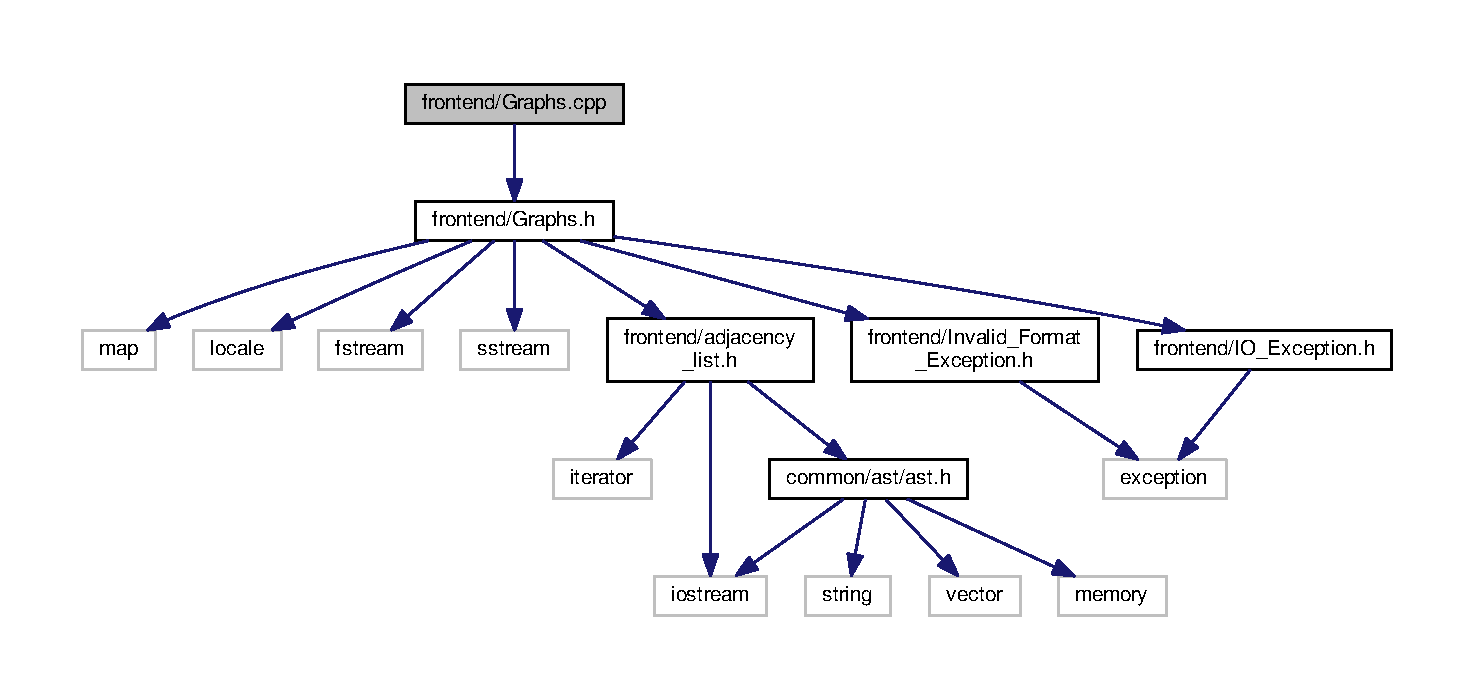
\includegraphics[width=350pt]{Graphs_8cpp__incl}
\end{center}
\end{figure}
\subsection*{Functions}
\begin{DoxyCompactItemize}
\item 
void \hyperlink{Graphs_8cpp_a3c083ba3ce77f57bb61674b3792475d5}{print\-Node} (std\-::shared\-\_\-ptr$<$ \hyperlink{structNode}{Node} $>$ n)
\end{DoxyCompactItemize}


\subsection{Function Documentation}
\hypertarget{Graphs_8cpp_a3c083ba3ce77f57bb61674b3792475d5}{\index{Graphs.\-cpp@{Graphs.\-cpp}!print\-Node@{print\-Node}}
\index{print\-Node@{print\-Node}!Graphs.cpp@{Graphs.\-cpp}}
\subsubsection[{print\-Node}]{\setlength{\rightskip}{0pt plus 5cm}void print\-Node (
\begin{DoxyParamCaption}
\item[{std\-::shared\-\_\-ptr$<$ {\bf Node} $>$}]{n}
\end{DoxyParamCaption}
)}}\label{Graphs_8cpp_a3c083ba3ce77f57bb61674b3792475d5}

\hypertarget{Graphs_8h}{\section{frontend/\-Graphs.h File Reference}
\label{Graphs_8h}\index{frontend/\-Graphs.\-h@{frontend/\-Graphs.\-h}}
}
{\ttfamily \#include $<$map$>$}\\*
{\ttfamily \#include $<$locale$>$}\\*
{\ttfamily \#include $<$fstream$>$}\\*
{\ttfamily \#include $<$sstream$>$}\\*
{\ttfamily \#include $<$frontend/adjacency\-\_\-list.\-h$>$}\\*
{\ttfamily \#include $<$frontend/\-Invalid\-\_\-\-Format\-\_\-\-Exception.\-h$>$}\\*
{\ttfamily \#include $<$frontend/\-I\-O\-\_\-\-Exception.\-h$>$}\\*
Include dependency graph for Graphs.\-h\-:
\nopagebreak
\begin{figure}[H]
\begin{center}
\leavevmode
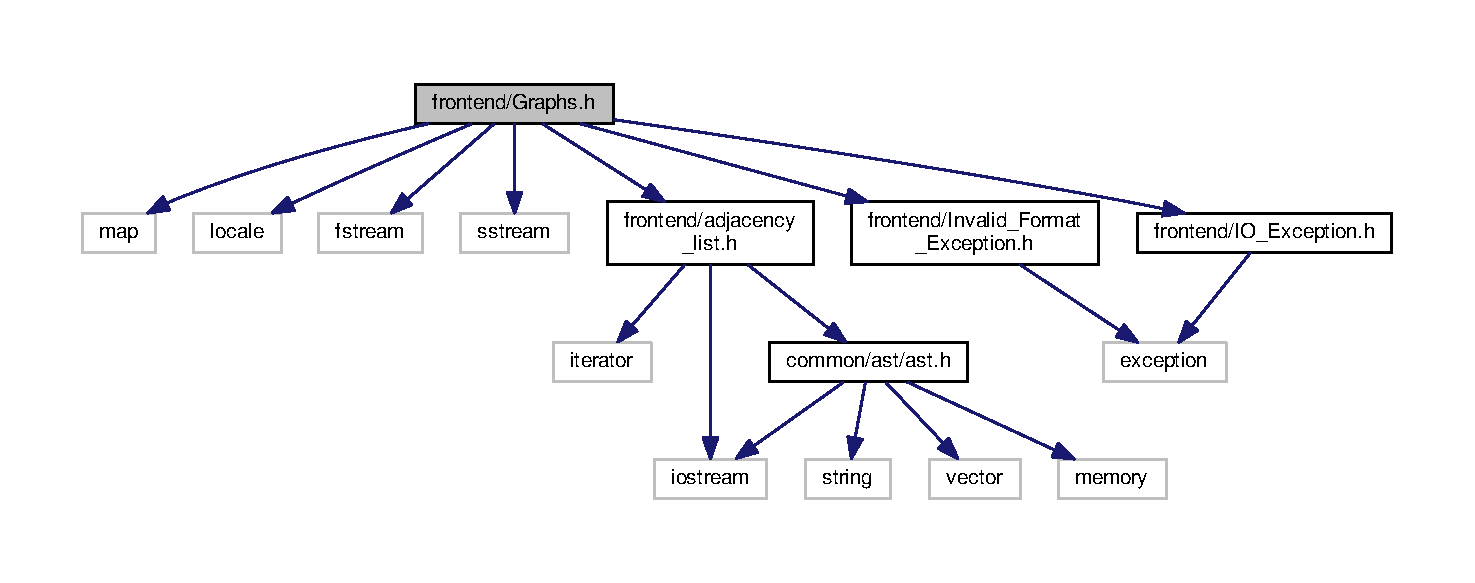
\includegraphics[width=350pt]{Graphs_8h__incl}
\end{center}
\end{figure}
This graph shows which files directly or indirectly include this file\-:
\nopagebreak
\begin{figure}[H]
\begin{center}
\leavevmode
\includegraphics[width=350pt]{Graphs_8h__dep__incl}
\end{center}
\end{figure}
\subsection*{Classes}
\begin{DoxyCompactItemize}
\item 
class \hyperlink{classGraphs}{Graphs}
\end{DoxyCompactItemize}
\subsection*{Functions}
\begin{DoxyCompactItemize}
\item 
void \hyperlink{Graphs_8h_a0e3ec1a2bedc6726cf02cd1c981bb2ea}{print\-Node} (\hyperlink{classGraphs_a2804b752d72989344f11a6ec3145eea8}{Graphs\-::\-Node\-\_\-ptr} n)
\end{DoxyCompactItemize}


\subsection{Function Documentation}
\hypertarget{Graphs_8h_a0e3ec1a2bedc6726cf02cd1c981bb2ea}{\index{Graphs.\-h@{Graphs.\-h}!print\-Node@{print\-Node}}
\index{print\-Node@{print\-Node}!Graphs.h@{Graphs.\-h}}
\subsubsection[{print\-Node}]{\setlength{\rightskip}{0pt plus 5cm}void print\-Node (
\begin{DoxyParamCaption}
\item[{{\bf Graphs\-::\-Node\-\_\-ptr}}]{n}
\end{DoxyParamCaption}
)}}\label{Graphs_8h_a0e3ec1a2bedc6726cf02cd1c981bb2ea}

\hypertarget{Invalid__Format__Exception_8h}{\section{frontend/\-Invalid\-\_\-\-Format\-\_\-\-Exception.h File Reference}
\label{Invalid__Format__Exception_8h}\index{frontend/\-Invalid\-\_\-\-Format\-\_\-\-Exception.\-h@{frontend/\-Invalid\-\_\-\-Format\-\_\-\-Exception.\-h}}
}
{\ttfamily \#include $<$exception$>$}\\*
Include dependency graph for Invalid\-\_\-\-Format\-\_\-\-Exception.\-h\-:
\nopagebreak
\begin{figure}[H]
\begin{center}
\leavevmode
\includegraphics[width=198pt]{Invalid__Format__Exception_8h__incl}
\end{center}
\end{figure}
This graph shows which files directly or indirectly include this file\-:
\nopagebreak
\begin{figure}[H]
\begin{center}
\leavevmode
\includegraphics[width=350pt]{Invalid__Format__Exception_8h__dep__incl}
\end{center}
\end{figure}
\subsection*{Classes}
\begin{DoxyCompactItemize}
\item 
class \hyperlink{classInvalid__Format__Exception}{Invalid\-\_\-\-Format\-\_\-\-Exception}
\end{DoxyCompactItemize}

\hypertarget{IO__Exception_8h}{\section{frontend/\-I\-O\-\_\-\-Exception.h File Reference}
\label{IO__Exception_8h}\index{frontend/\-I\-O\-\_\-\-Exception.\-h@{frontend/\-I\-O\-\_\-\-Exception.\-h}}
}
{\ttfamily \#include $<$exception$>$}\\*
Include dependency graph for I\-O\-\_\-\-Exception.\-h\-:
\nopagebreak
\begin{figure}[H]
\begin{center}
\leavevmode
\includegraphics[width=202pt]{IO__Exception_8h__incl}
\end{center}
\end{figure}
This graph shows which files directly or indirectly include this file\-:
\nopagebreak
\begin{figure}[H]
\begin{center}
\leavevmode
\includegraphics[width=350pt]{IO__Exception_8h__dep__incl}
\end{center}
\end{figure}
\subsection*{Classes}
\begin{DoxyCompactItemize}
\item 
class \hyperlink{classIO__Exception}{I\-O\-\_\-\-Exception}
\end{DoxyCompactItemize}

\hypertarget{lexer_8cpp}{\section{frontend/parse/lexer.cpp File Reference}
\label{lexer_8cpp}\index{frontend/parse/lexer.\-cpp@{frontend/parse/lexer.\-cpp}}
}
{\ttfamily \#include $<$frontend/parse/lexer.\-h$>$}\\*
Include dependency graph for lexer.\-cpp\-:
\nopagebreak
\begin{figure}[H]
\begin{center}
\leavevmode
\includegraphics[width=350pt]{lexer_8cpp__incl}
\end{center}
\end{figure}

\hypertarget{lexer_8h}{\section{frontend/parse/lexer.h File Reference}
\label{lexer_8h}\index{frontend/parse/lexer.\-h@{frontend/parse/lexer.\-h}}
}
{\ttfamily \#include $<$iostream$>$}\\*
{\ttfamily \#include $<$fstream$>$}\\*
{\ttfamily \#include $<$cstring$>$}\\*
{\ttfamily \#include $<$vector$>$}\\*
{\ttfamily \#include $<$frontend/\-I\-O\-\_\-\-Exception.\-h$>$}\\*
Include dependency graph for lexer.\-h\-:
\nopagebreak
\begin{figure}[H]
\begin{center}
\leavevmode
\includegraphics[width=350pt]{lexer_8h__incl}
\end{center}
\end{figure}
This graph shows which files directly or indirectly include this file\-:
\nopagebreak
\begin{figure}[H]
\begin{center}
\leavevmode
\includegraphics[width=202pt]{lexer_8h__dep__incl}
\end{center}
\end{figure}
\subsection*{Classes}
\begin{DoxyCompactItemize}
\item 
class \hyperlink{classRailFunction}{Rail\-Function}
\item 
class \hyperlink{classLexer}{Lexer}
\end{DoxyCompactItemize}
\subsection*{Variables}
\begin{DoxyCompactItemize}
\item 
const int \hyperlink{lexer_8h_a3b95e0254661c995b723a9b150a821c1}{M\-A\-X\-\_\-\-C\-H\-A\-R\-S\-\_\-\-P\-E\-R\-\_\-\-L\-I\-N\-E} = 1024
\item 
const int \hyperlink{lexer_8h_afe8deb2b6b8318fa96d532e836f97a20}{M\-A\-X\-\_\-\-L\-I\-N\-E\-S\-\_\-\-P\-E\-R\-\_\-\-F\-U\-N\-C\-T\-I\-O\-N} = 1024
\end{DoxyCompactItemize}


\subsection{Variable Documentation}
\hypertarget{lexer_8h_a3b95e0254661c995b723a9b150a821c1}{\index{lexer.\-h@{lexer.\-h}!M\-A\-X\-\_\-\-C\-H\-A\-R\-S\-\_\-\-P\-E\-R\-\_\-\-L\-I\-N\-E@{M\-A\-X\-\_\-\-C\-H\-A\-R\-S\-\_\-\-P\-E\-R\-\_\-\-L\-I\-N\-E}}
\index{M\-A\-X\-\_\-\-C\-H\-A\-R\-S\-\_\-\-P\-E\-R\-\_\-\-L\-I\-N\-E@{M\-A\-X\-\_\-\-C\-H\-A\-R\-S\-\_\-\-P\-E\-R\-\_\-\-L\-I\-N\-E}!lexer.h@{lexer.\-h}}
\subsubsection[{M\-A\-X\-\_\-\-C\-H\-A\-R\-S\-\_\-\-P\-E\-R\-\_\-\-L\-I\-N\-E}]{\setlength{\rightskip}{0pt plus 5cm}const int M\-A\-X\-\_\-\-C\-H\-A\-R\-S\-\_\-\-P\-E\-R\-\_\-\-L\-I\-N\-E = 1024}}\label{lexer_8h_a3b95e0254661c995b723a9b150a821c1}
\hypertarget{lexer_8h_afe8deb2b6b8318fa96d532e836f97a20}{\index{lexer.\-h@{lexer.\-h}!M\-A\-X\-\_\-\-L\-I\-N\-E\-S\-\_\-\-P\-E\-R\-\_\-\-F\-U\-N\-C\-T\-I\-O\-N@{M\-A\-X\-\_\-\-L\-I\-N\-E\-S\-\_\-\-P\-E\-R\-\_\-\-F\-U\-N\-C\-T\-I\-O\-N}}
\index{M\-A\-X\-\_\-\-L\-I\-N\-E\-S\-\_\-\-P\-E\-R\-\_\-\-F\-U\-N\-C\-T\-I\-O\-N@{M\-A\-X\-\_\-\-L\-I\-N\-E\-S\-\_\-\-P\-E\-R\-\_\-\-F\-U\-N\-C\-T\-I\-O\-N}!lexer.h@{lexer.\-h}}
\subsubsection[{M\-A\-X\-\_\-\-L\-I\-N\-E\-S\-\_\-\-P\-E\-R\-\_\-\-F\-U\-N\-C\-T\-I\-O\-N}]{\setlength{\rightskip}{0pt plus 5cm}const int M\-A\-X\-\_\-\-L\-I\-N\-E\-S\-\_\-\-P\-E\-R\-\_\-\-F\-U\-N\-C\-T\-I\-O\-N = 1024}}\label{lexer_8h_afe8deb2b6b8318fa96d532e836f97a20}

\hypertarget{zustaende_8md}{\section{frontend/parse/zustaende.md File Reference}
\label{zustaende_8md}\index{frontend/parse/zustaende.\-md@{frontend/parse/zustaende.\-md}}
}

\hypertarget{Parse__Exception_8h}{\section{frontend/\-Parse\-\_\-\-Exception.h File Reference}
\label{Parse__Exception_8h}\index{frontend/\-Parse\-\_\-\-Exception.\-h@{frontend/\-Parse\-\_\-\-Exception.\-h}}
}
{\ttfamily \#include $<$exception$>$}\\*
{\ttfamily \#include $<$sstream$>$}\\*
Include dependency graph for Parse\-\_\-\-Exception.\-h\-:
\nopagebreak
\begin{figure}[H]
\begin{center}
\leavevmode
\includegraphics[width=216pt]{Parse__Exception_8h__incl}
\end{center}
\end{figure}
\subsection*{Classes}
\begin{DoxyCompactItemize}
\item 
class \hyperlink{classParse__Exception}{Parse\-\_\-\-Exception}
\end{DoxyCompactItemize}

\hypertarget{Parser_8cpp}{\section{frontend/\-Parser.cpp File Reference}
\label{Parser_8cpp}\index{frontend/\-Parser.\-cpp@{frontend/\-Parser.\-cpp}}
}
{\ttfamily \#include $<$frontend/\-Parser.\-h$>$}\\*
Include dependency graph for Parser.\-cpp\-:
\nopagebreak
\begin{figure}[H]
\begin{center}
\leavevmode
\includegraphics[width=350pt]{Parser_8cpp__incl}
\end{center}
\end{figure}
\subsection*{Functions}
\begin{DoxyCompactItemize}
\item 
std\-::list$<$ char $>$ \hyperlink{Parser_8cpp_aab424582145aad704b43acc661ab744f}{list\-From\-Array} (char chars\mbox{[}$\,$\mbox{]}, int size)
\end{DoxyCompactItemize}


\subsection{Function Documentation}
\hypertarget{Parser_8cpp_aab424582145aad704b43acc661ab744f}{\index{Parser.\-cpp@{Parser.\-cpp}!list\-From\-Array@{list\-From\-Array}}
\index{list\-From\-Array@{list\-From\-Array}!Parser.cpp@{Parser.\-cpp}}
\subsubsection[{list\-From\-Array}]{\setlength{\rightskip}{0pt plus 5cm}std\-::list$<$char$>$ list\-From\-Array (
\begin{DoxyParamCaption}
\item[{char}]{chars\mbox{[}$\,$\mbox{]}, }
\item[{int}]{size}
\end{DoxyParamCaption}
)}}\label{Parser_8cpp_aab424582145aad704b43acc661ab744f}

\hypertarget{Parser_8h}{\section{frontend/\-Parser.h File Reference}
\label{Parser_8h}\index{frontend/\-Parser.\-h@{frontend/\-Parser.\-h}}
}
{\ttfamily \#include $<$list$>$}\\*
{\ttfamily \#include $<$map$>$}\\*
{\ttfamily \#include $<$string$>$}\\*
{\ttfamily \#include $<$algorithm$>$}\\*
{\ttfamily \#include $<$iostream$>$}\\*
{\ttfamily \#include $<$sstream$>$}\\*
{\ttfamily \#include $<$frontend/adjacency\-\_\-list.\-h$>$}\\*
Include dependency graph for Parser.\-h\-:
\nopagebreak
\begin{figure}[H]
\begin{center}
\leavevmode
\includegraphics[width=350pt]{Parser_8h__incl}
\end{center}
\end{figure}
This graph shows which files directly or indirectly include this file\-:
\nopagebreak
\begin{figure}[H]
\begin{center}
\leavevmode
\includegraphics[width=180pt]{Parser_8h__dep__incl}
\end{center}
\end{figure}
\subsection*{Classes}
\begin{DoxyCompactItemize}
\item 
struct \hyperlink{structoffsetvalues}{offsetvalues}
\item 
struct \hyperlink{structallowedChars}{allowed\-Chars}
\item 
struct \hyperlink{structBoardContainer}{Board\-Container}
\item 
class \hyperlink{classParser}{Parser}
\end{DoxyCompactItemize}
\subsection*{Enumerations}
\begin{DoxyCompactItemize}
\item 
enum \hyperlink{Parser_8h_a224b9163917ac32fc95a60d8c1eec3aa}{Direction} \{ \\*
\hyperlink{Parser_8h_a224b9163917ac32fc95a60d8c1eec3aaab199e021998d49b1f09338d8b9b18ecb}{E} =0, 
\hyperlink{Parser_8h_a224b9163917ac32fc95a60d8c1eec3aaa61c600c17d14bd4db73433ddbb8491e8}{S\-E} =1, 
\hyperlink{Parser_8h_a224b9163917ac32fc95a60d8c1eec3aaaf1ce01387d2348f8b858721a7db81670}{S} =2, 
\hyperlink{Parser_8h_a224b9163917ac32fc95a60d8c1eec3aaa247b880fc48dc1c74961ba58ae0f68a2}{S\-W} =3, 
\\*
\hyperlink{Parser_8h_a224b9163917ac32fc95a60d8c1eec3aaab722ceeb601c72cd78fbd35f3581fdf7}{W} =4, 
\hyperlink{Parser_8h_a224b9163917ac32fc95a60d8c1eec3aaa9b2eeb9b33247edbc638099452c6b46f}{N\-W} =5, 
\hyperlink{Parser_8h_a224b9163917ac32fc95a60d8c1eec3aaa2c63acbe79d9f41ba6bb7766e9c37702}{N} =6, 
\hyperlink{Parser_8h_a224b9163917ac32fc95a60d8c1eec3aaa4d3f872f5054b256b01ee4f2c8cf51db}{N\-E} =7
 \}
\end{DoxyCompactItemize}


\subsection{Enumeration Type Documentation}
\hypertarget{Parser_8h_a224b9163917ac32fc95a60d8c1eec3aa}{\index{Parser.\-h@{Parser.\-h}!Direction@{Direction}}
\index{Direction@{Direction}!Parser.h@{Parser.\-h}}
\subsubsection[{Direction}]{\setlength{\rightskip}{0pt plus 5cm}enum {\bf Direction}}}\label{Parser_8h_a224b9163917ac32fc95a60d8c1eec3aa}
\begin{Desc}
\item[Enumerator]\par
\begin{description}
\index{E@{E}!Parser.\-h@{Parser.\-h}}\index{Parser.\-h@{Parser.\-h}!E@{E}}\item[{\em 
\hypertarget{Parser_8h_a224b9163917ac32fc95a60d8c1eec3aaab199e021998d49b1f09338d8b9b18ecb}{E}\label{Parser_8h_a224b9163917ac32fc95a60d8c1eec3aaab199e021998d49b1f09338d8b9b18ecb}
}]\index{S\-E@{S\-E}!Parser.\-h@{Parser.\-h}}\index{Parser.\-h@{Parser.\-h}!S\-E@{S\-E}}\item[{\em 
\hypertarget{Parser_8h_a224b9163917ac32fc95a60d8c1eec3aaa61c600c17d14bd4db73433ddbb8491e8}{S\-E}\label{Parser_8h_a224b9163917ac32fc95a60d8c1eec3aaa61c600c17d14bd4db73433ddbb8491e8}
}]\index{S@{S}!Parser.\-h@{Parser.\-h}}\index{Parser.\-h@{Parser.\-h}!S@{S}}\item[{\em 
\hypertarget{Parser_8h_a224b9163917ac32fc95a60d8c1eec3aaaf1ce01387d2348f8b858721a7db81670}{S}\label{Parser_8h_a224b9163917ac32fc95a60d8c1eec3aaaf1ce01387d2348f8b858721a7db81670}
}]\index{S\-W@{S\-W}!Parser.\-h@{Parser.\-h}}\index{Parser.\-h@{Parser.\-h}!S\-W@{S\-W}}\item[{\em 
\hypertarget{Parser_8h_a224b9163917ac32fc95a60d8c1eec3aaa247b880fc48dc1c74961ba58ae0f68a2}{S\-W}\label{Parser_8h_a224b9163917ac32fc95a60d8c1eec3aaa247b880fc48dc1c74961ba58ae0f68a2}
}]\index{W@{W}!Parser.\-h@{Parser.\-h}}\index{Parser.\-h@{Parser.\-h}!W@{W}}\item[{\em 
\hypertarget{Parser_8h_a224b9163917ac32fc95a60d8c1eec3aaab722ceeb601c72cd78fbd35f3581fdf7}{W}\label{Parser_8h_a224b9163917ac32fc95a60d8c1eec3aaab722ceeb601c72cd78fbd35f3581fdf7}
}]\index{N\-W@{N\-W}!Parser.\-h@{Parser.\-h}}\index{Parser.\-h@{Parser.\-h}!N\-W@{N\-W}}\item[{\em 
\hypertarget{Parser_8h_a224b9163917ac32fc95a60d8c1eec3aaa9b2eeb9b33247edbc638099452c6b46f}{N\-W}\label{Parser_8h_a224b9163917ac32fc95a60d8c1eec3aaa9b2eeb9b33247edbc638099452c6b46f}
}]\index{N@{N}!Parser.\-h@{Parser.\-h}}\index{Parser.\-h@{Parser.\-h}!N@{N}}\item[{\em 
\hypertarget{Parser_8h_a224b9163917ac32fc95a60d8c1eec3aaa2c63acbe79d9f41ba6bb7766e9c37702}{N}\label{Parser_8h_a224b9163917ac32fc95a60d8c1eec3aaa2c63acbe79d9f41ba6bb7766e9c37702}
}]\index{N\-E@{N\-E}!Parser.\-h@{Parser.\-h}}\index{Parser.\-h@{Parser.\-h}!N\-E@{N\-E}}\item[{\em 
\hypertarget{Parser_8h_a224b9163917ac32fc95a60d8c1eec3aaa4d3f872f5054b256b01ee4f2c8cf51db}{N\-E}\label{Parser_8h_a224b9163917ac32fc95a60d8c1eec3aaa4d3f872f5054b256b01ee4f2c8cf51db}
}]\end{description}
\end{Desc}

%--- End generated contents ---

% Index
\newpage
\phantomsection
\addcontentsline{toc}{chapter}{Index}
\printindex

\end{document}
